% Options for packages loaded elsewhere
\PassOptionsToPackage{unicode}{hyperref}
\PassOptionsToPackage{hyphens}{url}
\PassOptionsToPackage{dvipsnames,svgnames,x11names}{xcolor}
%
\documentclass[
  a4paper,
  DIV=11,
  numbers=noendperiod]{scrartcl}

\usepackage{amsmath,amssymb}
\usepackage{iftex}
\ifPDFTeX
  \usepackage[T1]{fontenc}
  \usepackage[utf8]{inputenc}
  \usepackage{textcomp} % provide euro and other symbols
\else % if luatex or xetex
  \usepackage{unicode-math}
  \defaultfontfeatures{Scale=MatchLowercase}
  \defaultfontfeatures[\rmfamily]{Ligatures=TeX,Scale=1}
\fi
\usepackage{lmodern}
\ifPDFTeX\else  
    % xetex/luatex font selection
\fi
% Use upquote if available, for straight quotes in verbatim environments
\IfFileExists{upquote.sty}{\usepackage{upquote}}{}
\IfFileExists{microtype.sty}{% use microtype if available
  \usepackage[]{microtype}
  \UseMicrotypeSet[protrusion]{basicmath} % disable protrusion for tt fonts
}{}
\makeatletter
\@ifundefined{KOMAClassName}{% if non-KOMA class
  \IfFileExists{parskip.sty}{%
    \usepackage{parskip}
  }{% else
    \setlength{\parindent}{0pt}
    \setlength{\parskip}{6pt plus 2pt minus 1pt}}
}{% if KOMA class
  \KOMAoptions{parskip=half}}
\makeatother
\usepackage{xcolor}
\setlength{\emergencystretch}{3em} % prevent overfull lines
\setcounter{secnumdepth}{-\maxdimen} % remove section numbering
% Make \paragraph and \subparagraph free-standing
\makeatletter
\ifx\paragraph\undefined\else
  \let\oldparagraph\paragraph
  \renewcommand{\paragraph}{
    \@ifstar
      \xxxParagraphStar
      \xxxParagraphNoStar
  }
  \newcommand{\xxxParagraphStar}[1]{\oldparagraph*{#1}\mbox{}}
  \newcommand{\xxxParagraphNoStar}[1]{\oldparagraph{#1}\mbox{}}
\fi
\ifx\subparagraph\undefined\else
  \let\oldsubparagraph\subparagraph
  \renewcommand{\subparagraph}{
    \@ifstar
      \xxxSubParagraphStar
      \xxxSubParagraphNoStar
  }
  \newcommand{\xxxSubParagraphStar}[1]{\oldsubparagraph*{#1}\mbox{}}
  \newcommand{\xxxSubParagraphNoStar}[1]{\oldsubparagraph{#1}\mbox{}}
\fi
\makeatother

\usepackage{color}
\usepackage{fancyvrb}
\newcommand{\VerbBar}{|}
\newcommand{\VERB}{\Verb[commandchars=\\\{\}]}
\DefineVerbatimEnvironment{Highlighting}{Verbatim}{commandchars=\\\{\}}
% Add ',fontsize=\small' for more characters per line
\usepackage{framed}
\definecolor{shadecolor}{RGB}{241,243,245}
\newenvironment{Shaded}{\begin{snugshade}}{\end{snugshade}}
\newcommand{\AlertTok}[1]{\textcolor[rgb]{0.68,0.00,0.00}{#1}}
\newcommand{\AnnotationTok}[1]{\textcolor[rgb]{0.37,0.37,0.37}{#1}}
\newcommand{\AttributeTok}[1]{\textcolor[rgb]{0.40,0.45,0.13}{#1}}
\newcommand{\BaseNTok}[1]{\textcolor[rgb]{0.68,0.00,0.00}{#1}}
\newcommand{\BuiltInTok}[1]{\textcolor[rgb]{0.00,0.23,0.31}{#1}}
\newcommand{\CharTok}[1]{\textcolor[rgb]{0.13,0.47,0.30}{#1}}
\newcommand{\CommentTok}[1]{\textcolor[rgb]{0.37,0.37,0.37}{#1}}
\newcommand{\CommentVarTok}[1]{\textcolor[rgb]{0.37,0.37,0.37}{\textit{#1}}}
\newcommand{\ConstantTok}[1]{\textcolor[rgb]{0.56,0.35,0.01}{#1}}
\newcommand{\ControlFlowTok}[1]{\textcolor[rgb]{0.00,0.23,0.31}{\textbf{#1}}}
\newcommand{\DataTypeTok}[1]{\textcolor[rgb]{0.68,0.00,0.00}{#1}}
\newcommand{\DecValTok}[1]{\textcolor[rgb]{0.68,0.00,0.00}{#1}}
\newcommand{\DocumentationTok}[1]{\textcolor[rgb]{0.37,0.37,0.37}{\textit{#1}}}
\newcommand{\ErrorTok}[1]{\textcolor[rgb]{0.68,0.00,0.00}{#1}}
\newcommand{\ExtensionTok}[1]{\textcolor[rgb]{0.00,0.23,0.31}{#1}}
\newcommand{\FloatTok}[1]{\textcolor[rgb]{0.68,0.00,0.00}{#1}}
\newcommand{\FunctionTok}[1]{\textcolor[rgb]{0.28,0.35,0.67}{#1}}
\newcommand{\ImportTok}[1]{\textcolor[rgb]{0.00,0.46,0.62}{#1}}
\newcommand{\InformationTok}[1]{\textcolor[rgb]{0.37,0.37,0.37}{#1}}
\newcommand{\KeywordTok}[1]{\textcolor[rgb]{0.00,0.23,0.31}{\textbf{#1}}}
\newcommand{\NormalTok}[1]{\textcolor[rgb]{0.00,0.23,0.31}{#1}}
\newcommand{\OperatorTok}[1]{\textcolor[rgb]{0.37,0.37,0.37}{#1}}
\newcommand{\OtherTok}[1]{\textcolor[rgb]{0.00,0.23,0.31}{#1}}
\newcommand{\PreprocessorTok}[1]{\textcolor[rgb]{0.68,0.00,0.00}{#1}}
\newcommand{\RegionMarkerTok}[1]{\textcolor[rgb]{0.00,0.23,0.31}{#1}}
\newcommand{\SpecialCharTok}[1]{\textcolor[rgb]{0.37,0.37,0.37}{#1}}
\newcommand{\SpecialStringTok}[1]{\textcolor[rgb]{0.13,0.47,0.30}{#1}}
\newcommand{\StringTok}[1]{\textcolor[rgb]{0.13,0.47,0.30}{#1}}
\newcommand{\VariableTok}[1]{\textcolor[rgb]{0.07,0.07,0.07}{#1}}
\newcommand{\VerbatimStringTok}[1]{\textcolor[rgb]{0.13,0.47,0.30}{#1}}
\newcommand{\WarningTok}[1]{\textcolor[rgb]{0.37,0.37,0.37}{\textit{#1}}}

\providecommand{\tightlist}{%
  \setlength{\itemsep}{0pt}\setlength{\parskip}{0pt}}\usepackage{longtable,booktabs,array}
\usepackage{calc} % for calculating minipage widths
% Correct order of tables after \paragraph or \subparagraph
\usepackage{etoolbox}
\makeatletter
\patchcmd\longtable{\par}{\if@noskipsec\mbox{}\fi\par}{}{}
\makeatother
% Allow footnotes in longtable head/foot
\IfFileExists{footnotehyper.sty}{\usepackage{footnotehyper}}{\usepackage{footnote}}
\makesavenoteenv{longtable}
\usepackage{graphicx}
\makeatletter
\def\maxwidth{\ifdim\Gin@nat@width>\linewidth\linewidth\else\Gin@nat@width\fi}
\def\maxheight{\ifdim\Gin@nat@height>\textheight\textheight\else\Gin@nat@height\fi}
\makeatother
% Scale images if necessary, so that they will not overflow the page
% margins by default, and it is still possible to overwrite the defaults
% using explicit options in \includegraphics[width, height, ...]{}
\setkeys{Gin}{width=\maxwidth,height=\maxheight,keepaspectratio}
% Set default figure placement to htbp
\makeatletter
\def\fps@figure{htbp}
\makeatother
% definitions for citeproc citations
\NewDocumentCommand\citeproctext{}{}
\NewDocumentCommand\citeproc{mm}{%
  \begingroup\def\citeproctext{#2}\cite{#1}\endgroup}
\makeatletter
 % allow citations to break across lines
 \let\@cite@ofmt\@firstofone
 % avoid brackets around text for \cite:
 \def\@biblabel#1{}
 \def\@cite#1#2{{#1\if@tempswa , #2\fi}}
\makeatother
\newlength{\cslhangindent}
\setlength{\cslhangindent}{1.5em}
\newlength{\csllabelwidth}
\setlength{\csllabelwidth}{3em}
\newenvironment{CSLReferences}[2] % #1 hanging-indent, #2 entry-spacing
 {\begin{list}{}{%
  \setlength{\itemindent}{0pt}
  \setlength{\leftmargin}{0pt}
  \setlength{\parsep}{0pt}
  % turn on hanging indent if param 1 is 1
  \ifodd #1
   \setlength{\leftmargin}{\cslhangindent}
   \setlength{\itemindent}{-1\cslhangindent}
  \fi
  % set entry spacing
  \setlength{\itemsep}{#2\baselineskip}}}
 {\end{list}}
\usepackage{calc}
\newcommand{\CSLBlock}[1]{\hfill\break\parbox[t]{\linewidth}{\strut\ignorespaces#1\strut}}
\newcommand{\CSLLeftMargin}[1]{\parbox[t]{\csllabelwidth}{\strut#1\strut}}
\newcommand{\CSLRightInline}[1]{\parbox[t]{\linewidth - \csllabelwidth}{\strut#1\strut}}
\newcommand{\CSLIndent}[1]{\hspace{\cslhangindent}#1}

\KOMAoption{captions}{tableheading}
\makeatletter
\@ifpackageloaded{tcolorbox}{}{\usepackage[skins,breakable]{tcolorbox}}
\@ifpackageloaded{fontawesome5}{}{\usepackage{fontawesome5}}
\definecolor{quarto-callout-color}{HTML}{909090}
\definecolor{quarto-callout-note-color}{HTML}{0758E5}
\definecolor{quarto-callout-important-color}{HTML}{CC1914}
\definecolor{quarto-callout-warning-color}{HTML}{EB9113}
\definecolor{quarto-callout-tip-color}{HTML}{00A047}
\definecolor{quarto-callout-caution-color}{HTML}{FC5300}
\definecolor{quarto-callout-color-frame}{HTML}{acacac}
\definecolor{quarto-callout-note-color-frame}{HTML}{4582ec}
\definecolor{quarto-callout-important-color-frame}{HTML}{d9534f}
\definecolor{quarto-callout-warning-color-frame}{HTML}{f0ad4e}
\definecolor{quarto-callout-tip-color-frame}{HTML}{02b875}
\definecolor{quarto-callout-caution-color-frame}{HTML}{fd7e14}
\makeatother
\makeatletter
\@ifpackageloaded{caption}{}{\usepackage{caption}}
\AtBeginDocument{%
\ifdefined\contentsname
  \renewcommand*\contentsname{Table of contents}
\else
  \newcommand\contentsname{Table of contents}
\fi
\ifdefined\listfigurename
  \renewcommand*\listfigurename{List of Figures}
\else
  \newcommand\listfigurename{List of Figures}
\fi
\ifdefined\listtablename
  \renewcommand*\listtablename{List of Tables}
\else
  \newcommand\listtablename{List of Tables}
\fi
\ifdefined\figurename
  \renewcommand*\figurename{Figure}
\else
  \newcommand\figurename{Figure}
\fi
\ifdefined\tablename
  \renewcommand*\tablename{Table}
\else
  \newcommand\tablename{Table}
\fi
}
\@ifpackageloaded{float}{}{\usepackage{float}}
\floatstyle{ruled}
\@ifundefined{c@chapter}{\newfloat{codelisting}{h}{lop}}{\newfloat{codelisting}{h}{lop}[chapter]}
\floatname{codelisting}{Listing}
\newcommand*\listoflistings{\listof{codelisting}{List of Listings}}
\makeatother
\makeatletter
\makeatother
\makeatletter
\@ifpackageloaded{caption}{}{\usepackage{caption}}
\@ifpackageloaded{subcaption}{}{\usepackage{subcaption}}
\makeatother
\newcounter{quartocalloutnteno}
\newcommand{\quartocalloutnte}[1]{\refstepcounter{quartocalloutnteno}\label{#1}}

\ifLuaTeX
\usepackage[bidi=basic]{babel}
\else
\usepackage[bidi=default]{babel}
\fi
\babelprovide[main,import]{american}
% get rid of language-specific shorthands (see #6817):
\let\LanguageShortHands\languageshorthands
\def\languageshorthands#1{}
\ifLuaTeX
  \usepackage{selnolig}  % disable illegal ligatures
\fi
\usepackage{bookmark}

\IfFileExists{xurl.sty}{\usepackage{xurl}}{} % add URL line breaks if available
\urlstyle{same} % disable monospaced font for URLs
\hypersetup{
  pdftitle={Analog Circuit Design},
  pdfauthor={Harald Pretl; Michael Koefinger},
  pdflang={en-US},
  colorlinks=true,
  linkcolor={blue},
  filecolor={Maroon},
  citecolor={Blue},
  urlcolor={Blue},
  pdfcreator={LaTeX via pandoc}}


\title{Analog Circuit Design}
\author{Harald Pretl \and Michael Koefinger}
\date{2024-08-28}

\begin{document}
\maketitle

\renewcommand*\contentsname{Table of contents}
{
\hypersetup{linkcolor=}
\setcounter{tocdepth}{3}
\tableofcontents
}

\section{Introduction}\label{sec-intro}

This is the material for an intermediate-level MOSFET circuit design
course, held at JKU under course number 336.009 (``KV Analoge
Schaltungstechnik'').

The course makes heavy use of circuit simulation, using \textbf{Xschem}
for schematic entry and \textbf{ngspice} for simulation. The 130nm CMOS
technology \textbf{SG13G2} from IHP Microelectronics is used.

Tools and PDK are integrated in the \textbf{IIC-OSIC-TOOLS} Docker
image, which will be used during the coursework.

\begin{tcolorbox}[enhanced jigsaw, colback=white, bottomtitle=1mm, titlerule=0mm, toprule=.15mm, coltitle=black, title=\textcolor{quarto-callout-important-color}{\faExclamation}\hspace{0.5em}{Important}, opacityback=0, leftrule=.75mm, opacitybacktitle=0.6, left=2mm, toptitle=1mm, arc=.35mm, colframe=quarto-callout-important-color-frame, breakable, colbacktitle=quarto-callout-important-color!10!white, rightrule=.15mm, bottomrule=.15mm]

All course material is made publicly available on GitHub and shared
under the Apache-2.0 license.

\end{tcolorbox}

\subsection{IHP's SG13G2 130nm CMOS
Technology}\label{ihps-sg13g2-130nm-cmos-technology}

SG13G2 is the name of a 130nm CMOS technology (strictly speaking BiCMOS)
from IHP Microelectronics. It features low-voltage (thin-oxide) core
MOSFET, high-voltage (thick-oxide) I/O MOSFET, various types of linear
resistors, and 7 layers of Aluminium metallization (5 thin plus 2 thick
metal layers). This PDK is open-source, and the complete process
specification can be found at
\href{https://github.com/IHP-GmbH/IHP-Open-PDK/blob/main/ihp-sg13g2/libs.doc/doc/SG13G2_os_process_spec.pdf}{SG13G2
process specification}. While we will not do layouts in this course, the
layout rules can be found at
\href{https://github.com/IHP-GmbH/IHP-Open-PDK/blob/main/ihp-sg13g2/libs.doc/doc/SG13G2_os_layout_rules.pdf}{SG13G2
layout rules}.

For our circuit design, the most important parameters of the available
devices are summarized in the following:

\begin{itemize}
\tightlist
\item
  \textbf{Low-voltage NMOS}: Device \texttt{sg13\_lv\_nmos}; operating
  voltage nominal \(V_\mathrm{DD}=1.5\,\text{V}\),
  \(L_\mathrm{min}=0.13\,\mu\text{m}\),
  \(V_\mathrm{th}\approx 0.5\,\text{V}\); a triple-well option for the
  NMOS is available.
\item
  \textbf{Low-voltage PMOS}: Device \texttt{sg13\_lv\_pmos}; operating
  voltage nominal \(V_\mathrm{DD}=1.5\,\text{V}\),
  \(L_\mathrm{min}=0.13\,\mu\text{m}\),
  \(V_\mathrm{th}\approx -0.47\,\text{V}\).
\item
  \textbf{High-voltage NMOS}: Device \texttt{sg13\_hv\_nmos}; operating
  voltage nominal \(V_\mathrm{DD}=3.3\,\text{V}\),
  \(L_\mathrm{min}=0.45\,\mu\text{m}\),
  \(V_\mathrm{th}\approx 0.7\,\text{V}\); a triple-well option for the
  NMOS is available.
\item
  \textbf{High-voltage PMOS}: Device \texttt{sg13\_hv\_pmos}; operating
  voltage nominal \(V_\mathrm{DD}=3.3\,\text{V}\),
  \(L_\mathrm{min}=0.45\,\mu\text{m}\),
  \(V_\mathrm{th}\approx -0.65\,\text{V}\).
\item
  \textbf{Silicided poly resistor}: Device \texttt{rsil};
  \(R_\square=7\,\Omega \pm 10\%\), \(\text{TC}_1=3100\,\text{ppm/K}\)
\item
  \textbf{Poly resistor}: Device \texttt{rppd};
  \(R_\square=260\,\Omega \pm 10\%\), \(\text{TC}_1=170\,\text{ppm/K}\)
\item
  \textbf{Poly resistor high}: Device \texttt{rhigh};
  \(R_\square=1360\,\Omega \pm 15\%\),
  \(\text{TC}_1=-2300\,\text{ppm/K}\)
\item
  \textbf{MIM capacitor}: Device \texttt{cap\_cmim};
  \(C'=1.5\,\text{fF}/\mu\text{m}^2 \pm 10\%\),
  \(\text{VC}_1=-26\text{ppm/V}\), \(\text{TC}_1=3.6\text{ppm/K}\),
  breakdown voltage \(>15\,\text{V}\)
\item
  \textbf{MOM capacitor}: The metal stack is well-suited for MOM
  capacitors due to 5 thin metal layers, but no primitive capacitor
  device is available at this point.
\end{itemize}

\subsection{Schematic Entry Using
Xschem}\label{schematic-entry-using-xschem}

Xschem is an open-source schematic entry tool with emphasis on
integrated circuits. For up-to-date information of the many features of
Xschem and the basic operation of it please look at the available
\href{https://xschem.sourceforge.io/stefan/xschem_man/xschem_man.html}{online
documentation}. Usage of Xschem will be learned with the first few basic
examples, essentially using a single MOSFET. The usage model of Xschem
is that the schematic is hierarchically drawn, and the simulation and
evaluation statements are contained in the schematics. Further, Xschem
offers embedded graphing, which we will mostly use.

\subsection{Circuit Simulation Using
ngspice}\label{circuit-simulation-using-ngspice}

ngspice is an open-source circuit simulator with SPICE dependency (Nagel
1975). Besides the usual simulated types like \texttt{op} (operating
point), \texttt{dc} (dc sweeps), \texttt{tran} (time-domain), or
\texttt{ac} (small-signal frquency sweeps), ngspice offers a script-like
control interface, where many different simulation controls and result
evaluations can be done. For detailed information please refer to the
latest
\href{https://ngspice.sourceforge.io/docs/ngspice-43-manual.pdf}{online
manual}.

\subsection{Integrated IC Design Environment
(IIC-OSIC-TOOLS)}\label{integrated-ic-design-environment-iic-osic-tools}

In order to make use of the various required components (tools like
Xschem and ngspice, PDKs like SG13G2) easier, we will use the
\textbf{IIC-OSIC-TOOLS}. This is a pre-compiled Docker image which
allows to do circuit design on a virtual machine on virtually any type
of computing equipment (personal PC, Raspberry Pi, cloud server) on
various operating systems (Windows, macOS, Linux). For further
information like installed tools, how to setup a VM, etc. please look at
\href{https://github.com/iic-jku/IIC-OSIC-TOOLS}{IIC-OSIC-TOOLS GitHub
page}.

\begin{tcolorbox}[enhanced jigsaw, colback=white, bottomtitle=1mm, titlerule=0mm, toprule=.15mm, coltitle=black, title=\textcolor{quarto-callout-warning-color}{\faExclamationTriangle}\hspace{0.5em}{Preparation}, opacityback=0, leftrule=.75mm, opacitybacktitle=0.6, left=2mm, toptitle=1mm, arc=.35mm, colframe=quarto-callout-warning-color-frame, breakable, colbacktitle=quarto-callout-warning-color!10!white, rightrule=.15mm, bottomrule=.15mm]

Please make sure to receive information about your personal VM access
ahead of the course start.

\end{tcolorbox}

Experienced users can install this image on their personal computer, for
JKU students the IIC will host a VM on our compute cluster and provide
personal login credentials.

\begin{tcolorbox}[enhanced jigsaw, colback=white, bottomtitle=1mm, titlerule=0mm, toprule=.15mm, coltitle=black, title=\textcolor{quarto-callout-warning-color}{\faExclamationTriangle}\hspace{0.5em}{Linux}, opacityback=0, leftrule=.75mm, opacitybacktitle=0.6, left=2mm, toptitle=1mm, arc=.35mm, colframe=quarto-callout-warning-color-frame, breakable, colbacktitle=quarto-callout-warning-color!10!white, rightrule=.15mm, bottomrule=.15mm]

In this course, we assume that students have a basic knowledge of Linux
and how to operate it using the terminal. If you are not yet familiar
with Linux (which is basically a must when doing integrated circuit
design as many tools are only available on Linux), then please check out
a Linux introductory course or tutorial online, there are many
ressources available.

\end{tcolorbox}

\section{First Steps}\label{sec-first-steps}

In this first chapter we will learn to use Xschem for schematic entry,
and how to operate the ngspice SPICE simulator for circuit simulations.
Further, we will make ourself familiar with the transistor and other
passive components available in the IHP Microelectronics SG13G2
technology. While this is strictly speaking a BiCMOS technology offering
MOSFETs as well as SiGe HBTs, we will use it as a pure CMOS technology.

\subsection{The Metal-Oxide-Semiconductor Field-Effect-Transistor
(MOSFET)}\label{sec-mosfet}

In this course, we will not dive into semiconductor physics and derive
the device operation bottom-up starting from a fundamental level
governed by quantum mechanics. Instead, we will treat the MOSFET as a
macroscopic by assuming we have a 4-terminal device, and the performance
of this device regarding its terminal voltages and currents we will
largely derive from the simulation model.

The circuit symbol that we will use for the n-channel MOSFET is shown in
Figure~\ref{fig-nmos-symbol}, and for the p-channel MOSFET it is shown
in Figure~\ref{fig-pmos-symbol}. A control voltage between gate (``G'')
and source (``S'') causes a current to flow between drain (``D'') and
source. The MOSFET is a 4-terminal device, so the bulk (``B'') can also
control the drain-source current flow. Often, the bulk is connected to
source, and then the bulk terminal is not shown to declutter the
schematics.

\begin{tcolorbox}[enhanced jigsaw, colback=white, bottomtitle=1mm, titlerule=0mm, toprule=.15mm, coltitle=black, title=\textcolor{quarto-callout-note-color}{\faInfo}\hspace{0.5em}{MOSFET Background}, opacityback=0, leftrule=.75mm, opacitybacktitle=0.6, left=2mm, toptitle=1mm, arc=.35mm, colframe=quarto-callout-note-color-frame, breakable, colbacktitle=quarto-callout-note-color!10!white, rightrule=.15mm, bottomrule=.15mm]

Strictly speaking is the drain-source current of a MOSFET controlled by
the voltage between gate and bulk and the voltage between drain and
source. Since bulk is often connected to source anyway, and many circuit
designers historically were already familiar with the operation of the
bipolar junction transistor, it is common to consider the gate-source
voltage (besides the drain-source voltage) as the controlling voltage.

This focus on gate-source implies that the source is special compared to
the drain. In a typical physical MOSFET, however, the drain and source
are constructed exactly the same, and which terminal is drain, and which
terminal is source, is only determined by the applied voltage
potentials, and can change dynamically during operation (think of a
MOSFET operating as a switch\ldots{} which side is the drain, which side
is the source?).

Unfortunately, this focus on a ``special'' source has made its way into
some MOSFET compact models. The model that is used in SG13G2 luckily
uses the PSP model, which is formulated symmetrically with regards to
drain and source, and is thus very well suited for analog and RF circuit
design. For a detailed understanding of the PSP model please refer to
the
\href{https://www.nxp.com/wcm_documents/models/mos-models/model-psp/psp102p4_summary.pdf}{model
documentation}.

\end{tcolorbox}

\begin{figure}[H]

\centering{

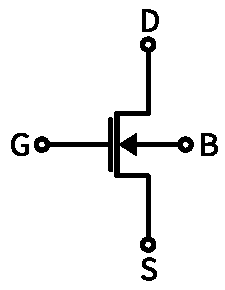
\includegraphics{index_files/mediabag/index_files/figure-pdf/fig-nmos-symbol-output-1.pdf}

}

\caption{\label{fig-nmos-symbol}Circuit symbol of n-channel MOSFET.}

\end{figure}%

\textsubscript{Source:
\href{https://iic-jku.github.io/analog-circuit-design/index.qmd.html}{Article
Notebook}}

\begin{figure}[H]

\centering{

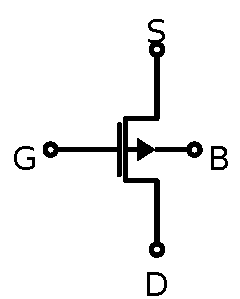
\includegraphics{index_files/mediabag/index_files/figure-pdf/fig-pmos-symbol-output-1.pdf}

}

\caption{\label{fig-pmos-symbol}Circuit symbol of p-channel MOSFET.}

\end{figure}%

\textsubscript{Source:
\href{https://iic-jku.github.io/analog-circuit-design/index.qmd.html}{Article
Notebook}}

For hand calculations and theoretical discussions we will use the
following simplified large-signal model, shown in
Figure~\ref{fig-mosfet-large-signal-model}. A current source
\(I_\mathrm{DS}\) models the current flow between drain and source, and
it is controlled by the three control voltages \(V_\mathrm{GS}\),
\(V_\mathrm{DS}\), and \(V_\mathrm{SB}\). Note that in this way (since
\(I_\mathrm{DS}= f(V_\mathrm{DS})\)) also a resistive behavior between D
and S can be modelled. In case that B and S are shorted then simply
\(V_\mathrm{SB} = 0\).

\textsubscript{Source:
\href{https://iic-jku.github.io/analog-circuit-design/index.qmd.html}{Article
Notebook}}

\begin{figure}[H]

\centering{

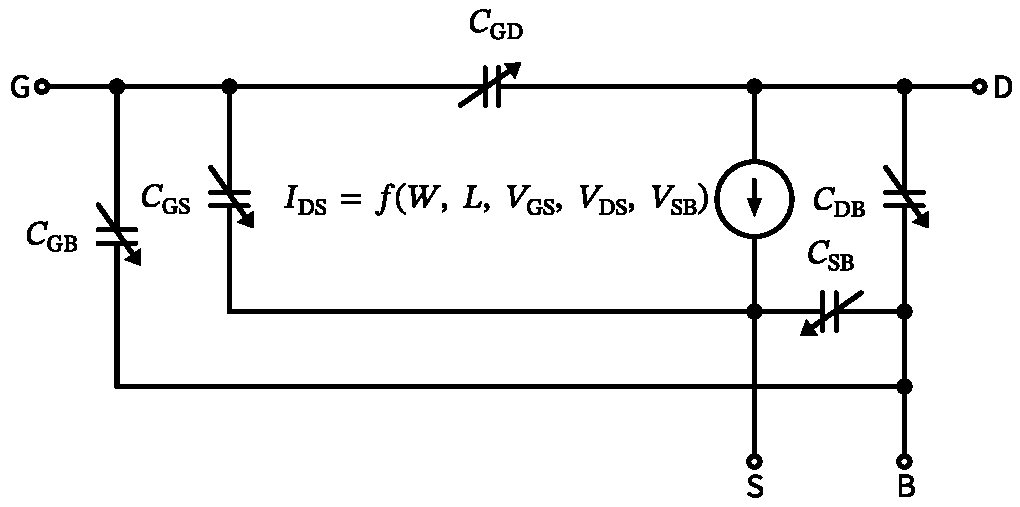
\includegraphics{index_files/mediabag/index_files/figure-pdf/fig-mosfet-large-signal-model-output-1.pdf}

}

\caption{\label{fig-mosfet-large-signal-model}The MOSFET large-signal
model.}

\end{figure}%

\textsubscript{Source:
\href{https://iic-jku.github.io/analog-circuit-design/index.qmd.html}{Article
Notebook}}

In an ideal MOSFET no dc current is flowing into the gate, the behavior
is purely capacitive. We model this by two capacitors:
\(C_\mathrm{GG}= C_\mathrm{GS}+ C_\mathrm{GD}\) is the total capacitance
when looking into the gate of the MOSFET. \(C_\mathrm{GS}\) is usually
the dominant capacitance, and \(C_\mathrm{GD}\) models the capacitive
feedback between D and G, usually induced by a topological overlap
capacitance in the physical construction of the MOSFET. This capacitance
is often small compared to \(C_\mathrm{GS}\), but in situations where we
have a large voltage swing at the drain this capacitance will be
affected by the
\href{https://en.wikipedia.org/wiki/Miller_effect}{Miller effect}. In
hand calculations we will often set \(C_\mathrm{GD}= 0\).

\begin{tcolorbox}[enhanced jigsaw, colback=white, bottomtitle=1mm, titlerule=0mm, toprule=.15mm, coltitle=black, title=\textcolor{quarto-callout-note-color}{\faInfo}\hspace{0.5em}{MOSFET Bulk Terminal}, opacityback=0, leftrule=.75mm, opacitybacktitle=0.6, left=2mm, toptitle=1mm, arc=.35mm, colframe=quarto-callout-note-color-frame, breakable, colbacktitle=quarto-callout-note-color!10!white, rightrule=.15mm, bottomrule=.15mm]

The bulk connection in Figure~\ref{fig-mosfet-large-signal-model} seems
floating as we only consider it a control terminal, where the potential
difference between source and bulk influences the behaviour of the
MOSFET. However, we do not consider resistive or capacitive effects
associated with this node, which is of course a gross simplification,
but nevertheless one we will make in this course.

\end{tcolorbox}

Now, as we are skipping the bottom-up approach of deriving the MOSFET
large-signal behaviour from basic principles, we need to understand the
behaviour of the elements of the large-signal model in
Figure~\ref{fig-mosfet-large-signal-model} by using a circuit simulator
and observing what happens. And generally, a first step in any new IC
technology should be to investigate basic MOSFET performance, by doing
simple dc sweeps of \(V_\mathrm{GS}\) and \(V_\mathrm{DS}\) and looking
at \(I_\mathrm{DS}\) and other large- and small-signal parameters.

As a side note, the students who want to understand MOSFET behaviour
from a physical angle should consult the MOSFET chapter from the JKU
course ``Design of Complex Integrated Circuits'' (VL 336.048). A great
introduction into MOSFET operation and fabrication is given in (Hu
2010), which is available freely
\href{https://www.chu.berkeley.edu/modern-semiconductor-devices-for-integrated-circuits-chenming-calvin-hu-2010/}{online}
and is a recommended read. A very detailed description of the MOSFET
(leaving usually no question unanswered) is provided in (Tsividis and
McAndrew 2011).

Now, in order to get started, basic Xschem testbenches are prepared, and
first simple dc sweeps of various voltages and currents will be done.
But before that, please look at the import note below!

\begin{tcolorbox}[enhanced jigsaw, colback=white, bottomtitle=1mm, titlerule=0mm, toprule=.15mm, coltitle=black, title=\textcolor{quarto-callout-important-color}{\faExclamation}\hspace{0.5em}{Mathematical Notation}, opacityback=0, leftrule=.75mm, opacitybacktitle=0.6, left=2mm, toptitle=1mm, arc=.35mm, colframe=quarto-callout-important-color-frame, breakable, colbacktitle=quarto-callout-important-color!10!white, rightrule=.15mm, bottomrule=.15mm]

Throughout this material, we will largely stick to the following
notation:

\begin{itemize}
\tightlist
\item
  A \textbf{dc quantity} is shown with an upper-case letter with
  upper-case subscripts, like \(V_\mathrm{GS}\).
\item
  Double-subscripts denote \textbf{dc sources}, like \(V_\mathrm{DD}\)
  and \(V_\mathrm{SS}\).
\item
  An \textbf{ac (small-signal) quantity} is a lower-case letter with a
  lower-case subscript, like \(g_\mathrm{m}\).
\item
  A \textbf{total quantity} (dc plus ac) is shown as a lowercase letter
  with upper-case subscript, like \(i_\mathrm{DS}\).
\item
  A upper-case letter with a lower-case subscript is used to denote
  \textbf{RMS quantities}, like \(I_\mathrm{ds}\).
\end{itemize}

\end{tcolorbox}

\subsubsection{Large-Signal MOSFET
Model}\label{large-signal-mosfet-model}

We start with an investigation into the large-signal MOSFET model shown
in Figure~\ref{fig-mosfet-large-signal-model} by using the simple
testbench for the LV NMOS shown in Figure~\ref{fig-simple-nmos-tb}.

\begin{figure}

\centering{

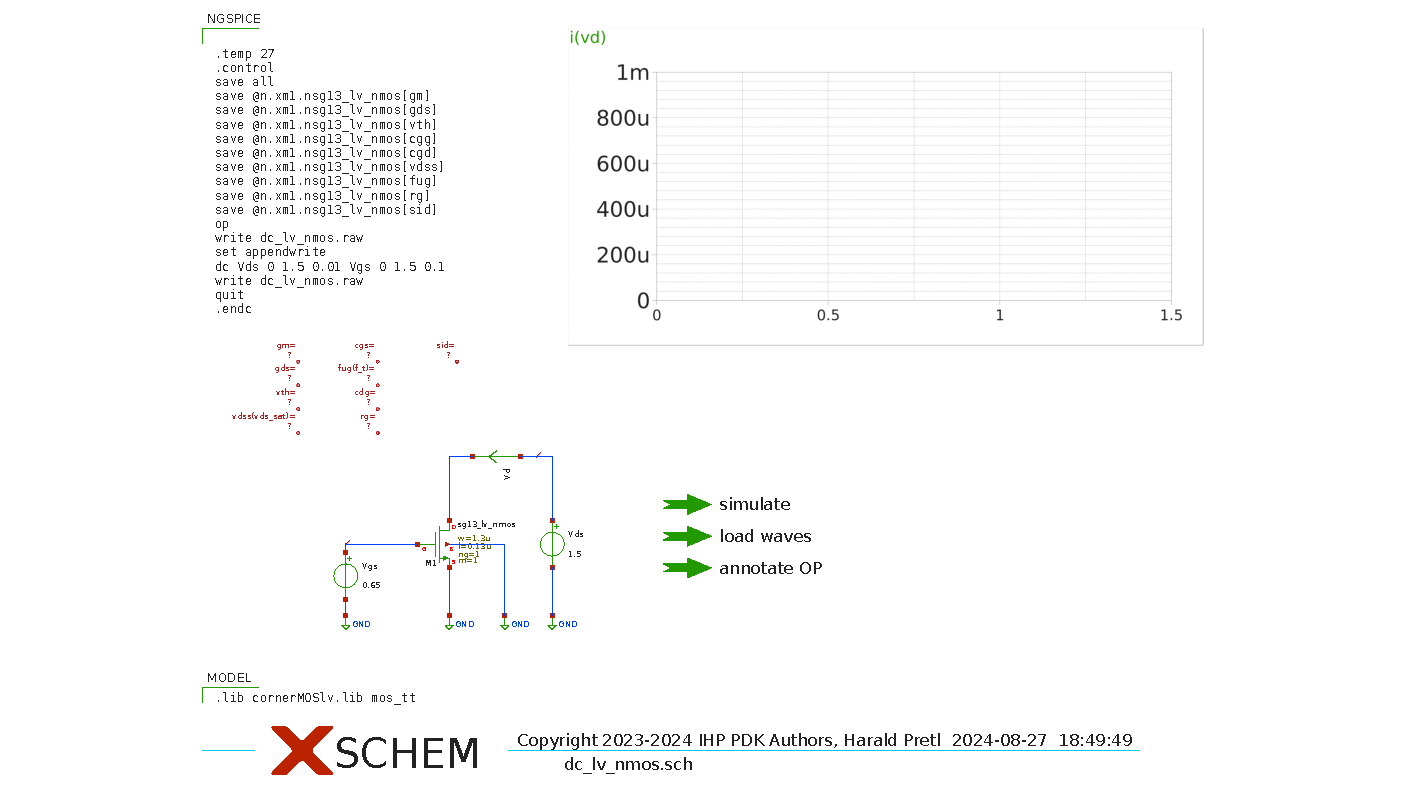
\includegraphics{index_files/mediabag/xschem/dc_lv_nmos.pdf}

}

\caption{\label{fig-simple-nmos-tb}Testbench for NMOS dc sweeps.}

\end{figure}%

\begin{tcolorbox}[enhanced jigsaw, colback=white, bottomtitle=1mm, titlerule=0mm, toprule=.15mm, coltitle=black, title=\textcolor{quarto-callout-tip-color}{\faLightbulb}\hspace{0.5em}{Exercise: MOSFET Investigation}, opacityback=0, leftrule=.75mm, opacitybacktitle=0.6, left=2mm, toptitle=1mm, arc=.35mm, colframe=quarto-callout-tip-color-frame, breakable, colbacktitle=quarto-callout-tip-color!10!white, rightrule=.15mm, bottomrule=.15mm]

Please try to execute the following steps and answer these questions:

\begin{enumerate}
\def\labelenumi{\arabic{enumi}.}
\tightlist
\item
  Get the LV NMOS testbench (available at
  \url{https://github.com/iic-jku/analog-circuit-design/blob/main/xschem/dc_lv_nmos.sch})
  working in your IIC-OSIC-TOOLS environment.
\item
  Make yourself familiar with Xschem (change the schematic in various
  ways, run a simulation, graph the result).
\item
  Make youself familiar with ngspice (run various simulations, save nets
  and parameters, use the embedded Xschem graphing, explore the
  interactive ngspice shell to look at MOSFET model parameters).
\item
  Explore the LV NMOS \texttt{sg13\_lv\_nmos}:

  \begin{enumerate}
  \def\labelenumii{\arabic{enumii}.}
  \tightlist
  \item
    How is \(I_\mathrm{DS}\) affected by \(V_\mathrm{GS}\) and
    \(V_\mathrm{DS}\)?
  \item
    Change \(W\) and \(L\) of the MOSFET. What is the impact on the
    above parameters? Can you explain the variations?
  \item
    When looking at the model parameters in ngspice, you see that there
    is a \(C_\mathrm{GD}\) and a \(C_\mathrm{DG}\). Why is this, what
    could be the difference? Sometimes these capacitors show a negative
    value, why?
  \end{enumerate}
\item
  Build testbenches in Xschem for the LV PMOS, the HV NMOS, and the HV
  PMOS. Explore the different results.

  \begin{enumerate}
  \def\labelenumii{\arabic{enumii}.}
  \tightlist
  \item
    For a given \(W\) and \(L\), which device provides more drain
    current? How are the capacitances related?
  \item
    If you would have to size an inverter, what would be the ideal ratio
    of \(W_p/W_n\)? Will you exactly design this ratio, or are the
    reasons to deviate?
  \item
    There are LV and HV MOSFETs, and you investigated the difference in
    performance. What is the rationale when designing circuits for
    selection either an LV type, and when to choose an HV type?
  \end{enumerate}
\item
  Build a test bench to explore the body effect, start with LV NMOS.

  \begin{enumerate}
  \def\labelenumii{\arabic{enumii}.}
  \tightlist
  \item
    What happens when \(V_\mathrm{BS} \neq 0\)?
  \end{enumerate}
\end{enumerate}

\end{tcolorbox}

\subsubsection{Small-Signal MOSFET
Model}\label{sec-mosfet-smallsignal-model}

As you have seen in the previous investigations, the large-signal model
of Figure~\ref{fig-mosfet-large-signal-model} describes the behaviour of
the MOSFET across a wide range of voltages applied at the MOSFET
terminals. Unfortunately, for hand analysis dealing with a nonlinear
model is close to impossible, at the very least it is quite tedious.

However, for many practical situations, we bias a MOSFET with a set of
dc voltages applied to its terminal, and only apply small signal
excursions during operation. If we do this, we can linearize the
large-signal model in this dc operating point, and resort to a
small-signal model which can be very useful for hand calculations. Many
experienced designers analyze their circuits by doing these kind of hand
calculations and describing the circuit analytically, which is a great
way to understand fundamental performance limits and relationships
between parameters.

We will use the small-signal MOSFET model shown in
Figure~\ref{fig-mosfet-small-signal-model} for this course. The
current-source \(i_\mathrm{ds}= g_\mathrm{m}v_\mathrm{gs}\) models the
drain current as a function of \(v_\mathrm{gs}\), and the resistor
\(g_\mathrm{ds}\) models the dependency of the drain current by
\(v_\mathrm{ds}\). The drain current dependency on the source-bulk
voltage (the so-called ``body effect'') is introduced by the current
source \(i_\mathrm{ds}= g_\mathrm{mb} v_\mathrm{sb}\).

\textsubscript{Source:
\href{https://iic-jku.github.io/analog-circuit-design/index.qmd.html}{Article
Notebook}}

\begin{figure}[H]

\centering{

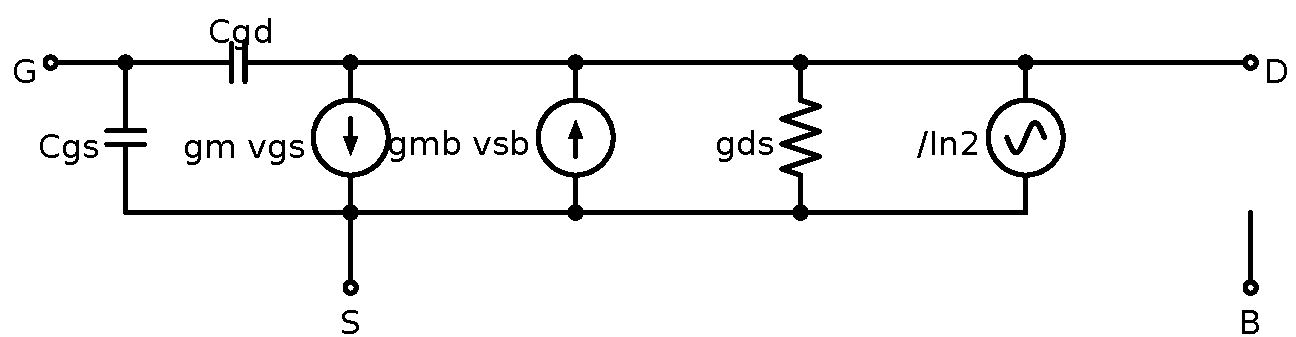
\includegraphics{index_files/mediabag/index_files/figure-pdf/fig-mosfet-small-signal-model-output-1.pdf}

}

\caption{\label{fig-mosfet-small-signal-model}The MOSFET small-signal
model.}

\end{figure}%

\textsubscript{Source:
\href{https://iic-jku.github.io/analog-circuit-design/index.qmd.html}{Article
Notebook}}

As any electronic device the MOSFET introduces noise into the circuit.
In this course we will only consider the drain-source current noise of
the MOSFET, given by
\begin{equation}\phantomsection\label{eq-mosfet-noise}{
\overline{I_\mathrm{n}^2} = 4 k T \gamma g_\mathrm{d0},
}\end{equation} where \(\overline{I_\mathrm{n}^2}\) is the
power-spectral density of the noise in A\(^2\)/Hz; \(k\) is the
Boltzmann constant; \(T\) is the absolute temperature; \(\gamma\) is a
parameter in simplified theory changing between \(\gamma = 2/3\) in
saturation and \(\gamma =1\) for triode operation; \(g_\mathrm{d0}\) is
equal to \(g_\mathrm{m}\) in saturation and \(g_\mathrm{ds}\) in
triode).

\begin{tcolorbox}[enhanced jigsaw, colback=white, bottomtitle=1mm, titlerule=0mm, toprule=.15mm, coltitle=black, title=\textcolor{quarto-callout-note-color}{\faInfo}\hspace{0.5em}{MOSFET Triode and Saturation Region}, opacityback=0, leftrule=.75mm, opacitybacktitle=0.6, left=2mm, toptitle=1mm, arc=.35mm, colframe=quarto-callout-note-color-frame, breakable, colbacktitle=quarto-callout-note-color!10!white, rightrule=.15mm, bottomrule=.15mm]

Sometimes we will refer to different operating modes of the MOSFET like
``saturation'' or ``triode''. Generally speaking, when the drain-source
voltage is small, then the MOSFET acts as a resistor, and this mode of
operation we call ``triode'' mode. When the drain-source voltage is
increased, at some point the drain-source current saturates and is no
longer a strong function of the drain-source voltage. This mode is
called ``saturation'' mode. As you can see in the large-signal
investigations, these transitions happen gradually, and it is difficult
to define a precise point where one operating mode switches to the other
one. In this sense we use terms like ``triode'' and ``saturation'' only
in an approximative sense.

\end{tcolorbox}

Now we need to see how the small-signal parameters seen in
Figure~\ref{fig-mosfet-small-signal-model} can be investigated and
estimated using circuit simulation.

\begin{tcolorbox}[enhanced jigsaw, colback=white, bottomtitle=1mm, titlerule=0mm, toprule=.15mm, coltitle=black, title=\textcolor{quarto-callout-tip-color}{\faLightbulb}\hspace{0.5em}{Exercise: MOSFET Small-Signal Parameters}, opacityback=0, leftrule=.75mm, opacitybacktitle=0.6, left=2mm, toptitle=1mm, arc=.35mm, colframe=quarto-callout-tip-color-frame, breakable, colbacktitle=quarto-callout-tip-color!10!white, rightrule=.15mm, bottomrule=.15mm]

Please try to execute the following steps and answer the following
questions:

\begin{enumerate}
\def\labelenumi{\arabic{enumi}.}
\tightlist
\item
  Reuse the LV NMOS testbench (available at
  \url{https://github.com/iic-jku/analog-circuit-design/blob/main/xschem/dc_lv_nmos.sch}).
\item
  Explore the LV NMOS \texttt{sg13\_lv\_nmos}:

  \begin{enumerate}
  \def\labelenumii{\arabic{enumii}.}
  \tightlist
  \item
    How are \(g_\mathrm{m}\) and \(g_\mathrm{ds}\) changing when you
    change the dc node voltages?
  \item
    What is the ratio of \(g_\mathrm{m}\) to \(g_\mathrm{mb}\)? What is
    the physical reason behind this ratio (you might want to revisit
    MOSFET device physics at this point)?
  \item
    Take a look at the device capacitances \(C_\mathrm{gs}\) and
    \(C_\mathrm{gd}\). Why are they important? What is the relation to
    \(f_\mathrm{T}\)? \emph{Note: \(f_\mathrm{T}\) is the transit
    frequency where the current gain of the MOSFET drops to 1, and can
    be approximated by
    \(2 \pi f_\mathrm{T} = g_\mathrm{m}/ C_\mathrm{gg}\).}
  \item
    Look at the drain noise current according to the MOSFET model and
    compare with a hand calculation of the noise. In the noise equation
    there is the factor \(\gamma\), which in triode is \(\gamma=1\) and
    in saturation is \(\gamma=2/3\) according to basic text books. Which
    value of \(\gamma\) are you calculating? Why might it be different?
  \end{enumerate}
\item
  Go back to your testbench for the LVS PMOS \texttt{sg13\_lv\_pmos}:

  \begin{enumerate}
  \def\labelenumii{\arabic{enumii}.}
  \tightlist
  \item
    What is the difference in \(g_\mathrm{m}\), \(g_\mathrm{ds}\), and
    other parameters between the NMOS and the PMOS? Why could they be
    different?
  \end{enumerate}
\end{enumerate}

\end{tcolorbox}

\subsection{Conclusion}\label{conclusion}

Congratulations for making it thus far! By now you should have a solid
grasp of the tool handling of Xschem and ngspice, and you should be
familiar with the large- and small-signal operation of both NMOS and
PMOS, and the parameters describing these behaviours. If you feel you
are not sufficiently fluent in these things, please go back to the
beginning of Section~\ref{sec-mosfet} and revisit the relevant sections,
or dive into further reading about the MOSFET operation, like in (Hu
2010).

\section{Transistor Sizing Using gm/ID
Methodology}\label{sec-gmid-method}

When designing integrated circuits it is an important question how to
select various parameters of a MOSFET, like \(W\), \(L\), or the bias
current \(I_\mathrm{D}\). In comparison to using discrete components in
PCB design, or also compared to a bipolar junction transistor (BJT), we
have these degrees of freedom, which make integrated circuit design so
interesting.

Often, transistor sizing in entry-level courses is based on the
square-law model, where a simple analytical equation for the drain
current can be derived. However, in nanometer CMOS, the MOSFET behaviour
is much more complex than these simple models. Also, this highly
simplified derivations introduce concepts like the threshold voltage or
the overdrive voltage, which are interesting from a theoretical
viewpoint, but bear little practical use.

\begin{tcolorbox}[enhanced jigsaw, colback=white, bottomtitle=1mm, titlerule=0mm, toprule=.15mm, coltitle=black, title=\textcolor{quarto-callout-note-color}{\faInfo}\hspace{0.5em}{MOSFET Square-Law Model}, opacityback=0, leftrule=.75mm, opacitybacktitle=0.6, left=2mm, toptitle=1mm, arc=.35mm, colframe=quarto-callout-note-color-frame, breakable, colbacktitle=quarto-callout-note-color!10!white, rightrule=.15mm, bottomrule=.15mm]

One of the many simplifactions of the square-law model is that the
mobility of the charge carriers is assumed constant (it is not).
Further, the existance of a threshold voltage is assumed, but in fact
this voltage is just existing given a certain definition, and depending
on definition, its value changed. In addition, in nm CMOS, the threshold
voltage is a function on many thing, like \(W\) and \(L\).

\end{tcolorbox}

An additional shortcoming of the square-law model is that it is only
valid in strong inversion, i.e.~for large \(V_\mathrm{GS}\) where the
drain current is dominated by the drift current. As soon as the
gate-source voltage gets smaller, the square-law model breaks, as the
drain current component based on diffusion currents gets dominant.
Modern compact MOSFET models (like the PSP model used in SG13G2) use
hundreds of parameters and fairly complex equations to somewhat properly
describe MOSFET behaviour over a wide range of parameters like \(W\),
\(L\), and temperature. A modern approach to MOSFET sizing is thus based
on the thought to use exactly these MOSFET models, characterize them,
put the resulting data into tables and charts, and thus learn about the
complext MOSFET behaviour and use it for MOSFET sizing.

Being a well-established approach we select the
\(g_\mathrm{m}/I_\mathrm{D}\) methodology introduced by P. Jespers and
B. Murmann in (Jespers and Murmann 2017). A brief introduction is
available
\href{https://github.com/iic-jku/analog-circuit-design/blob/main/sizing/Ref_Murmann_gmID.pdf}{here}
as well.

The \(g_\mathrm{m}/I_\mathrm{D}\) methodology has the huge advantage
that is catches MOSFET behavior quite accurately over a wide range of
operating conditions, and the curves look very similar for pretty much
all CMOS technologies, form micrometer bulk CMOS down to nanometer
FinFET devices. Of course the absolute values change, but the method
applies universally.

\subsection{MOSFET Characterization
Testbench}\label{mosfet-characterization-testbench}

In order to get the required tabulated data we use a testbench in Xschem
which sweeps the terminal voltages, and records various large- and
small-signal parameters, which are then stored in large tables. The
testbench for the LV NMOS is shown in
Figure~\ref{fig-techsweep-nmos-tb}, and the TB for the LV PMOS is shown
in Figure~\ref{fig-techsweep-pmos-tb}.

\begin{figure}

\centering{

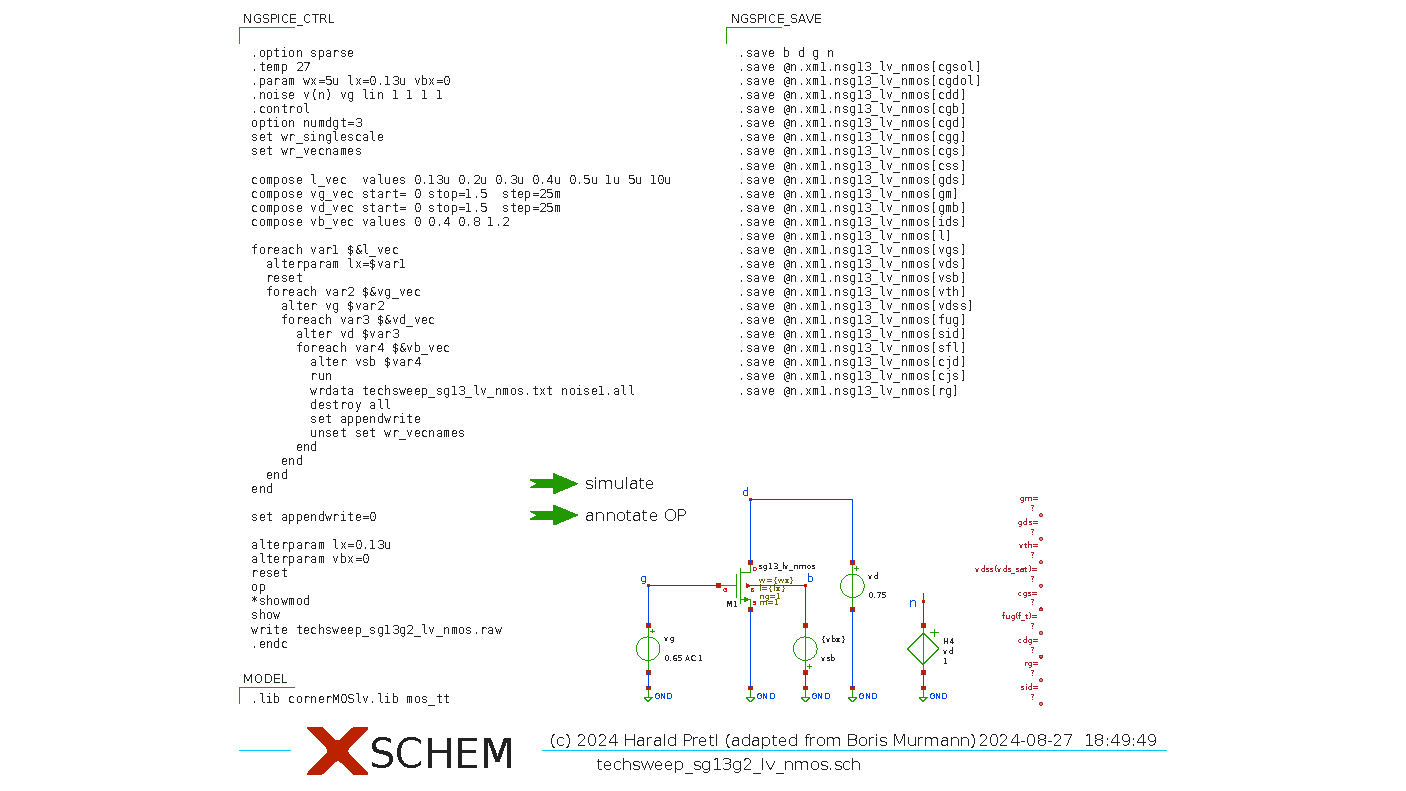
\includegraphics{index_files/mediabag/xschem/techsweep_sg13g2_lv_nmos.pdf}

}

\caption{\label{fig-techsweep-nmos-tb}Testbench for LV NMOS
\(g_\mathrm{m}/I_\mathrm{D}\) characterization.}

\end{figure}%

\begin{figure}

\centering{

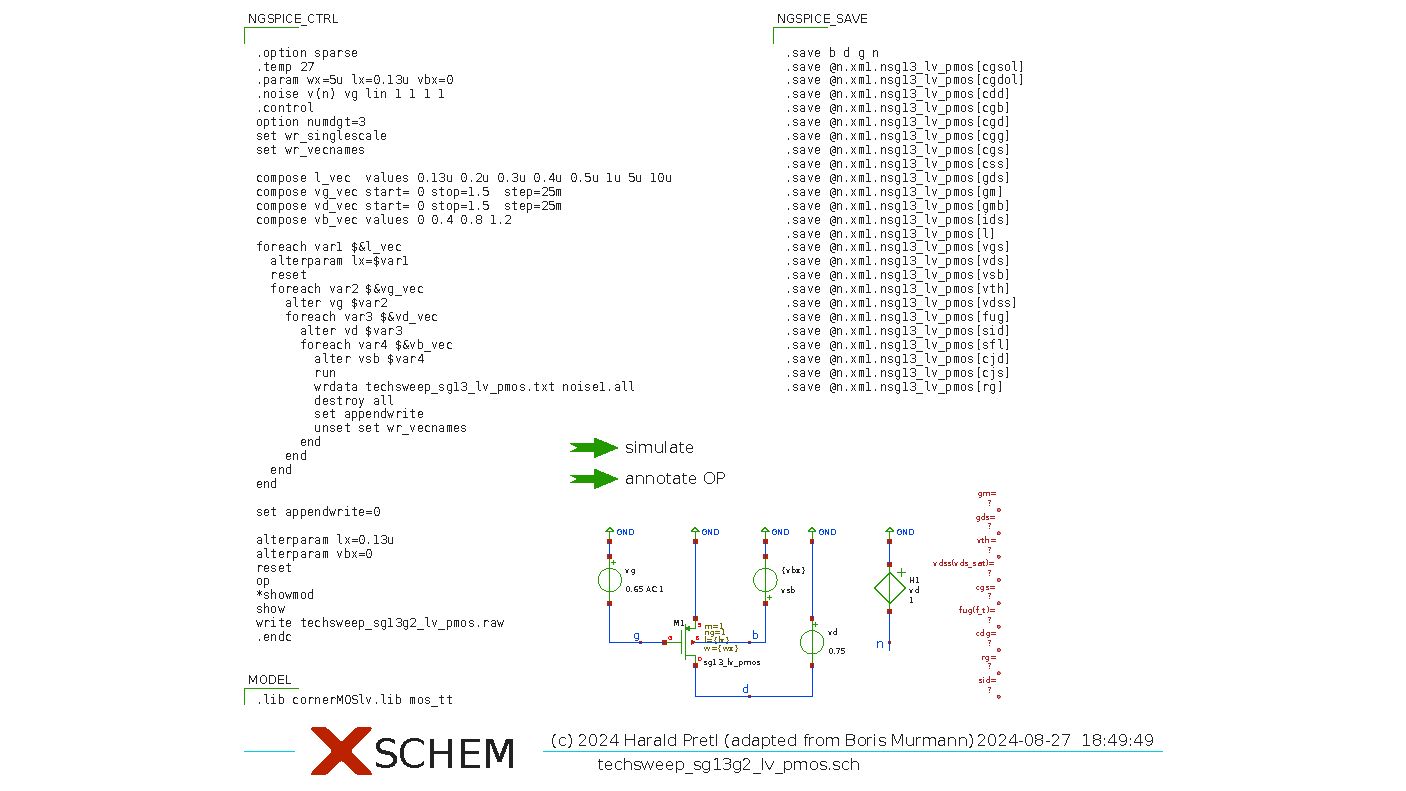
\includegraphics{index_files/mediabag/xschem/techsweep_sg13g2_lv_pmos.pdf}

}

\caption{\label{fig-techsweep-pmos-tb}Testbench for LV PMOS
\(g_\mathrm{m}/I_\mathrm{D}\) characterization.}

\end{figure}%

We will use Jupyter notebooks to inspect the resulting data, and
interpret some important graphs. This will greatly help to understand
the MOSFET behaviour.

\subsection{NMOS Characterization}\label{sec-techsweep-nmos}

First, we will start looking at the LV NMOS. In
Section~\ref{sec-techsweep-pmos} we have the corresponding graphs for
the LV PMOS. In this lecture, we will only use the LV MOSFETs. While
there are also the HV types available, they are mainly used for
high-voltage circuits, like circuits connecting to the outside world.
Here, we only will design low-voltage circuits running at a nominal
supply voltage of \(1.5\,\text{V}\), so only the LV types are of
interest to us.

The first import graph is the plot of \(g_\mathrm{m}/I_\mathrm{D}\) and
\(f_\mathrm{T}\) versus the gate-source voltage \(V_\mathrm{GS}\). First
let us answer the question why \(g_\mathrm{m}/I_\mathrm{D}\) is a good
parameter to look at, and actually this is also the central parameter in
the \(g_\mathrm{m}/I_\mathrm{D}\) methodology. In many circuits that are
biased in class-A (i.e., with a constant quiescent current that is
larger than the largest signal excursion, see
\href{https://en.wikipedia.org/wiki/Power_amplifier_classes\#Class_A}{biasing})
we want to get a large amplification from a MOSFET, which corresponds to
a large \(g_\mathrm{m}\). We want this by spending the minimum biasing
current possible (ideally zero), as we always design for minimum power
consumption. Thus, a high \(g_\mathrm{m}/I_\mathrm{D}\) ratio is good.

\begin{tcolorbox}[enhanced jigsaw, colback=white, bottomtitle=1mm, titlerule=0mm, toprule=.15mm, coltitle=black, title=\textcolor{quarto-callout-note-color}{\faInfo}\hspace{0.5em}{Power Consumption}, opacityback=0, leftrule=.75mm, opacitybacktitle=0.6, left=2mm, toptitle=1mm, arc=.35mm, colframe=quarto-callout-note-color-frame, breakable, colbacktitle=quarto-callout-note-color!10!white, rightrule=.15mm, bottomrule=.15mm]

Designing for minimum power consumption is pretty much always mandated.
For battery-operated equipment it is a paramount requirement, but also
in other equipment electrical energy consumption is a concern, and often
severly limited by the cooling capabilities of the electrical system.

\end{tcolorbox}

However, as can be seen in the below plot, there exists a strong and
unfortunate trade-off with device speed, characterized here by the
transit frequency \(f_\mathrm{T}\). It would be ideal if there exists a
design point where we get high transconductance per bias current
concurrently to having the fastest operation, but unfortunately, this is
clearly not the case. The \(g_\mathrm{m}/I_\mathrm{D}\) peaks for
\(V_\mathrm{GS}< 0.3\,\text{V}\), and the highest speed we get at
\(V_\mathrm{GS}\approx 1.2\,\text{V}\). The dashed vertical line plots
the nominal threshold voltage, as you can see in this continuum of
parameter space, it marks not a particularly special point.

Note that
\begin{equation}\phantomsection\label{eq-mosfet-gmid-weakinversion}{
\frac{g_\mathrm{m}}{I_\mathrm{D}} = \frac{1}{n V_\mathrm{T}}
}\end{equation} for a MOSFET in weak inversion (i.e., small gate-source
voltage). \(n\) is the subthreshold slope, and
\(V_\mathrm{T} = k T / q\) which is \(25.8\,\text{mV}\) at
\(300\,\text{K}\). We thus have \(n \approx 1.38\) for this LV NMOS,
which falls nicely into the usual range for \(n\) of \(1.3\) to \(1.5\)
for bulk CMOS (FinFET have \(n\) very close to \(1\)).

For the classical square-law model of the MOSFET in strong inversion,
\(g_\mathrm{m}/I_\mathrm{D}\) is given as
\begin{equation}\phantomsection\label{eq-mosfet-gmid-stronginversion}{
\frac{g_\mathrm{m}}{I_\mathrm{D}} = \frac{2}{V_\mathrm{GS}- V_\mathrm{th}} = \frac{2}{V_\mathrm{od}} 
}\end{equation} with \(V_\mathrm{th}\) the threshold voltage and
\(V_\mathrm{od}\) the so-called ``overdrive voltage.''

\begin{tcolorbox}[enhanced jigsaw, colback=white, bottomtitle=1mm, titlerule=0mm, toprule=.15mm, coltitle=black, title=\textcolor{quarto-callout-note-color}{\faInfo}\hspace{0.5em}{Why 300K?}, opacityback=0, leftrule=.75mm, opacitybacktitle=0.6, left=2mm, toptitle=1mm, arc=.35mm, colframe=quarto-callout-note-color-frame, breakable, colbacktitle=quarto-callout-note-color!10!white, rightrule=.15mm, bottomrule=.15mm]

Why are we so often using a temperature of \(300\,\text{K}\) for a
typical condition? As this corresponds to roughly
\(27^{\circ}\text{C}\), this accounts for some self heating compared to
otherwise cooler usual room temperatures. Further, engineers like round
numbers which are easy to remember, so \(300\,\text{K}\) is used as a
proxy for room temperature.

\end{tcolorbox}

As we can also see from belows plot, the peak transit frequency of the
LV NMOS is about \(75\,\text{GHz}\), which allows building
radio-frequency circuits up to ca.
\(f_\mathrm{T} / 10 = 7.5\,\text{GHz}\), which is a respectible number.
It is no coincidence, that the transition for RF design in the GHz-range
switched from BJT-based technologies to CMOS roughly in the timeframe
when 130nm CMOS became available (ca. 2000).

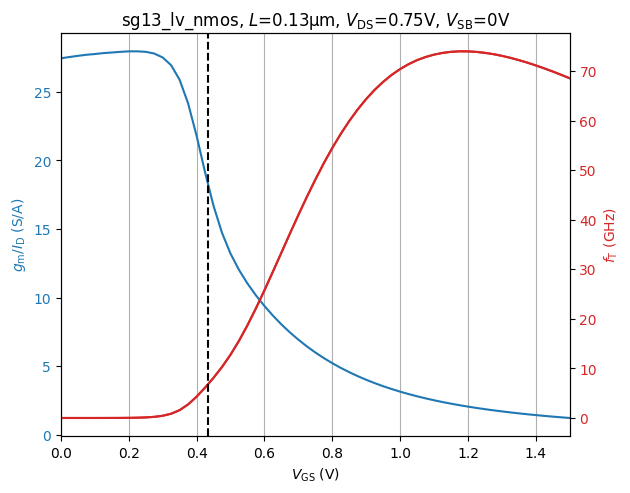
\includegraphics{index_files/figure-latex/.-sizing-techsweep_sg13_plots_nmos-cell-6-output-1.png}

\textsubscript{Source:
\href{https://iic-jku.github.io/analog-circuit-design/index.qmd.html}{Article
Notebook}}

The following figure plots \(f_\mathrm{T}\) against
\(g_\mathrm{m}/I_\mathrm{D}\) for several different \(L\). As you can
see, device speeds maximizes for a low \(g_\mathrm{m}/I_\mathrm{D}\) and
a short \(L\). As you can see the drain-source voltage is kept at
\(V_\mathrm{DS}= 0.75\,\text{V} = V_\mathrm{DD}/ 2\), which is a typical
value keeping the MOSFET in saturation across the characterization
sweeps. Further, the source-bulk voltage is kept at
\(V_\mathrm{SB} = 0\,\text{V}\), which means bulk and source terminals
are connected.

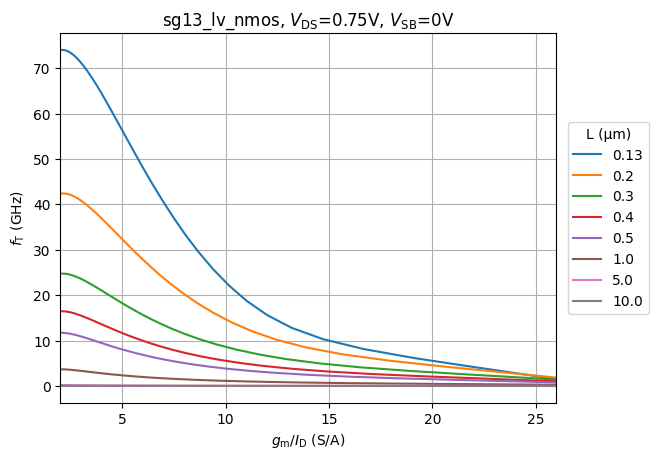
\includegraphics{index_files/figure-latex/.-sizing-techsweep_sg13_plots_nmos-cell-9-output-1.png}

\textsubscript{Source:
\href{https://iic-jku.github.io/analog-circuit-design/index.qmd.html}{Article
Notebook}}

The next plot shows the ratio of \(g_\mathrm{m}/ g_\mathrm{ds}\) versus
\(g_\mathrm{m}/I_\mathrm{D}\). The ratio \(g_\mathrm{m}/ g_\mathrm{ds}\)
is the so-called \textbf{``self-gain''} of the MOSFET, and shows the
maximum voltage gain we can achieve in a single transistor
configuration. As one can see the self gain increases for increasing
\(L\), but this also gives a slower transistor, so again there is a
trade-off. This plot allows us to select the proper \(L\) of a MOSFET if
we know which amount of self gain we need.

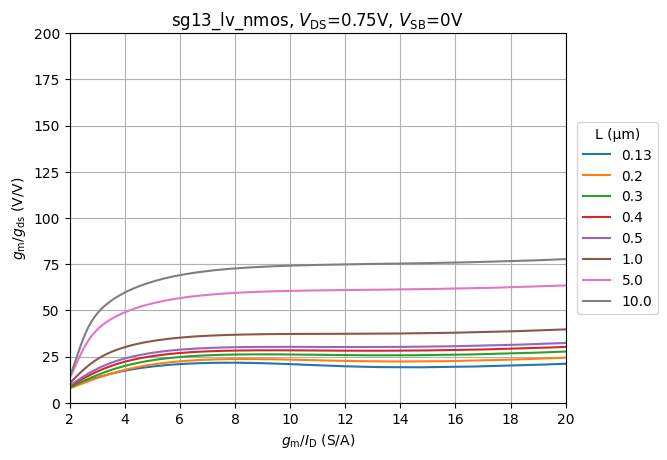
\includegraphics{index_files/figure-latex/.-sizing-techsweep_sg13_plots_nmos-cell-10-output-1.png}

\textsubscript{Source:
\href{https://iic-jku.github.io/analog-circuit-design/index.qmd.html}{Article
Notebook}}

The following figure plots the drain current density \(I_\mathrm{D}/W\)
as a function of \(g_\mathrm{m}/I_\mathrm{D}\) and \(L\). With this plot
we can find out how to set the \(W\) of a MOSFET once we know the
biasing current \(I_\mathrm{D}\), the \(L\) (selected according to self
gain, \(f_\mathrm{T}\), and other considerations) and the
\(g_\mathrm{m}/I_\mathrm{D}\) design point we selected. The drain
current density \(I_\mathrm{D}/W\) is a very useful nomalized metric to
use, because the physical action in the MOSFET establishes a charge
density in the channel below the gate, and the changing of the \(W\) of
the device merely transforms this charge density into an absolute
parameter (together with \(L\)).

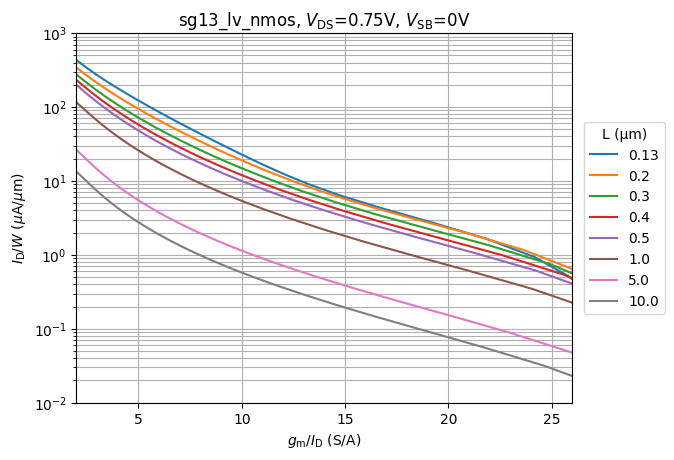
\includegraphics{index_files/figure-latex/.-sizing-techsweep_sg13_plots_nmos-cell-11-output-1.png}

\textsubscript{Source:
\href{https://iic-jku.github.io/analog-circuit-design/index.qmd.html}{Article
Notebook}}

The following plot shows the minimum drain-source voltage
\(V_\mathrm{ds,sat}\) that we need to establish in order to keep the
MOSFET in saturation. As you can see, this value is almost independent
of \(L\), and increases for small \(g_\mathrm{m}/I_\mathrm{D}\). So for
low-voltage circuits, where headroom is precious, we tend to bias at
\(g_\mathrm{m}/I_\mathrm{D}\ge 10\), wheres for fast circuits we need to
go to small \(g_\mathrm{m}/I_\mathrm{D}\le 5\) requiring substantial
voltage headroom per MOSFET stage that we stack on top of each other.

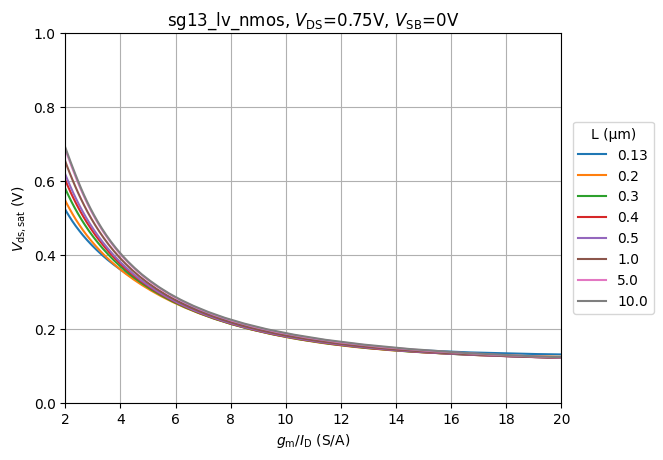
\includegraphics{index_files/figure-latex/.-sizing-techsweep_sg13_plots_nmos-cell-12-output-1.png}

\textsubscript{Source:
\href{https://iic-jku.github.io/analog-circuit-design/index.qmd.html}{Article
Notebook}}

For analog circuits the noise performance is usually quite important.
Thermal noise of a resistor (the Johnson-Nyquist noise) has a flat
power-spectral density (PSD) given by
\(\overline{V_\mathrm{n}^2}/\Delta f = 4 k T R\), where \(k\) is
Boltzmann's constant, \(T\) absolute temperature, and \(R\) the value of
the resistor (the unit of \(\overline{V_\mathrm{n}^2}/\Delta f\) is
\(\text{V}^2/\text{Hz}\)). This PSD is essentially flat until very high
frequencies where
\href{https://en.wikipedia.org/wiki/Johnson–Nyquist_noise}{quantum
effects} start to kick in.

\begin{tcolorbox}[enhanced jigsaw, colback=white, bottomtitle=1mm, titlerule=0mm, toprule=.15mm, coltitle=black, title=\textcolor{quarto-callout-note-color}{\faInfo}\hspace{0.5em}{Noise Notation}, opacityback=0, leftrule=.75mm, opacitybacktitle=0.6, left=2mm, toptitle=1mm, arc=.35mm, colframe=quarto-callout-note-color-frame, breakable, colbacktitle=quarto-callout-note-color!10!white, rightrule=.15mm, bottomrule=.15mm]

We usually leave the \(\Delta f\) away for a shorter notation, so we
write \(\overline{V_\mathrm{n}^2}\) when we actually mean
\(\overline{V_\mathrm{n}^2}/\Delta f\). In case of doubt look at the
unit of a quantity, whether is shows \(\text{V}^2\) or
\(\text{V}^2/\text{Hz}\) or \(\text{V}/\sqrt{\text{Hz}}\) (or
\(\text{I}^2\) or \(\text{I}^2/\text{Hz}\) or
\(\text{I}/\sqrt{\text{Hz}}\)).

Please also note that the pair of \(k T\) pretty much always shows up
together, so when you do a calculation and you miss the one or the
other, that is often a sign for miscalculation. Boltzmann's constant
\(k = 1.38 \cdot 10^{-23}\,\text{J/K}\) is just a scaling factor from
thermal energy expressed as a temperature \(T\) to energy \(E = k T\)
expressed in Joule.

Further, when working with PSD there is the usage of a one-sided
(\(0 \ge f < \infty\)) or two-sided power spectral density (PSD)
(\(-\infty < f < \infty\)). The default in this lecture is the usage of
the \textbf{one-sided PSD}.

\end{tcolorbox}

In this lecture the only MOSFET noise we consider is the drain noise (as
discussed in Section~\ref{sec-mosfet-smallsignal-model}), showing up as
a current noise between drain and source. For a for realistic MOSFET
noise model, also a (correlated) gate noise component and the thermal
noise of the gate resistance needs to be considered.

The factor \(\gamma\) (Equation~\ref{eq-mosfet-noise}) is a function of
many things (in classical theory, \(\gamma = 2/3\) in saturation and
\(\gamma = 1\) in triode), and it is characterized in the following plot
as a function of \(g_\mathrm{m}/I_\mathrm{D}\) and \(L\). So when
calculating MOSFET noise we can lookup \(\gamma\) in the below plot, and
use Equation~\ref{eq-mosfet-noise} to calculate the effective drain
current noise.

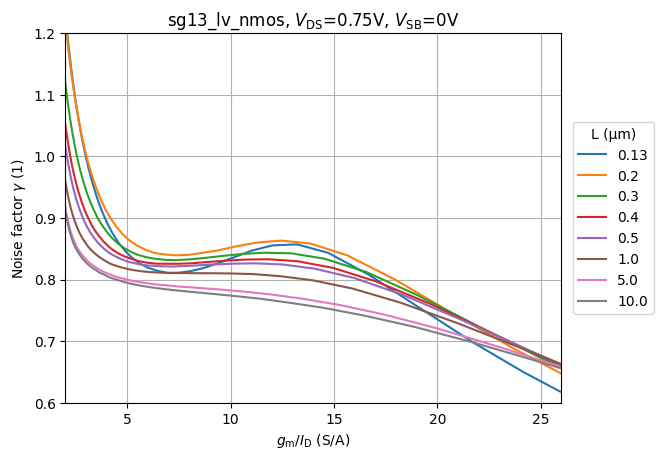
\includegraphics{index_files/figure-latex/.-sizing-techsweep_sg13_plots_nmos-cell-13-output-1.png}

\textsubscript{Source:
\href{https://iic-jku.github.io/analog-circuit-design/index.qmd.html}{Article
Notebook}}

In a MOSFET, unfortunately, besides the thermal noise according to
Equation~\ref{eq-mosfet-noise}, there is also a substantial
low-frequency excess noise, called ``flicker noise'' due to its
characteristic \(\overline{I_\mathrm{d,nf}^2} = K_\mathrm{f}/f\)
behaviour (this means that this noise PSD decreases versus frequency).
In order to characterize this flicker noise the following plot shows the
cross-over frequency \(f_\mathrm{co}\), where the flicker noise is as
large as the thermal noise. As can be seen in the below plot, this
frequency is a strong function of \(L\) and
\(g_\mathrm{m}/I_\mathrm{D}\). Generally, the flicker noise is
proportional to \((W L)^{-1}\), so the larger the device is, the lower
the flicker noise. The parameter \(g_\mathrm{m}/I_\mathrm{D}\) largely
stays constant when we keep \(W/L\) constant, so for a given
\(g_\mathrm{m}/I_\mathrm{D}\) flicker noise is proportinal to \(1/L^2\).
However, increasing \(L\) lowers device speed dramatically, so here we
have a trade-off between flicker-noise performance and MOSFET speed, and
this can have dramatic consequences for high-speed circuits.

\begin{tcolorbox}[enhanced jigsaw, colback=white, bottomtitle=1mm, titlerule=0mm, toprule=.15mm, coltitle=black, title=\textcolor{quarto-callout-note-color}{\faInfo}\hspace{0.5em}{MOSFET Flicker Noise}, opacityback=0, leftrule=.75mm, opacitybacktitle=0.6, left=2mm, toptitle=1mm, arc=.35mm, colframe=quarto-callout-note-color-frame, breakable, colbacktitle=quarto-callout-note-color!10!white, rightrule=.15mm, bottomrule=.15mm]

The physical origin of flicker noise is the crystal interface between
silicon (Si) and the silicondioxide (SiO\textsubscript{2}). Since these
are different materials, there are dangling bonds, which can capture
charge charriers travelling in the channel. After a random time, these
carriers are released, and flicker noise is the result. The amount of
flicker noise is a function of the manufacturing process, and will
generally be different between device types and wafer foundries.

\end{tcolorbox}

As you can see in the following plot, \(f_\mathrm{co}\) can reach well
into the 10's of MHz for short MOSFETs, significantly degrading the
noise performance of a circuit.

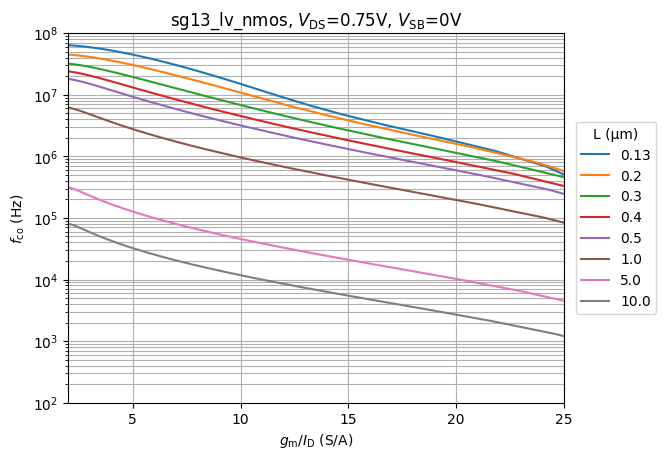
\includegraphics{index_files/figure-latex/.-sizing-techsweep_sg13_plots_nmos-cell-14-output-1.png}

\textsubscript{Source:
\href{https://iic-jku.github.io/analog-circuit-design/index.qmd.html}{Article
Notebook}}

\subsection{PMOS Characterization}\label{sec-techsweep-pmos}

In the following, we have the same plots as discussed in
Section~\ref{sec-techsweep-nmos}, but now for the PMOS.

\begin{tcolorbox}[enhanced jigsaw, colback=white, bottomtitle=1mm, titlerule=0mm, toprule=.15mm, coltitle=black, title=\textcolor{quarto-callout-note-color}{\faInfo}\hspace{0.5em}{PMOS Sign Convention}, opacityback=0, leftrule=.75mm, opacitybacktitle=0.6, left=2mm, toptitle=1mm, arc=.35mm, colframe=quarto-callout-note-color-frame, breakable, colbacktitle=quarto-callout-note-color!10!white, rightrule=.15mm, bottomrule=.15mm]

In all PMOS plots we plot positive values for voltages and currents, to
have compatible plots to the NMOS. Of course, in a PMOS, voltages and
currents have different polarity compared to the NMOS.

\end{tcolorbox}

\(g_\mathrm{m}/I_\mathrm{D}\) and \(f_\mathrm{T}\) versus the
gate-source voltage \(V_\mathrm{GS}\):

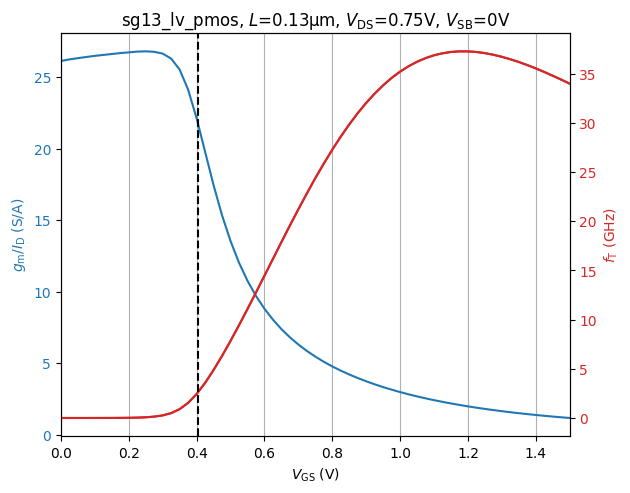
\includegraphics{index_files/figure-latex/.-sizing-techsweep_sg13_plots_pmos-cell-6-output-1.png}

\textsubscript{Source:
\href{https://iic-jku.github.io/analog-circuit-design/index.qmd.html}{Article
Notebook}}

\(f_\mathrm{T}\) against \(g_\mathrm{m}/I_\mathrm{D}\) for several
different \(L\). One can see significantly lower top speed for the PMOS
compared to the NMOS, which means for high-speed circuits the NMOS
should be used.

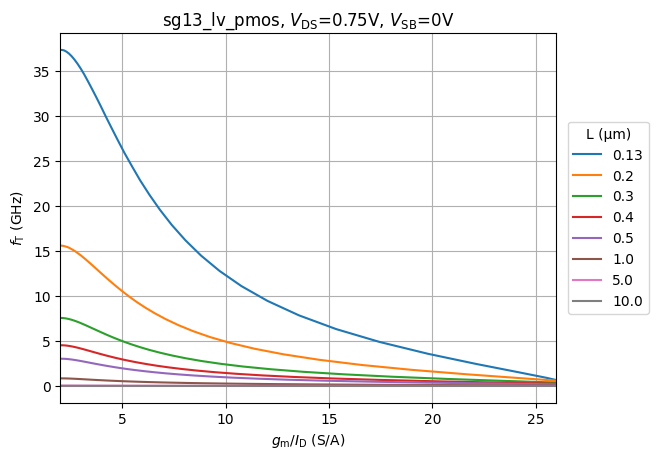
\includegraphics{index_files/figure-latex/.-sizing-techsweep_sg13_plots_pmos-cell-9-output-1.png}

\textsubscript{Source:
\href{https://iic-jku.github.io/analog-circuit-design/index.qmd.html}{Article
Notebook}}

\(g_\mathrm{m}/ g_\mathrm{ds}\) versus \(g_\mathrm{m}/I_\mathrm{D}\).
Unfortunately, one can see a modelling error for the PMOS in this plot.
The self gain \(g_\mathrm{m}/ g_\mathrm{ds}\) reaches non-physical
values, which indicates an issue with the \(g_\mathrm{ds}\) modelling
for the PMOS. We can not use these values for our circuit sizing, so we
will use the respective NMOS plots also for the PMOS.

\begin{tcolorbox}[enhanced jigsaw, colback=white, bottomtitle=1mm, titlerule=0mm, toprule=.15mm, coltitle=black, title=\textcolor{quarto-callout-important-color}{\faExclamation}\hspace{0.5em}{Beware of Modelling Issues}, opacityback=0, leftrule=.75mm, opacitybacktitle=0.6, left=2mm, toptitle=1mm, arc=.35mm, colframe=quarto-callout-important-color-frame, breakable, colbacktitle=quarto-callout-important-color!10!white, rightrule=.15mm, bottomrule=.15mm]

This example shows how important it is to benchmark the device models
when starting to use a new technology. Modelling artifacts like the one
shown are quite often happening, as setting up the device compact models
and parametrizing them according to measurement data is a very complex
task. In any case, just be aware that modelling issues could exist in
whatever PDK you are going to use!

\end{tcolorbox}

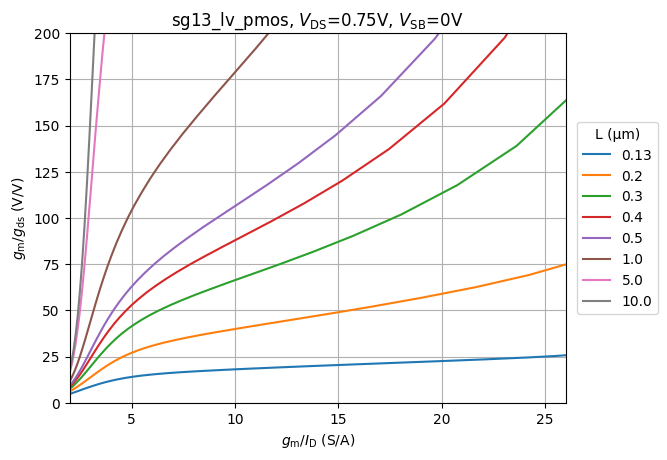
\includegraphics{index_files/figure-latex/.-sizing-techsweep_sg13_plots_pmos-cell-10-output-1.png}

\textsubscript{Source:
\href{https://iic-jku.github.io/analog-circuit-design/index.qmd.html}{Article
Notebook}}

Drain current density \(I_\mathrm{D}/W\) as a function of
\(g_\mathrm{m}/I_\mathrm{D}\) and \(L\):

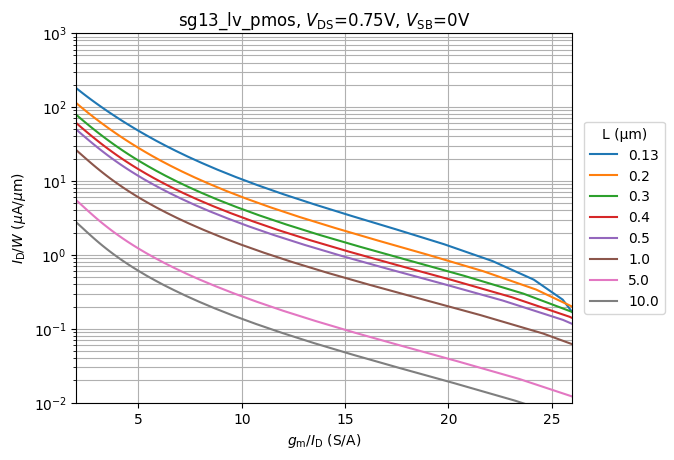
\includegraphics{index_files/figure-latex/.-sizing-techsweep_sg13_plots_pmos-cell-11-output-1.png}

\textsubscript{Source:
\href{https://iic-jku.github.io/analog-circuit-design/index.qmd.html}{Article
Notebook}}

Minimum drain-source voltage \(V_\mathrm{ds,sat}\) versus
\(g_\mathrm{m}/I_\mathrm{D}\) and \(L\):

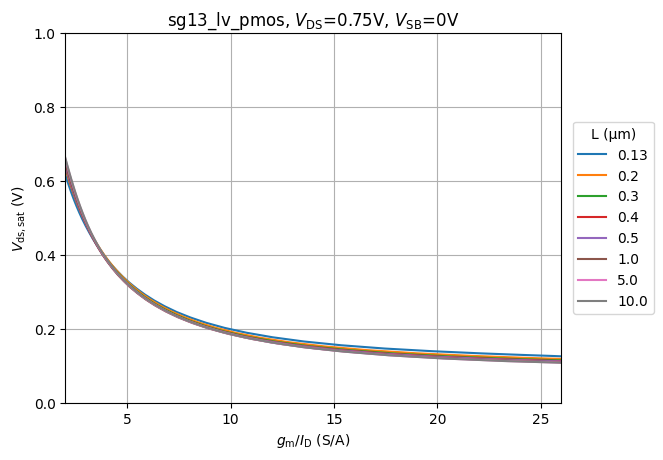
\includegraphics{index_files/figure-latex/.-sizing-techsweep_sg13_plots_pmos-cell-12-output-1.png}

\textsubscript{Source:
\href{https://iic-jku.github.io/analog-circuit-design/index.qmd.html}{Article
Notebook}}

Noise factor \(\gamma\) versus \(g_\mathrm{m}/I_\mathrm{D}\) and \(L\):

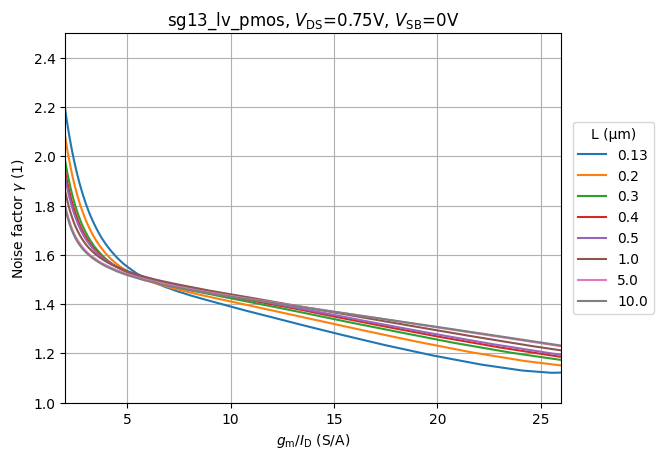
\includegraphics{index_files/figure-latex/.-sizing-techsweep_sg13_plots_pmos-cell-13-output-1.png}

\textsubscript{Source:
\href{https://iic-jku.github.io/analog-circuit-design/index.qmd.html}{Article
Notebook}}

Flicker noise corner frequency \(f_\mathrm{co}\) versus
\(g_\mathrm{m}/I_\mathrm{D}\) and \(L\). If you compare this figure
carefully with the NMOS figure you can see that for some operating
points the flicker noise for the PMOS is lower than for the NMOS. This
is often true for CMOS technologies, so it can be an advantage to use a
PMOS transistor in places where flicker noise is critical, like an OTA
input stage. Using PMOS has the further advantage that the bulk node can
be tied to source (which for NMOS is only possible in a triple-well
technology, which is often not available), which gets rid of the
\href{https://en.wikipedia.org/wiki/Threshold_voltage}{body effect}.

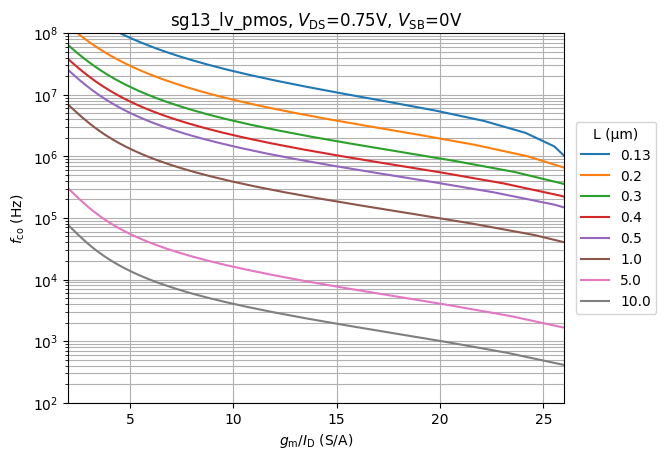
\includegraphics{index_files/figure-latex/.-sizing-techsweep_sg13_plots_pmos-cell-14-output-1.png}

\textsubscript{Source:
\href{https://iic-jku.github.io/analog-circuit-design/index.qmd.html}{Article
Notebook}}

\section{First Circuit: MOSFET Diode}\label{sec-mosfet-diode}

The first (simple) circuit we will investigate is a MOSFET, where the
gate is shorted with a drain, a so-called MOSFET ``diode'', which is
shown in Figure~\ref{fig-mosfet-diode}. This diode is one half of a
current mirror, which we will investigate in a future section.

\textsubscript{Source:
\href{https://iic-jku.github.io/analog-circuit-design/index.qmd.html}{Article
Notebook}}

\begin{figure}[H]

\centering{

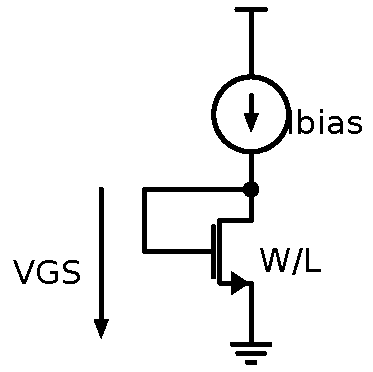
\includegraphics{index_files/mediabag/index_files/figure-pdf/fig-mosfet-diode-output-1.pdf}

}

\caption{\label{fig-mosfet-diode}A MOSFET connected as a diode.}

\end{figure}%

\textsubscript{Source:
\href{https://iic-jku.github.io/analog-circuit-design/index.qmd.html}{Article
Notebook}}

Why looking at a single-transistor circuit at all? By starting with the
simplest possible circuit we can develop important skills in circuit
analysis (setting up and calculating a small-signal model, calculating
open-loop gain, calculate noise) and Xschem/ngspice simulation testbench
creation. We safely assume that also the Mona Lisa was not Leonardo da
Vinci's first painting, so let's start slow.

This diode is usually biased by a current source, shown as
\(I_\mathrm{bias}\) in the figure. Depending on MOSFET sizing with \(W\)
and \(L\), a certain gate-source voltage \(V_\mathrm{GS}\) will develop.
This voltage can be used as a biasing voltage for other circuit parts,
for example.

\begin{tcolorbox}[enhanced jigsaw, colback=white, bottomtitle=1mm, titlerule=0mm, toprule=.15mm, coltitle=black, title=\textcolor{quarto-callout-note-color}{\faInfo}\hspace{0.5em}{Feedback in the MOSFET Diode}, opacityback=0, leftrule=.75mm, opacitybacktitle=0.6, left=2mm, toptitle=1mm, arc=.35mm, colframe=quarto-callout-note-color-frame, breakable, colbacktitle=quarto-callout-note-color!10!white, rightrule=.15mm, bottomrule=.15mm]

It is important to realize that this configuration essentially employs a
feedback loop for operation. The voltage at the drain of the MOSFET is
sensed by the gate, and the gate voltage changes until the
\(I_\mathrm{D}\) is exactly equal to \(I_\mathrm{bias}\). In this sense
this is probably the smallest feedback circuit one can build.

\end{tcolorbox}

\subsection{MOSFET Diode Sizing}\label{mosfet-diode-sizing}

We will now build this circuit in Xschem. For sizing the MOSFET we will
use the \(g_\mathrm{m}/I_\mathrm{D}\) methodology introduced in
Section~\ref{sec-gmid-method}.

\begin{tcolorbox}[enhanced jigsaw, colback=white, bottomtitle=1mm, titlerule=0mm, toprule=.15mm, coltitle=black, title=\textcolor{quarto-callout-tip-color}{\faLightbulb}\hspace{0.5em}{Exercise: MOSFET Diode Sizing}, opacityback=0, leftrule=.75mm, opacitybacktitle=0.6, left=2mm, toptitle=1mm, arc=.35mm, colframe=quarto-callout-tip-color-frame, breakable, colbacktitle=quarto-callout-tip-color!10!white, rightrule=.15mm, bottomrule=.15mm]

Please build a MOSFET diode circuit in Xschem where you use an LV NMOS,
set \(I_\mathrm{bias} = 20\,\mu\text{A}\), \(L = 0.13\,\mu\text{m}\),
and we want to use \(g_\mathrm{m}/I_\mathrm{D}= 10\) (often a suitable
compromise between transistor speed and \(g_\mathrm{m}\) efficiency).

\begin{enumerate}
\def\labelenumi{\arabic{enumi}.}
\tightlist
\item
  Use the figures in Section~\ref{sec-techsweep-nmos} to find out the
  proper value for \(W\).
\item
  What is \(f_\mathrm{T}\) for this MOSFET? What is the value for
  \(g_\mathrm{m}\) and \(g_\mathrm{ds}\)?
\item
  Draw the circuit in Xschem, and simulate the operating point. Do the
  values match to the values found out before during circuit sizing?
\end{enumerate}

\end{tcolorbox}

Before continuing, please finish the previous exercise. Once you are
done, compare with the below provided solution.

\begin{tcolorbox}[enhanced jigsaw, colback=white, bottomtitle=1mm, titlerule=0mm, toprule=.15mm, coltitle=black, title=\textcolor{quarto-callout-tip-color}{\faLightbulb}\hspace{0.5em}{Solution: MOSFET Diode Sizing}, opacityback=0, leftrule=.75mm, opacitybacktitle=0.6, left=2mm, toptitle=1mm, arc=.35mm, colframe=quarto-callout-tip-color-frame, breakable, colbacktitle=quarto-callout-tip-color!10!white, rightrule=.15mm, bottomrule=.15mm]

\begin{enumerate}
\def\labelenumi{\arabic{enumi}.}
\tightlist
\item
  Using the fact that
  \(I_\mathrm{bias} = I_\mathrm{D} = 20\,\mu\text{A}\) and
  \(g_\mathrm{m}/I_\mathrm{D}= 10\) directly provides
  \(g_\mathrm{m}= 0.2\,\text{mS}\).
\item
  Using the self-gain plot, we see that
  \(g_\mathrm{m}/g_\mathrm{ds}\approx 21\), so
  \(g_\mathrm{ds}\approx 9.5\,\mu\text{S}\). The \(f_\mathrm{T}\) can
  easily be found in the respective plot to be
  \(f_\mathrm{T} = 23\,\text{GHz}\).
\item
  The \(W\) of the MOSFET we find using the drain current density plot
  and the given bias current. Rounding to half-microns results in
  \(W = 1\,\mu\text{m}\).
\item
  Since we are looking at the graphs, we further find \(\gamma = 0.84\),
  \(V_\mathrm{ds,sat} = 0.18\,\text{V}\), and
  \(f_\mathrm{co} \approx 15\,\text{MHz}\).
\item
  In addition, we expect \(V_\mathrm{GS}\approx 0.6\,\text{V}\).
\end{enumerate}

An example Jupyter notebook to extract these values accurately you can
find \href{./sizing/sizing_mosfet_diode.ipynb}{here}. An Xschem
schematic for this exercise is provide
\href{./xschem/mosfet_diode_sizing.sch}{as well}.

\end{tcolorbox}

\subsection{MOSFET Diode Large-Signal
Behaviour}\label{mosfet-diode-large-signal-behaviour}

As discussed above, the MOSFET diode configuration is essentially a
feedback loop. Before we will analyse this loop in small-signal, we want
to investgate how this loop settles in the time domain, and by doing
this we can observe the large-signal settling behaviour. To simulate
this, we change the dc bias source from the previous example to a
transient current source, which we will turn on after some ns. The
resulting Xschem testbench is shown in
Figure~\ref{fig-mosfet-diode-settling-tb}.

\begin{figure}

\centering{

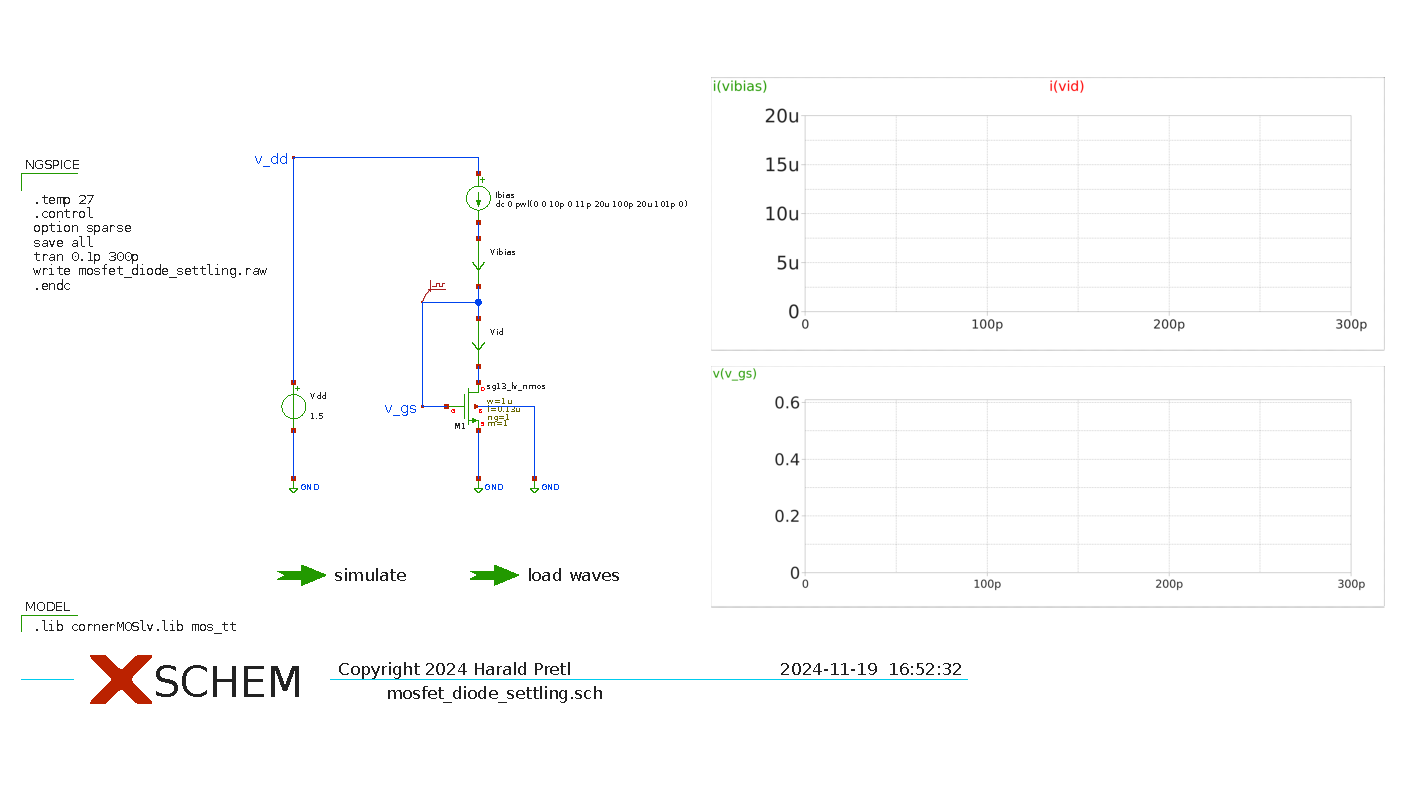
\includegraphics{index_files/mediabag/xschem/mosfet_diode_settling.pdf}

}

\caption{\label{fig-mosfet-diode-settling-tb}Testbench for MOSFET diode
transient settling.}

\end{figure}%

In Figure~\ref{fig-mosfet-diode-settling-tb} another interesting effect
can be observed: While the turn-on happens quite rapidly (essentially
the bias current source charges the gate capacitance, until the
gate-source voltage is large enough that the drain current counteracts
the bias current), the turn-off shows a very long settling tail. This is
due to the fact that as the gate capacitance is discharged by the drain
current the \(V_\mathrm{GS}\) drops, which in turn reduces the drain
current, which will make the discharge even slower. We have an effect
similar to the capacitor discharge by a diode (Hellen 2003).

It is thus generally a good idea to add power-down switches to the
circuits to disable the circuit quickly by pulling floating nodes to a
defined potential (usually \(V_\mathrm{DD}\) or \(V_\mathrm{SS}\)) and
to avoid long intermediate states during power down. This will also
allow a turn-on from a well-defined off-state.

\subsection{MOSFET Diode Small-Signal
Analysis}\label{mosfet-diode-small-signal-analysis}

We now want to investigate the small-signal behaviour of the MOSFET
diode. Based on the small-signal model of the MOSFET in
Figure~\ref{fig-mosfet-small-signal-model} we realize that gate and
drain are shorted, and we also connect bulk to source. We can thus
simplify the circit to the one shown in
Figure~\ref{fig-mosfet-diode-small-signal}.

\textsubscript{Source:
\href{https://iic-jku.github.io/analog-circuit-design/index.qmd.html}{Article
Notebook}}

\begin{figure}[H]

\centering{

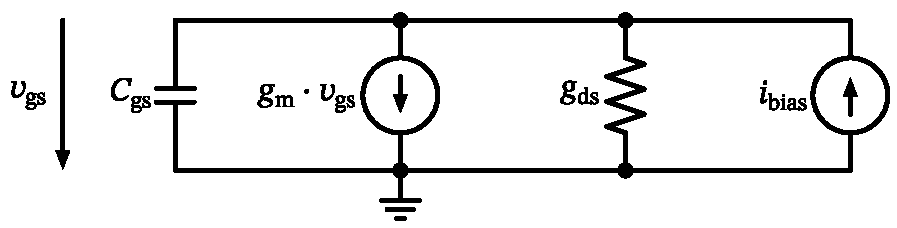
\includegraphics{index_files/mediabag/index_files/figure-pdf/fig-mosfet-diode-small-signal-output-1.pdf}

}

\caption{\label{fig-mosfet-diode-small-signal}The MOSFET diode
small-signal model.}

\end{figure}%

\textsubscript{Source:
\href{https://iic-jku.github.io/analog-circuit-design/index.qmd.html}{Article
Notebook}}

\begin{tcolorbox}[enhanced jigsaw, colback=white, bottomtitle=1mm, titlerule=0mm, toprule=.15mm, coltitle=black, title=\textcolor{quarto-callout-note-color}{\faInfo}\hspace{0.5em}{Ground Node Selection}, opacityback=0, leftrule=.75mm, opacitybacktitle=0.6, left=2mm, toptitle=1mm, arc=.35mm, colframe=quarto-callout-note-color-frame, breakable, colbacktitle=quarto-callout-note-color!10!white, rightrule=.15mm, bottomrule=.15mm]

For small-signal analysis we would not need to declare one node as the
ground potential. However, when doing so, and selecting the ground node
strategically, we can simplify the analysis, as we usually do not
formulate KCL for the ground node (as we have only \(N-1\) independent
KCL equations, \(N\) being the number of nodes in the circuit), and the
potential difference equations are simpler if one node is at \(0\,V\).

\end{tcolorbox}

For calculating the small-signal impedance of the MOSFET diode we
formulate KCL at the top node to get \[
i_\mathrm{bias} - s C_\mathrm{gs}v_\mathrm{gs}- g_\mathrm{m}v_\mathrm{gs}- g_\mathrm{ds}v_\mathrm{gs}= 0.
\]

It follows that
\begin{equation}\phantomsection\label{eq-mosfet-diode-impedance}{
Z_\mathrm{diode}(s) = \frac{v_\mathrm{gs}}{i_\mathrm{bias}} = \frac{1}{g_\mathrm{m}+ g_\mathrm{ds}+ s C_\mathrm{gs}}.
}\end{equation}

When neglecting \(g_\mathrm{ds}\) and at dc we get
\(Z_\mathrm{diode} = 1 / g_\mathrm{m}\), which is an important result
and should be memorized.

\begin{tcolorbox}[enhanced jigsaw, colback=white, bottomtitle=1mm, titlerule=0mm, toprule=.15mm, coltitle=black, title=\textcolor{quarto-callout-important-color}{\faExclamation}\hspace{0.5em}{The Admittance is Your Friend}, opacityback=0, leftrule=.75mm, opacitybacktitle=0.6, left=2mm, toptitle=1mm, arc=.35mm, colframe=quarto-callout-important-color-frame, breakable, colbacktitle=quarto-callout-important-color!10!white, rightrule=.15mm, bottomrule=.15mm]

In circuit analysis it is often algebraically easier to work with
admittance instead of impedance, so please remember that Ohm's law for a
conductance is \(I = G \cdot V\), and for a capacitance is
\(I = s C \cdot V\). When writing equations, it is also practical to
keep \(s C\) together, so we will strive to sort terms accordingly.

\end{tcolorbox}

Looking at Equation~\ref{eq-mosfet-diode-impedance} we see that for low
frequencies, the diode impedance is resistive, and for high frequencies
it becomes capactive as the gate-source capacitance starts to dominate.
The corner frequeny of this low-pass can be calculated as \[
\omega_\mathrm{c} = \frac{g_\mathrm{m}+ g_\mathrm{ds}}{C_\mathrm{gs}} \approx \omega_\mathrm{T}
\] which is pretty much the transit frequency of the MOSFET!

\subsection{MOSFET Diode Stability
Analysis}\label{mosfet-diode-stability-analysis}

The diode-connected MOSFET forms a feedback loop. What is the open-loop
gain? For calculating it, we are breaking the loop, and apply a dummy
\(C_\mathrm{gs}^{*}\) at the right side to keep the impedances correct.
A circuit diagram is shown in Figure~\ref{fig-mosfet-diode-openloop}, we
break the loop at the dotted connection. As we can see in this example,
it is critically important when breaking up a loop for analysis (also
for simulation!) to keep the terminal impedances the same. Only in
special cases where the load impedance is very high or the driving
impedance is very low is it acceptable to disregard loading effects!

\textsubscript{Source:
\href{https://iic-jku.github.io/analog-circuit-design/index.qmd.html}{Article
Notebook}}

\begin{figure}[H]

\centering{

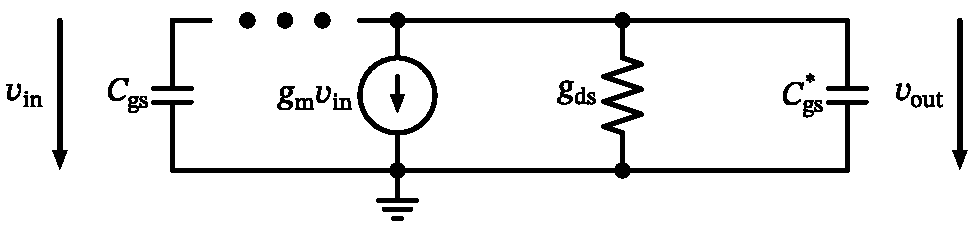
\includegraphics{index_files/mediabag/index_files/figure-pdf/fig-mosfet-diode-openloop-output-1.pdf}

}

\caption{\label{fig-mosfet-diode-openloop}The MOSFET diode small-signal
circuit for open-loop analysis.}

\end{figure}%

\textsubscript{Source:
\href{https://iic-jku.github.io/analog-circuit-design/index.qmd.html}{Article
Notebook}}

By inspecting Figure~\ref{fig-mosfet-diode-openloop} we see that \[
v_\mathrm{out} = - g_\mathrm{m}v_\mathrm{in} \frac{1}{g_\mathrm{ds}+ s C_\mathrm{gs}}.
\]

The open-loop gain \(H_\mathrm{ol}(s)\) is thus
\begin{equation}\phantomsection\label{eq-mosfet-diode-openloop-gain}{
H_\mathrm{ol}(s) = \frac{v_\mathrm{out}}{v_\mathrm{in}} = -\frac{g_\mathrm{m}}{g_\mathrm{ds}+ s C_\mathrm{gs}}.
}\end{equation}

Inspecting Equation~\ref{eq-mosfet-diode-openloop-gain} we realize that

\begin{enumerate}
\def\labelenumi{\arabic{enumi}.}
\tightlist
\item
  the dc gain \(g_\mathrm{m}/ g_\mathrm{ds}\) is the self-gain of the
  MOSFET, so
  \(20 \log(0.2 \cdot 10^{-3} / 9.6 \cdot 10 ^{-6}) = 26.4\,\text{dB}\),
  and
\item
  there is a pole at
  \(\omega_\mathrm{p} = -g_\mathrm{ds}/ C_\mathrm{gs}\), which is at
  \(9.6 \cdot 10 ^{-6} / (2 \pi \cdot 1.4 \cdot 10^{-15}) = 1.1\,\text{GHz}\).
\end{enumerate}

With this single pole location in \(H_\mathrm{ol}(s)\) this loop is
perfectly stable at under all conditions.

The question is now how to simulate this open-loop gain, and how to
break the loop open in simulation? In general there are various methods,
as we can use artificially large (ideal) inductors and capacitors to
break loops open and still establish the correct dc operating points for
the ac loop analysis. However, mimicking the correct loading can be an
issue, and requires a lot of careful consideration.

There is an alternative method which breaks the loop open only by adding
an ac voltage source in series (thus keeps the dc operating point
intact), or injects current using a current source. Based on both
measurements the open-loop gain can be calculated. This is called
\textbf{Middlebrook's method} (Middlebrook 1975) which is based on
double injection, and we will use it for our loop simulations. This
method is detailed in Section~\ref{sec-middlebrook-method}.

We now want to simulate the open-loop transfer function
\(H_\mathrm{ol}(s)\) by using Middlebrook's method and confirm our
analysis above.

\begin{tcolorbox}[enhanced jigsaw, colback=white, bottomtitle=1mm, titlerule=0mm, toprule=.15mm, coltitle=black, title=\textcolor{quarto-callout-tip-color}{\faLightbulb}\hspace{0.5em}{Exercise: MOSFET Diode Loop Analysis}, opacityback=0, leftrule=.75mm, opacitybacktitle=0.6, left=2mm, toptitle=1mm, arc=.35mm, colframe=quarto-callout-tip-color-frame, breakable, colbacktitle=quarto-callout-tip-color!10!white, rightrule=.15mm, bottomrule=.15mm]

Please build a simulation testbench in Xschem to simulate the open-loop
transfer function of the MOSFET diode. Confirm the dc gain and pole
location as given by Equation~\ref{eq-mosfet-diode-openloop-gain}.

If you are getting stuck you can look at this Xschem
\href{./xschem/mosfet_diode_loopgain.sch}{testbench}, shown in
Figure~\ref{fig-mosfet-diode-loopgain-tb}.

\begin{figure}[H]

\centering{

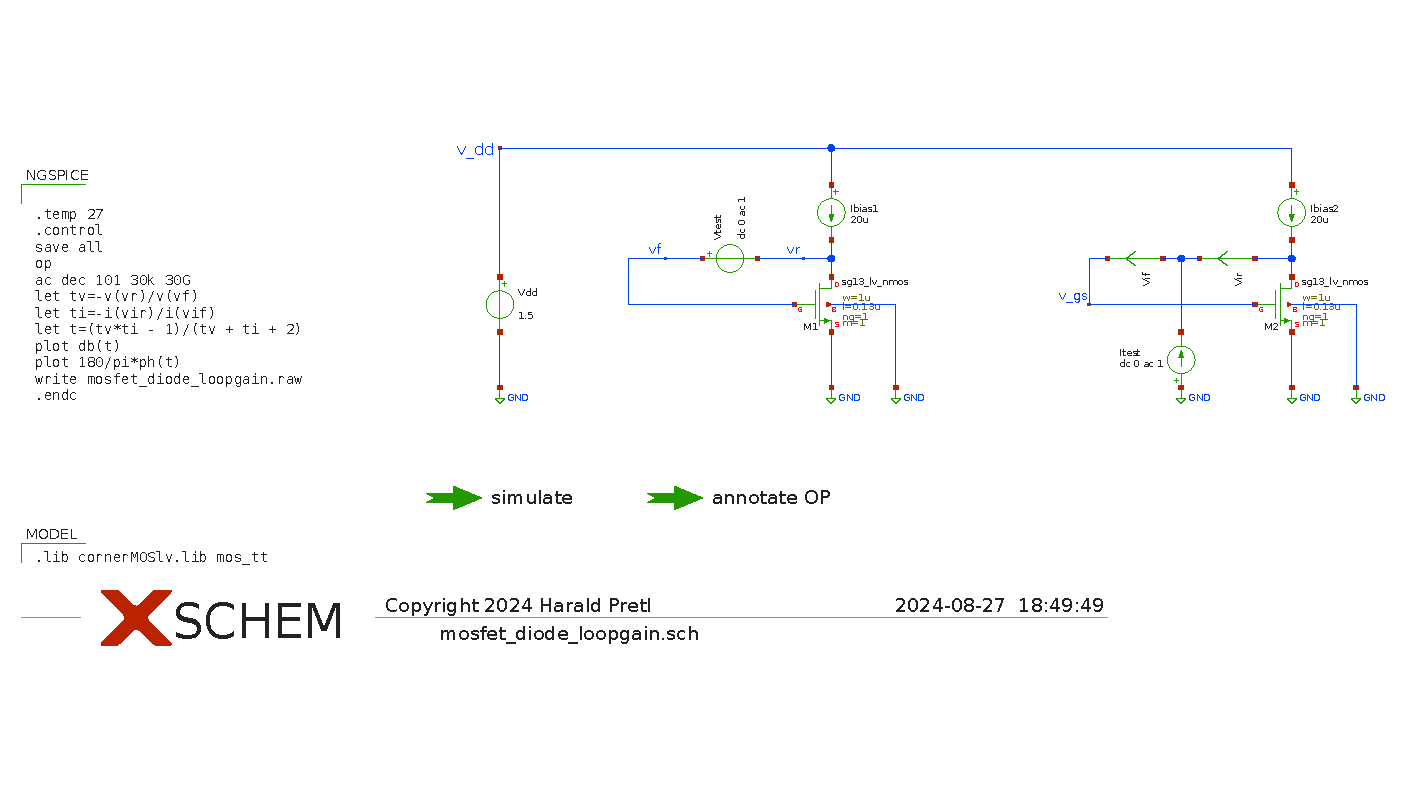
\includegraphics{index_files/mediabag/xschem/mosfet_diode_loopgain.pdf}

}

\caption{\label{fig-mosfet-diode-loopgain-tb}Testbench for MOSFET diode
stability analysis.}

\end{figure}%

\end{tcolorbox}

From simulation we see that the open-loop gain is \(24.9\,\text{dB}\) at
low frequencies, which matches quite well our prediction of
\(26.4\,\text{dB}\). In the Bode plot we see a low-pass with a
\(-3\,\text{dB}\) corner frequency of \(1.4\,\text{GHz}\), which again
is fairly close to our prediction of \(1.1\,\text{GHz}\).

\subsection{MOSFET Diode Noise
Calculation}\label{mosfet-diode-noise-calculation}

As a final exercise on the MOSFET diode circuit we want to calculate the
output noise when we consider \(V_\mathrm{GS}\) the output reference
voltage which is created when passing a bias current through the MOSFET
diode. The bias current we will assume noiseless.

We will use the small-signal circuit shown in
Figure~\ref{fig-mosfet-diode-small-signal-w-noise}.

\textsubscript{Source:
\href{https://iic-jku.github.io/analog-circuit-design/index.qmd.html}{Article
Notebook}}

\begin{figure}[H]

\centering{

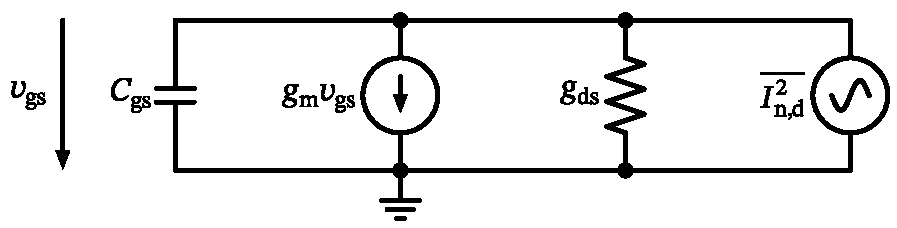
\includegraphics{index_files/mediabag/index_files/figure-pdf/fig-mosfet-diode-small-signal-w-noise-output-1.pdf}

}

\caption{\label{fig-mosfet-diode-small-signal-w-noise}The MOSFET diode
small-signal model with drain noise source.}

\end{figure}%

\textsubscript{Source:
\href{https://iic-jku.github.io/analog-circuit-design/index.qmd.html}{Article
Notebook}}

As we have already calculated the small-signal diode impedance in
Equation~\ref{eq-mosfet-diode-impedance} we will use this result, and
just note that the drain current noise of the MOSFET flows through this
impedance. The noise voltage at \(v_\mathrm{gs}\) is thus given as \[
\overline{V_\mathrm{n}^2} = Z_\mathrm{diode}^2 \overline{I_\mathrm{n,d}^2}.
\]

The drain current noise of the MOSFET is given as (introduced in
Section~\ref{sec-mosfet-smallsignal-model}) \[
\overline{I_\mathrm{n,d}^2} = 4 k T \gamma g_\mathrm{m}.
\]

For low frequencies (ignoring \(g_\mathrm{ds}\) and \(C_\mathrm{gs}\))
we get \[
\overline{V_\mathrm{n}^2} = Z_\mathrm{diode}^2 \overline{I_\mathrm{n,d}^2} = \frac{1}{g_\mathrm{m}^2} 4 k T \gamma g_\mathrm{m}= \frac{4 k T \gamma}{g_\mathrm{m}}
\] which is the thermal noise of a resistor of value
\(1 / g_\mathrm{m}\) enhanced by the factor \(\gamma\).

We now calculate the full equation, and after a bit of algebra arrive at
\begin{equation}\phantomsection\label{eq-mosfet-diode-noise-psd}{
\overline{V_\mathrm{n}^2}(f) = \frac{4 k T \gamma g_\mathrm{m}}{(g_\mathrm{m}+ g_\mathrm{ds})^2 + (2 \pi f C_\mathrm{gs})^2}.
}\end{equation}

If we are interested in the PSD of the noise then
Equation~\ref{eq-mosfet-diode-noise-psd} gives us the result. If we are
interested in the rms value (the total noise) we need to integrate this
equation, using the following identity:

\begin{tcolorbox}[enhanced jigsaw, colback=white, bottomtitle=1mm, titlerule=0mm, toprule=.15mm, coltitle=black, title=\textcolor{quarto-callout-note-color}{\faInfo}\hspace{0.5em}{Useful Integral for Noise Calculations}, opacityback=0, leftrule=.75mm, opacitybacktitle=0.6, left=2mm, toptitle=1mm, arc=.35mm, colframe=quarto-callout-note-color-frame, breakable, colbacktitle=quarto-callout-note-color!10!white, rightrule=.15mm, bottomrule=.15mm]

\begin{equation}\phantomsection\label{eq-integral-identity}{
\int_0^\infty {\frac{a}{b^2 + c^2 f^2} df} = \frac{\pi}{2} \frac{a}{b \cdot c}
}\end{equation}

\end{tcolorbox}

Using the integral help in Equation~\ref{eq-integral-identity}, we can
easily transform Equation~\ref{eq-mosfet-diode-noise-psd} to
\begin{equation}\phantomsection\label{eq-mosfet-diode-noise-rms}{
V_\mathrm{n,rms}^2 = \int_0^\infty \overline{V_\mathrm{n}^2}(f) df = \frac{k T \gamma g_\mathrm{m}}{(g_\mathrm{m}+ g_\mathrm{ds}) C_\mathrm{gs}}.
}\end{equation}

The form of Equation~\ref{eq-mosfet-diode-noise-rms} is the exact
solution, but we gain additional insight if we assume that
\(g_\mathrm{m}+ g_\mathrm{ds}\approx g_\mathrm{m}\) and then
\begin{equation}\phantomsection\label{eq-mosfet-diode-noise-rms-simplified}{
V_\mathrm{n,rms}^2 = \frac{k T \gamma}{C_\mathrm{gs}}.
}\end{equation}

Inspecting Equation~\ref{eq-mosfet-diode-noise-rms-simplified} we see
our familiar \(kT/C\) noise enhanced by the factor \(\gamma\)!
Calculating this value for our MOSFET diode we get
\(\sqrt{V_\mathrm{n,rms}^2} = \sqrt{1.38 \cdot 10^{-23} \cdot 300 \cdot 0.84 / 1.4 \cdot 10^{-15}} = 1.58\,\text{mV}\),
which is a sizeable value! We run circuits in this technology at
\(V_\mathrm{DD}= 1.5\,\mathrm{V}\), which leaves us with a signal swing
of ca. \(1.1\,\mathrm{V_{pp}}\), resulting in a dynamic range in this
case of \(20 \log (1.58 \cdot 10^{-3} / 0.39) \approx -48\,\text{dB}\).

\begin{tcolorbox}[enhanced jigsaw, colback=white, bottomtitle=1mm, titlerule=0mm, toprule=.15mm, coltitle=black, title=\textcolor{quarto-callout-important-color}{\faExclamation}\hspace{0.5em}{Large Bandwidth and Noise}, opacityback=0, leftrule=.75mm, opacitybacktitle=0.6, left=2mm, toptitle=1mm, arc=.35mm, colframe=quarto-callout-important-color-frame, breakable, colbacktitle=quarto-callout-important-color!10!white, rightrule=.15mm, bottomrule=.15mm]

Large BW circuits can integrate noise over a wide bandwidth resulting in
considerable rms noise.

\end{tcolorbox}

\begin{tcolorbox}[enhanced jigsaw, colback=white, bottomtitle=1mm, titlerule=0mm, toprule=.15mm, coltitle=black, title=\textcolor{quarto-callout-tip-color}{\faLightbulb}\hspace{0.5em}{Exercise: MOSFET Diode Noise}, opacityback=0, leftrule=.75mm, opacitybacktitle=0.6, left=2mm, toptitle=1mm, arc=.35mm, colframe=quarto-callout-tip-color-frame, breakable, colbacktitle=quarto-callout-tip-color!10!white, rightrule=.15mm, bottomrule=.15mm]

Please build a simulation testbench in Xschem to simulate the noise
performance of the MOSFET diode, and confirm the rms noise value that we
just calculated. Look at the rms value and the PSD of the noise, and
play around with the integration limits. What is the effect? Can you see
the flicker noise in the PSD? How much is its contribution to the rms
noise?

If you are getting stuck you can look at this Xschem
\href{./xschem/mosfet_diode_noise.sch}{testbench}, shown in
Figure~\ref{fig-mosfet-diode-noise-tb}.

\begin{figure}[H]

\centering{

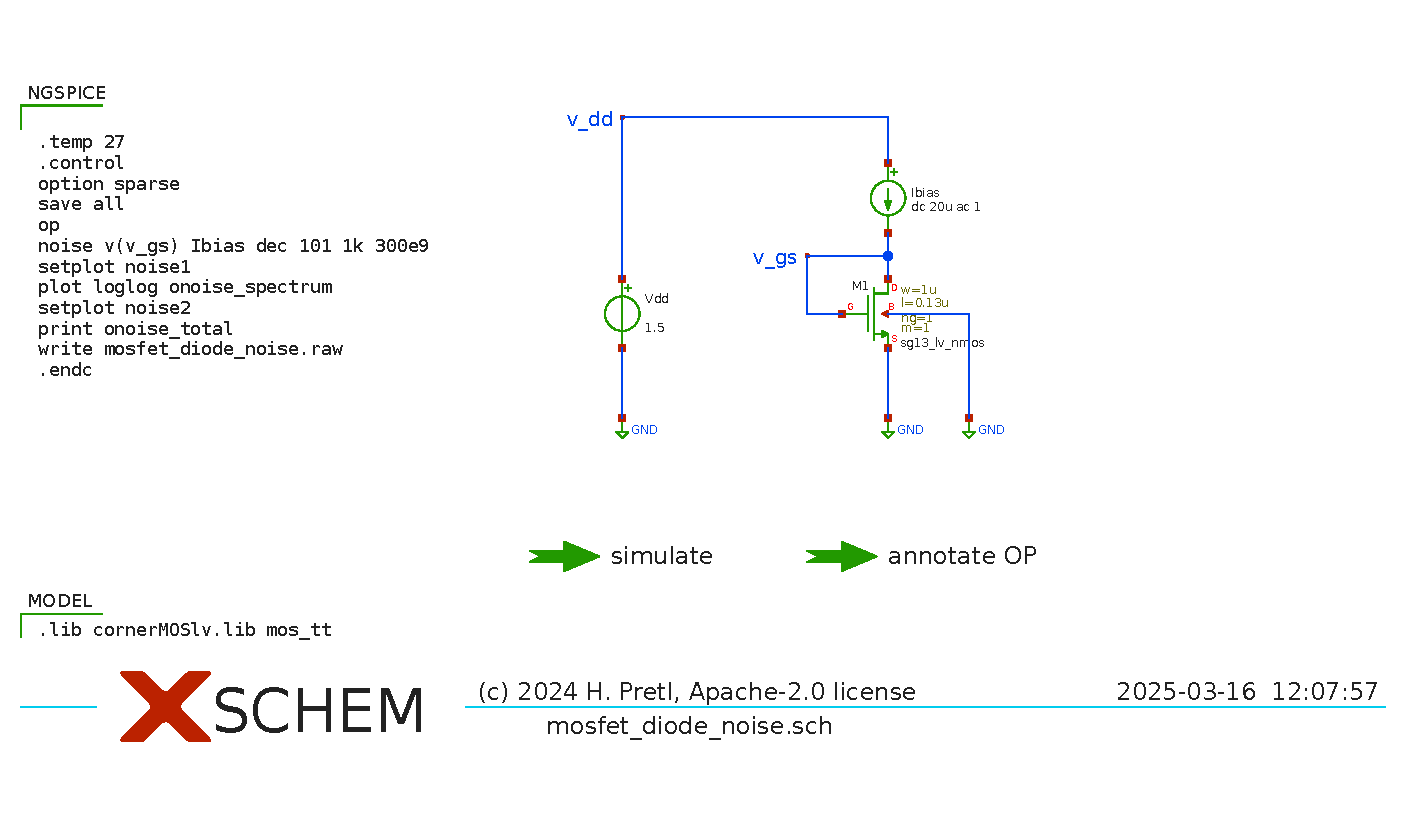
\includegraphics{index_files/mediabag/xschem/mosfet_diode_noise.pdf}

}

\caption{\label{fig-mosfet-diode-noise-tb}Testbench for MOSFET diode
noise analysis.}

\end{figure}%

\end{tcolorbox}

\subsection{Conclusion}\label{conclusion-1}

In this section we investigated the simple MOSFET-diode circuit. We
learned important skills like how to derive a small-signal model, how to
calculate important features like noise and open-loop gain for stability
analysis. We introduced Middlebrook's method to have a mechanism to open
up loops in simulation (and calculation) without disturbing operating
points for change loading conditions.

If you feel that you have not yet mastered these topics or are uncertain
in the operation of ngspice, please go back to the beginning of the
section and read through the theory and redo the exercises.

\section{Current Mirror}\label{sec-current-mirror}

In this section we will look into a fundamental building block which is
often used in integrated circuit design, the \textbf{current mirror}. A
diagram is shown in Figure~\ref{fig-current-mirror} with one MOSFET
diode converting the incoming bias current into a voltage, and two
output MOSFETs working as current sources, which are biased from the
diode. By properly selecting all \(W\) and \(L\) the input current can
be scaled, and multiple copies can be created at once. Shown in the
figure are two output currents, but any number of parallel branches can
be realized.

\textsubscript{Source:
\href{https://iic-jku.github.io/analog-circuit-design/index.qmd.html}{Article
Notebook}}

\begin{figure}[H]

\centering{

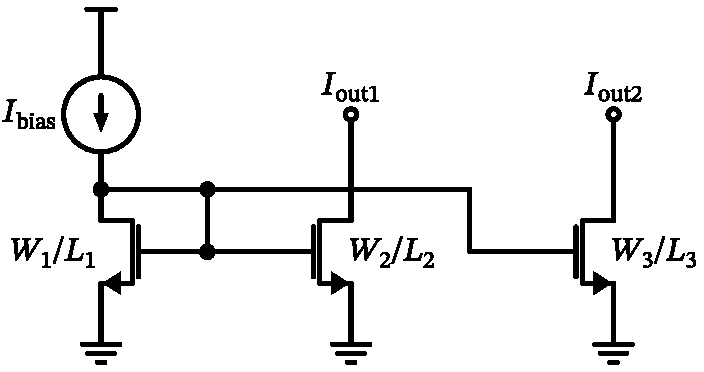
\includegraphics{index_files/mediabag/index_files/figure-pdf/fig-current-mirror-output-1.pdf}

}

\caption{\label{fig-current-mirror}A current mirror with two output
branches.}

\end{figure}%

\textsubscript{Source:
\href{https://iic-jku.github.io/analog-circuit-design/index.qmd.html}{Article
Notebook}}

The output current \(I_\mathrm{out1}\) is then given by \[
I_\mathrm{out1} = I_\mathrm{bias} \frac{W_2}{L_2} \frac{L_1}{W_1}
\] and the output current \(I_\mathrm{out2}\) is given by \[
I_\mathrm{out2} = I_\mathrm{bias} \frac{W_3}{L_3} \frac{L_1}{W_1}.
\]

For good matching in layout care has to be taken that the MOSFET widths
and lengths are constructed out of \textbf{unit elements} of identical
size, where an appropiate amount of these single units are then arranged
in series or parallel configuration to arrive at the target \(W\) and
\(L\).

As we know from earlier investigations of the MOSFET performance in
Section~\ref{sec-gmid-method} the drain current of a MOSFET is a
function of \(V_\mathrm{GS}\) and \(V_\mathrm{DS}\). As long as the
MOSFET stays in saturation (i.e., \(V_\mathrm{DS}> V_\mathrm{ds,dsat}\))
the drain current is just a mild function of \(V_\mathrm{DS}\)
(essentially the effect of \(g_\mathrm{ds}\), which is the output
conductance of the MOSFET). A fundamental flaw of the basic current
mirror shown in Figure~\ref{fig-current-mirror} is the mismatch of the
\(V_\mathrm{DS}\) of the MOSFET. The input-side diode has
\(V_\mathrm{GS}= V_\mathrm{DS}\), whereas the output current sources
have a \(V_\mathrm{DS}\) depending on the connected circuitry. Improved
current mirrors exist (basically fixing this flaw), still, when just a
simple current mirror is required this structure is used for its
simplicity.

\begin{tcolorbox}[enhanced jigsaw, colback=white, bottomtitle=1mm, titlerule=0mm, toprule=.15mm, coltitle=black, title=\textcolor{quarto-callout-tip-color}{\faLightbulb}\hspace{0.5em}{Exercise: Current Mirror}, opacityback=0, leftrule=.75mm, opacitybacktitle=0.6, left=2mm, toptitle=1mm, arc=.35mm, colframe=quarto-callout-tip-color-frame, breakable, colbacktitle=quarto-callout-tip-color!10!white, rightrule=.15mm, bottomrule=.15mm]

Please construct a current mirror based on the MOSFET-diode which we
sized in Section~\ref{sec-mosfet-diode}. The input current
\(I_\mathrm{bias} = 20\,\mu\text{A}\), and we want three output currents
of size \(10\,\mu\text{A}\), \(20\,\mu\text{A}\), and
\(40\,\mu\text{A}\).

Sweep the output voltage of all three current branches and see over
which voltage range an acceptable current is created. For which output
voltage range is the current departing from its ideal value, and why?

You see that the slope of the output current is quite bad, as
\(g_\mathrm{ds}\) is too large. We can improve this by changing the
length to \(L = 5\,\mu\text{m}\) (for motivation, please look at the
graphs in Section~\ref{sec-gmid-method}). In addition, for a current
mirror we are not interested in a high \(g_\mathrm{m}/I_\mathrm{D}\)
value, so we can use \(g_\mathrm{m}/I_\mathrm{D}= 5\) in this case.
Please size the current mirror MOSFETs accordinly (please round the
\(W\) to half micron, to keep sizes a bit more practical). Compare this
result to the previous one, what changed?

In case you get stuck, here are Xschem schematics for the
\href{./xschem/current_mirror.sch}{original} and the
\href{./xschem/current_mirror_improved.sch}{improved} current mirrors.

\end{tcolorbox}

\section{Differential Pair}\label{sec-diff-pair}

Like the current mirror in Section~\ref{sec-current-mirror} the
\textbf{differential pair} is an ubiquitous building block often used in
integrated circuit design. The fundamental structure is given in
Figure~\ref{fig-differential-pair}.

\textsubscript{Source:
\href{https://iic-jku.github.io/analog-circuit-design/index.qmd.html}{Article
Notebook}}

\begin{figure}[H]

\centering{

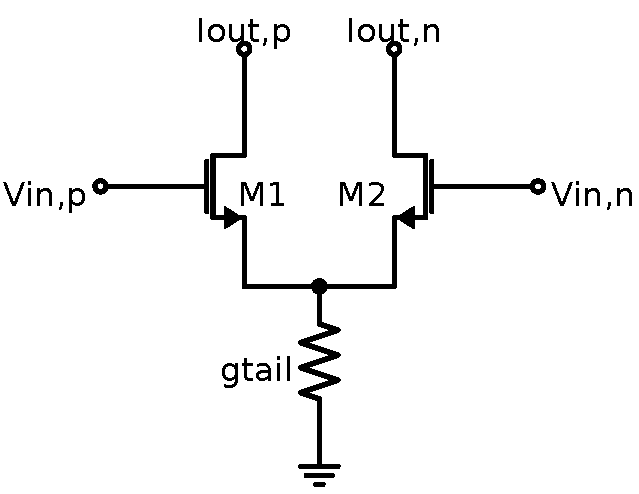
\includegraphics{index_files/mediabag/index_files/figure-pdf/fig-differential-pair-output-1.pdf}

}

\caption{\label{fig-differential-pair}A differential pair.}

\end{figure}%

\textsubscript{Source:
\href{https://iic-jku.github.io/analog-circuit-design/index.qmd.html}{Article
Notebook}}

In order to understand its operation it is instructive to separate the
input condition into (1) a purely differential voltage, and (2) into a
common-mode voltage, and see what the impact on the output currents is.

\subsection{Differential Operation of the
Diffpair}\label{differential-operation-of-the-diffpair}

For a differential mode of operation we assume that the input common
mode voltage is constant,
i.e.~\(V_\mathrm{in,p} + V_\mathrm{in,n} = V_\mathrm{CM}\). A
differential input voltage \(v_\mathrm{in}\) then results in \[
V_\mathrm{in,p} = V_\mathrm{CM} + \frac{v_\mathrm{in}}{2}
\] and \[
V_\mathrm{in,n} = V_\mathrm{CM} - \frac{v_\mathrm{in}}{2}.
\]

For a small-signal differential drive the potential at the tail point
stays constant and we can treat it as a virtual ground. The output
current on each side is then given by (neglecting \(g_\mathrm{ds}\) and
\(g_\mathrm{mb}\) of \(M_1\) and \(M_2\)) \[
i_\mathrm{out,p} = g_\mathrm{m1} \left( \frac{v_\mathrm{in}}{2} \right)
\] and \[
i_\mathrm{out,n} = g_\mathrm{m2} \left( -\frac{v_\mathrm{in}}{2} \right).
\]

Usually we assume symmetry in the differential pair, so
\(g_\mathrm{m1} = g_\mathrm{m2} = g_\mathrm{m}\). The differential
output current \(i_\mathrm{out}\) is then given by
\begin{equation}\phantomsection\label{eq-differential-pair-dm}{
i_\mathrm{out} = i_\mathrm{out,p} - i_\mathrm{out,n} = g_\mathrm{m}v_\mathrm{in}
}\end{equation}

We see in Equation~\ref{eq-differential-pair-dm} that the differential
output current is simply the differential input voltage multiplied by
the \(g_\mathrm{m}\) of the individual transistor. We also note that the
bottom conductance \(g_\mathrm{tail}\) plays no role for the
small-signal differential operation.

\subsection{Common-Mode Operation of the
Diffpair}\label{common-mode-operation-of-the-diffpair}

Usually, the source conductance \(g_\mathrm{tail}\) is realized by a
current source and ideally should be \(g_\mathrm{tail} = 0\). If this is
the case, then the output currents are not a function of the common-mode
input voltage, and (\(I_\mathrm{tail}\) is set by the tail current
source) \[
I_\mathrm{out,p} = I_\mathrm{out,n} = \frac{I_\mathrm{tail}}{2}.
\]

However, if we assume a realistic tail current source then
\(g_\mathrm{tail} > 0\). For analysis we can simply look at a half
circuit since everything is symmetric. In order to simplify the analysis
a bit we remove all capacitors from the MOSFET small-signal model and
set \(g_\mathrm{ds}= g_\mathrm{mb}= 0\). We arrive then at the
small-signal equivalent circuit shown in
Figure~\ref{fig-differential-pair-cm} (note that we set
\(v_\mathrm{in,p} = v_\mathrm{in,n} = v_\mathrm{in}\) and
\(i_\mathrm{out,p} = i_\mathrm{out,n} = i_\mathrm{out}\) under symmetry
considerations).

\textsubscript{Source:
\href{https://iic-jku.github.io/analog-circuit-design/index.qmd.html}{Article
Notebook}}

\begin{figure}[H]

\centering{

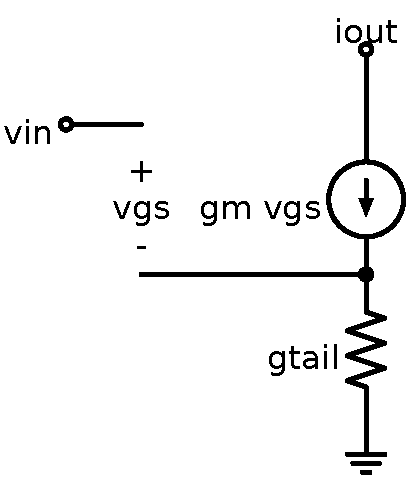
\includegraphics{index_files/mediabag/index_files/figure-pdf/fig-differential-pair-cm-output-1.pdf}

}

\caption{\label{fig-differential-pair-cm}Small-signal model of the
differential pair half-circuit in common-mode operation.}

\end{figure}%

\textsubscript{Source:
\href{https://iic-jku.github.io/analog-circuit-design/index.qmd.html}{Article
Notebook}}

Formulating KVL for the input-side loop we get \[
v_\mathrm{in} = v_\mathrm{gs}+ \frac{i_\mathrm{ds}}{g_\mathrm{tail}}.
\]

With \(i_\mathrm{out} = i_\mathrm{ds}= g_\mathrm{m}v_\mathrm{gs}\) we
arrive at
\begin{equation}\phantomsection\label{eq-differential-pair-cm}{
i_\mathrm{out} = \frac{g_\mathrm{m}g_\mathrm{tail}}{g_\mathrm{m}+ g_\mathrm{tail}} v_\mathrm{in}
}\end{equation}

Interpreting Equation~\ref{eq-differential-pair-cm} we can distinguish
the following extreme cases:

\begin{enumerate}
\def\labelenumi{\arabic{enumi}.}
\tightlist
\item
  If \(g_\mathrm{tail} = 0\) (ideal tail current source) then
  \(i_\mathrm{out} = 0\), the common-mode voltage variation from the
  input is suppressed and does not show up at the common-mode output
  current (which is constant due to the ideal tail current source). This
  is usually the case that we want to achieve.
\item
  If \(g_\mathrm{tail} = \infty\) then
  \(i_\mathrm{out} = g_\mathrm{m}v_\mathrm{in}\), which means the output
  current is a function of the MOSFET \(g_\mathrm{m}\). If everything is
  perfectly matched, then the differential output current is zero, but
  the common-mode output current changes according to the common-mode
  input voltage. In special cases this can be a wanted behaviour, this
  configuration is called a ``pseudo-differential pair.''
\end{enumerate}

\section{A Basic 5-Transistor OTA}\label{sec-basic-ota}

Suited with the knowledge of basic transitor operation
(Section~\ref{sec-first-steps} and Section~\ref{sec-gmid-method}) and
the working knowledge of the current mirror
(Section~\ref{sec-mosfet-diode} and Section~\ref{sec-current-mirror}) as
well as the differential pair (Section~\ref{sec-diff-pair}) we can now
start to design our first real circuit. A fundamental (simple) circuit
that is often used for basic tasks is the 5-transistor operational
transconductance amplifier (OTA). A circuit diagram of this 5T-OTA is
shown in Figure~\ref{fig-basic-ota}.

\textsubscript{Source:
\href{https://iic-jku.github.io/analog-circuit-design/index.qmd.html}{Article
Notebook}}

\begin{figure}[H]

\centering{

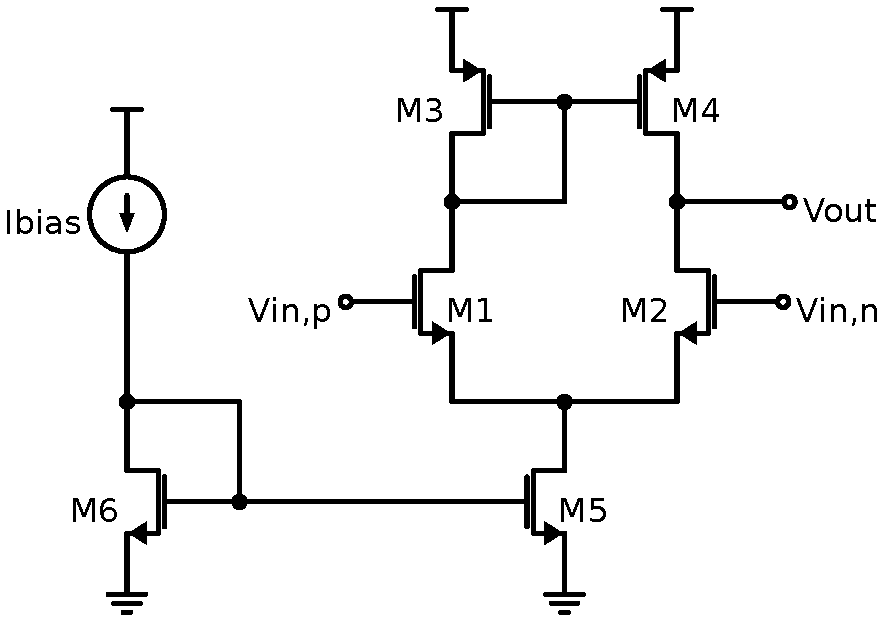
\includegraphics{index_files/mediabag/index_files/figure-pdf/fig-basic-ota-output-1.pdf}

}

\caption{\label{fig-basic-ota}The 5-transistor OTA.}

\end{figure}%

\textsubscript{Source:
\href{https://iic-jku.github.io/analog-circuit-design/index.qmd.html}{Article
Notebook}}

The operation is as follows: \(M_{1,2}\) form a differential pair which
is biased by the current source \(M_5\). \(M_{5,6}\) form a current
mirror, thus the input bias current \(I_\mathrm{bias}\) sets the bias
current in the OTA. The differential pair \(M_{1,2}\) is loaded by the
current mirror \(M_{3,4}\) which mirrors the output current of \(M_1\)
to the right side. Here, the currents from \(M_4\) and \(M_2\) are
summed, and together with the conductance effective at the output node a
voltage builds up.

We note that \(M_{1,2}\) and \(M_{3,4}\) need to be symmetric, thus will
have the same \(W\) and \(L\) dimensioning. \(M_{5,6}\) we scale
accordingly to set the correct bias current in the OTA.

As this is an OTA the output is a current; if the load impedance is high
(i.e., purely capacitive, which is often the case in integrated circuits
when driving MOSFET inputs) then the voltage gain of the OTA can be high
(of course, in this simple OTA it is limited). With a high-impedance
loading this OTA can provide a voltage output, and this is actually how
OTAs are mostly operated.

\subsection{Voltage Buffer with OTA}\label{voltage-buffer-with-ota}

In order to design an OTA we need an application, and from this we need
to derive the circuit specifications. We want to use this OTA to realize
a voltage buffer which lighly loads a voltage source and can drive a
large capacitive load. Such a configuration is often used to, e.g.,
buffer a reference voltage that is needed (and thus loaded) by another
circuit. The block diagram of this configuration is shown in
Figure~\ref{fig-voltage-buffer-ota}.

\textsubscript{Source:
\href{https://iic-jku.github.io/analog-circuit-design/index.qmd.html}{Article
Notebook}}

\begin{figure}[H]

\centering{

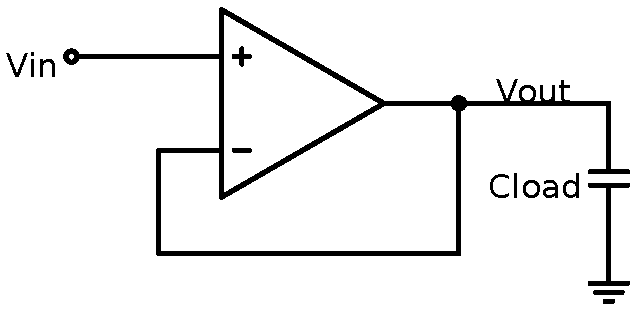
\includegraphics{index_files/mediabag/index_files/figure-pdf/fig-voltage-buffer-ota-output-1.pdf}

}

\caption{\label{fig-voltage-buffer-ota}A voltage buffer (based on OTA)
driving a capacitive load.}

\end{figure}%

\textsubscript{Source:
\href{https://iic-jku.github.io/analog-circuit-design/index.qmd.html}{Article
Notebook}}

If the voltage gain of the OTA is Figure~\ref{fig-voltage-buffer-ota} is
high, then \(V_\mathrm{out} \approx V_\mathrm{in}\). We now want to
design an OTA for this application for the following spefication values
(see Table~\ref{tbl-voltage-buffer-spec}). These values are rather
typical of what could be expected for such a buffer design.

\begin{longtable}[]{@{}
  >{\raggedright\arraybackslash}p{(\columnwidth - 4\tabcolsep) * \real{0.5588}}
  >{\centering\arraybackslash}p{(\columnwidth - 4\tabcolsep) * \real{0.3529}}
  >{\centering\arraybackslash}p{(\columnwidth - 4\tabcolsep) * \real{0.0882}}@{}}
\caption{Voltage buffer
specification}\label{tbl-voltage-buffer-spec}\tabularnewline
\toprule\noalign{}
\begin{minipage}[b]{\linewidth}\raggedright
Specification
\end{minipage} & \begin{minipage}[b]{\linewidth}\centering
Value
\end{minipage} & \begin{minipage}[b]{\linewidth}\centering
Unit
\end{minipage} \\
\midrule\noalign{}
\endfirsthead
\toprule\noalign{}
\begin{minipage}[b]{\linewidth}\raggedright
Specification
\end{minipage} & \begin{minipage}[b]{\linewidth}\centering
Value
\end{minipage} & \begin{minipage}[b]{\linewidth}\centering
Unit
\end{minipage} \\
\midrule\noalign{}
\endhead
\bottomrule\noalign{}
\endlastfoot
Supply voltage & \(1.45 < \underline{1.5} < 1.55\) & V \\
Temperature range (industrial) & \(-40 < \underline{27} < 125\) &
degC \\
Load capacitance \(C_\mathrm{load}\) & \(50\) & fF \\
Input voltage range (for buffering 2/3 bandgap voltage) &
\(0.7 < \underline{0.8} < 0.9\) & V \\
Signal bandwidth (3dB) & \(>10\) & MHz \\
Output voltage error & \(<3\) & \% \\
Total output noise (rms) & \(<1\) & mV\textsubscript{rms} \\
Supply current (as low as possible) & \(<10\) & µA \\
Stability & stable for rated \(C_\mathrm{load}\) & \\
Turn-on time (settled to with 1\%) & \(<10\) & µs \\
Externally provided bias current (nominal) & \(20\) & µA \\
\end{longtable}

\subsection{Large-Signal Analysis of the
OTA}\label{sec-basic-ota-large-signal}

The first step when receiving a design task is to look at the
specifications, and see whether they make sense. Detailed performance of
the design will be the result of the circuit simulation, but before we
step into sizing we need to do a few simple calculations to (a) allows
to do back-of-the-envelope gauging if the specification makes sense, and
(b) the derived analytical equations will serve as guide for the sizing
procedure.

\begin{itemize}
\tightlist
\item
  In terms of large-signal operation, we will now check whether the
  input and output voltage range, as well as the settling time can be
  roughly met.
\item
  When the input is at its maximum of \(0.9\,\text{V}\), we see that we
  need to keep \(M_1\) in saturation. We can calculate that
  \(V_\mathrm{DS1} = V_\mathrm{DD}- |V_\mathrm{GS3}| + V_\mathrm{GS1} - V_\mathrm{in} = 1.45 - 0.6 + 0.6 - 0.9 = 0.55\,\text{V}\),
  which leaves enough margin.
\item
  When the input is at its minimum of \(0.7\,\text{V}\), we see that the
  \(V_\mathrm{DS5}\) of \(M_5\) is calculated as
  \(V_\mathrm{DS5} = V_\mathrm{in} - V_\mathrm{GS1} = 0.7 - 0.6 = 0.1\,\text{V}\),
  so this leaves little margin, but likely \(V_\mathrm{GS1}\) will be
  smaller, so it should work out.
\item
  For the output voltage, when the output voltage is on the high side,
  it leaves
  \(|V_\mathrm{DS4}| = V_\mathrm{DD}- V_\mathrm{out} = 1.45 - 0.9 = 0.55\,\text{V}\),
  which is enough margin.
\end{itemize}

In summary, we think that we can make an NMOS-input OTA like the one in
Figure~\ref{fig-basic-ota} work for the required supply and input- and
output voltages. If this would not work out, we need to look for further
options, like a PMOS-input OTA, or a NMOS/PMOS-input OTA.

Another large-signal specification item that we can quickly check is the
settling time. Under slewing conditions, the complete bias current in
the OTA is steered towards the output (try to understand why this is the
case), so when the output capacitor is fully discharged, and we assume
just a linear ramp due to constant-current charging of the output
capacitor, the settling time is \[
T_\mathrm{slew} \approx \frac{C_\mathrm{load} V_\mathrm{out}}{I_\mathrm{tail}} = \frac{50 \cdot 10^{-15} \cdot 1.3}{10 \cdot 10^{-6}} = 6.5\,\text{ns}
\] so this leaves plenty of margin for additional slow-signal settling
due to the limited bandwidth, as well as reducing the supply current.

The small-signal settling (assuming one pole at the bandwidth corner
frequency) leads to an approximate settling time (1\% error corresponds
to \(\approx 5 \tau\)) of \[
T_\mathrm{slew} \approx \frac{5}{2 \pi f_\mathrm{c}} = \frac{5}{2 \pi \cdot 1 \cdot 10^{-6}} = 0.8\,\mu\text{s}.
\] which also checks out.

\subsection{Small-Signal Analysis of the
OTA}\label{sec-basic-ota-small-signal}

In order to size the OTA components we need to derive how MOSFET
parameters define the performance. The important small-signal metrics
are

\begin{itemize}
\tightlist
\item
  dc gain \(A_0\)
\item
  gain-bandwidth product (GBW)
\item
  output noise
\end{itemize}

The specification for GBW is given in
Table~\ref{tbl-voltage-buffer-spec}, the dc gain we have to calculate
from the voltage accuracy specification. For a voltage follower in the
configuration shown in Figure~\ref{fig-voltage-buffer-ota} the voltage
gain is given by \[
\frac{V_\mathrm{out}}{V_\mathrm{in}} = \frac{A_0}{1 + A_0}.
\]

So in order to reach an output voltage accuracy of at least 3\% we need
a dc gain of \(A_0 > 30.2\,\text{dB}\). To allow for process and
temperature variation we need to add a bit of extra gain as margin.

\subsubsection{OTA Small-Signal Transfer
Function}\label{ota-small-signal-transfer-function}

In order to derive the governing equations for the OTA we will make a
few simplifications:

\begin{itemize}
\tightlist
\item
  We will set \(g_\mathrm{mb}= 0\) for all MOSFETs.
\item
  We will further set \(C_\mathrm{gd}= 0\) for all MOSFETs except for
  \(M_4\) where we expect a Miller effect on this capacitor, and we
  could add its effect by increasing the capacitance at the gate node of
  \(M_{3,4}\). Hoewever, as this does not create a dominant pole in this
  circuit, we consider this a minor effect (see
  Equation~\ref{eq-simple-ota-gain}).
\item
  We assume \(g_\mathrm{m}\gg g_\mathrm{ds}\), so we set
  \(g_\mathrm{ds1} = g_\mathrm{ds3} = 0\).
\item
  The drain capacitance of \(M_2\) and \(M_4\), as well as the gate
  capacitance of \(M_2\) we can add to the load capacitance
  \(C_\mathrm{load}\).
\end{itemize}

The resulting small-signal equivalent circuit is shown in
Figure~\ref{fig-basic-ota-small-signal}.

\begin{tcolorbox}[enhanced jigsaw, colback=white, bottomtitle=1mm, titlerule=0mm, toprule=.15mm, coltitle=black, title=\textcolor{quarto-callout-warning-color}{\faExclamationTriangle}\hspace{0.5em}{Refresh MOSFET Small-Signal Model}, opacityback=0, leftrule=.75mm, opacitybacktitle=0.6, left=2mm, toptitle=1mm, arc=.35mm, colframe=quarto-callout-warning-color-frame, breakable, colbacktitle=quarto-callout-warning-color!10!white, rightrule=.15mm, bottomrule=.15mm]

Please review the MOSFET small-signal equivalent model in
Figure~\ref{fig-mosfet-small-signal-model} at this point. For the PMOS
just flip the model upside-down.

\end{tcolorbox}

\textsubscript{Source:
\href{https://iic-jku.github.io/analog-circuit-design/index.qmd.html}{Article
Notebook}}

\begin{figure}[H]

\centering{

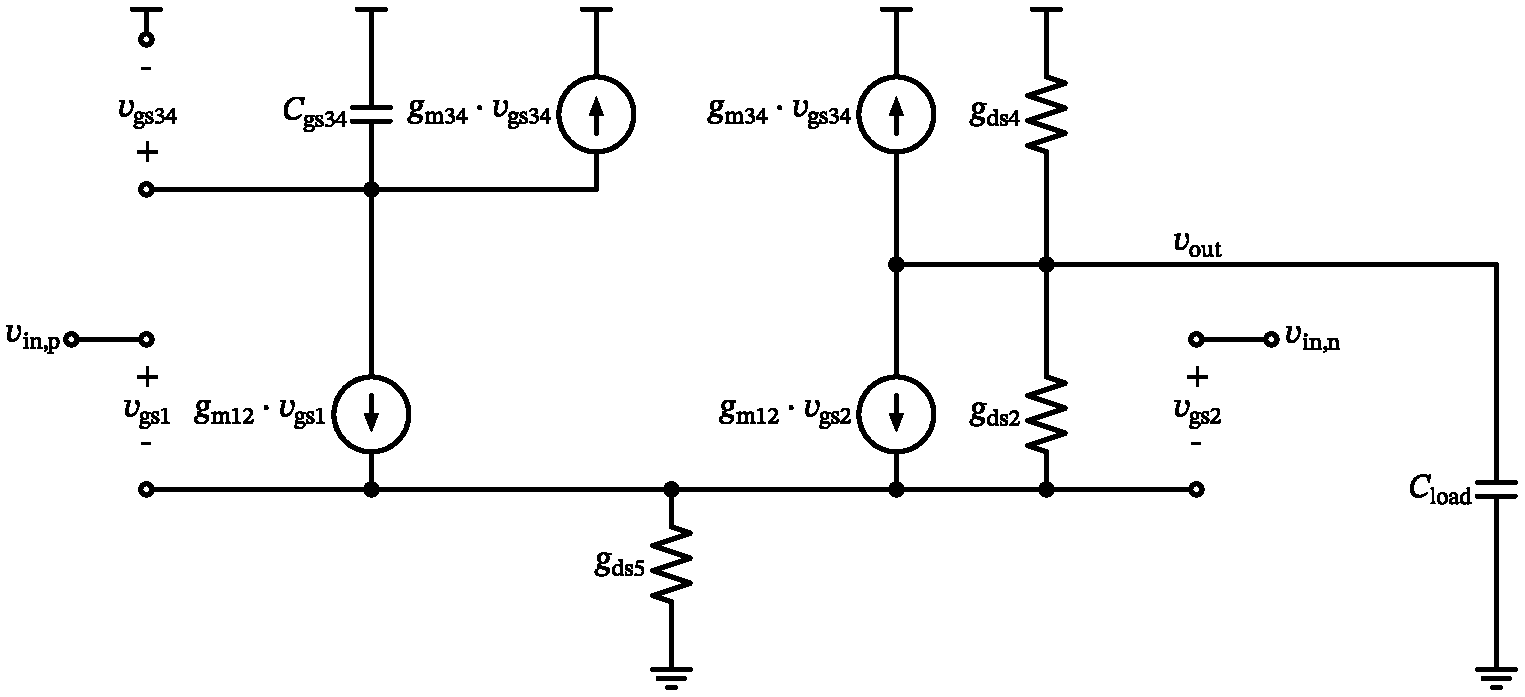
\includegraphics{index_files/mediabag/index_files/figure-pdf/fig-basic-ota-small-signal-output-1.pdf}

}

\caption{\label{fig-basic-ota-small-signal}5-transistor OTA small-signal
model.}

\end{figure}%

\textsubscript{Source:
\href{https://iic-jku.github.io/analog-circuit-design/index.qmd.html}{Article
Notebook}}

We can further simplify the output side by recognizing that the
impedance looking from the output down we have \(g_\mathrm{ds2}\) in
series with \(g_\mathrm{ds5} + g_\mathrm{m12}\) (since we treat \(M_1\)
as a common-gate stage when looking from the output, and since it is
loaded by a low impedance of \(g_\mathrm{m34}^{-1}\) we can approximate
the impedance looking into \(M_1\) with \(g_\mathrm{m12}^{-1}\)). With
the approximation that \(g_\mathrm{m}\gg g_\mathrm{ds}\) we can move
\(g_\mathrm{ds2} + g_\mathrm{ds4}\) in parallel to \(C_\mathrm{load}\).
Further, assuming a differential drive with a virtual ground at the
tailpoint we can remove \(g_\mathrm{ds5}\). The current source
\(g_\mathrm{m34} v_\mathrm{gs34}\) with replace with the equivalent
conductance \(g_\mathrm{m34}\). This results in the further simplified
equivalent circuit shown in
Figure~\ref{fig-basic-ota-small-signal-simplified}.

\textsubscript{Source:
\href{https://iic-jku.github.io/analog-circuit-design/index.qmd.html}{Article
Notebook}}

\begin{figure}[H]

\centering{

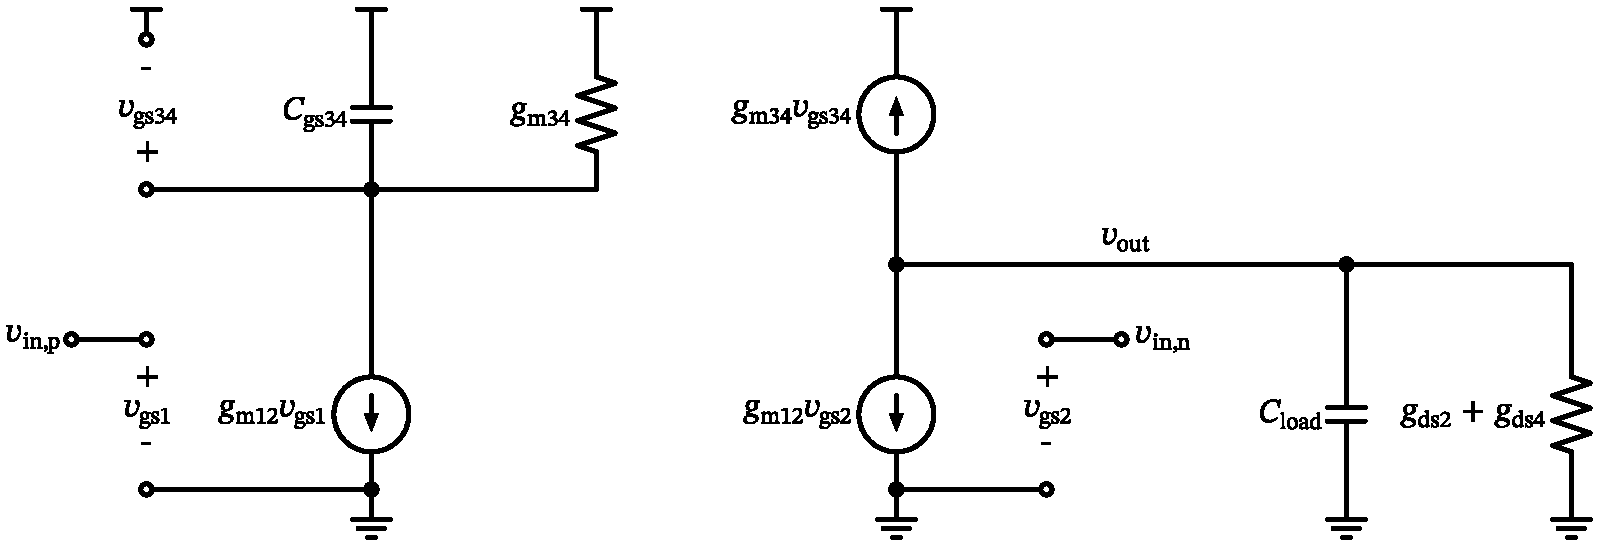
\includegraphics{index_files/mediabag/index_files/figure-pdf/fig-basic-ota-small-signal-simplified-output-1.pdf}

}

\caption{\label{fig-basic-ota-small-signal-simplified}5-transistor OTA
small-signal model with further simplifications.}

\end{figure}%

\textsubscript{Source:
\href{https://iic-jku.github.io/analog-circuit-design/index.qmd.html}{Article
Notebook}}

In the simplified circuit model in
Figure~\ref{fig-basic-ota-small-signal-simplified} we can see that we
have two poles in the circuit, one at the gate note of \(M_{3,4}\), and
one at the output. Realizing that \(v_\mathrm{in,p} = v_\mathrm{in}/2\)
and \(v_\mathrm{in,n} = - v_\mathrm{in}/2\) we can formulate KCL at the
output node to \begin{equation}\phantomsection\label{eq-simple-ota-eq1}{
-g_\mathrm{m34} V_\mathrm{gs34} - \left( -g_\mathrm{m12} \frac{V_\mathrm{in}}{2} \right) - V_\mathrm{out} (g_\mathrm{ds2} + g_\mathrm{ds4} + s C_\mathrm{load}) = 0.
}\end{equation} We further realize that
\begin{equation}\phantomsection\label{eq-simple-ota-eq2}{
V_\mathrm{gs34} = -g_\mathrm{m12} \frac{V_\mathrm{in}}{2} \frac{1}{g_\mathrm{m34} + s C_\mathrm{gs34}}.
 }\end{equation}

By combining Equation~\ref{eq-simple-ota-eq1} and
Equation~\ref{eq-simple-ota-eq2} and after a bit of algebraic
manipulation we arrive at
\begin{equation}\phantomsection\label{eq-simple-ota-gain}{
A(s) = \frac{V_\mathrm{out}}{V_\mathrm{in}} = \frac{g_\mathrm{m12}}{2} \frac{2 g_\mathrm{m34} + s C_\mathrm{gs34}}{(g_\mathrm{m34} + s C_\mathrm{gs34}) (g_\mathrm{ds2} + g_\mathrm{ds4} + s C_\mathrm{load})}.
}\end{equation}

When we now inspect Equation~\ref{eq-simple-ota-gain} we can see that
for low frequencies the gain is
\begin{equation}\phantomsection\label{eq-simple-ota-gain-dc}{
A(s \rightarrow 0) = A_0 = \frac{g_\mathrm{m12}}{g_\mathrm{ds2} + g_\mathrm{ds4}}
}\end{equation} which is plausible, and confirms the requirement of a
high impedance at the output node. For very large frequencies we get
\begin{equation}\phantomsection\label{eq-simple-ota-highf}{
A (s \rightarrow \infty) = \frac{g_\mathrm{m12}}{2 s C_\mathrm{load}}
}\end{equation} which is essentially the behaviour of an integrator, and
we can use Equation~\ref{eq-simple-ota-highf} to calculate the frequency
where the gain drops to \(1\): \[
f_\mathrm{ug} = \frac{g_\mathrm{m12}}{4 \pi C_\mathrm{load}}
\]

when looking at Equation~\ref{eq-simple-ota-gain} we see that we have a
dominant pole at \(s_\mathrm{p}\) and a pole-zero doublet with
\(s_\mathrm{pd}\)/\(s_\mathrm{zd}\): \[
s_\mathrm{p} = -\frac{g_\mathrm{ds2} + g_\mathrm{ds4}}{C_\mathrm{load}}
\] \[
s_\mathrm{pd} = -\frac{g_\mathrm{m34}}{C_\mathrm{gs34}}
\] \[
s_\mathrm{zd} = -\frac{2 g_\mathrm{m34}}{C_\mathrm{gs34}}
\]

\subsubsection{OTA Noise}\label{ota-noise}

For the noise analysis we ignore the pole-zero doublet due to
\(C_\mathrm{gs34}\) (we assume minor impact due to this) and just
consider the dominant pole. For the noise analysis at the output we set
the input signal to zero, and thus we arrive at the simplified
small-signal circuit shown in
Figure~\ref{fig-basic-ota-small-signal-noise}.

\textsubscript{Source:
\href{https://iic-jku.github.io/analog-circuit-design/index.qmd.html}{Article
Notebook}}

\begin{figure}[H]

\centering{

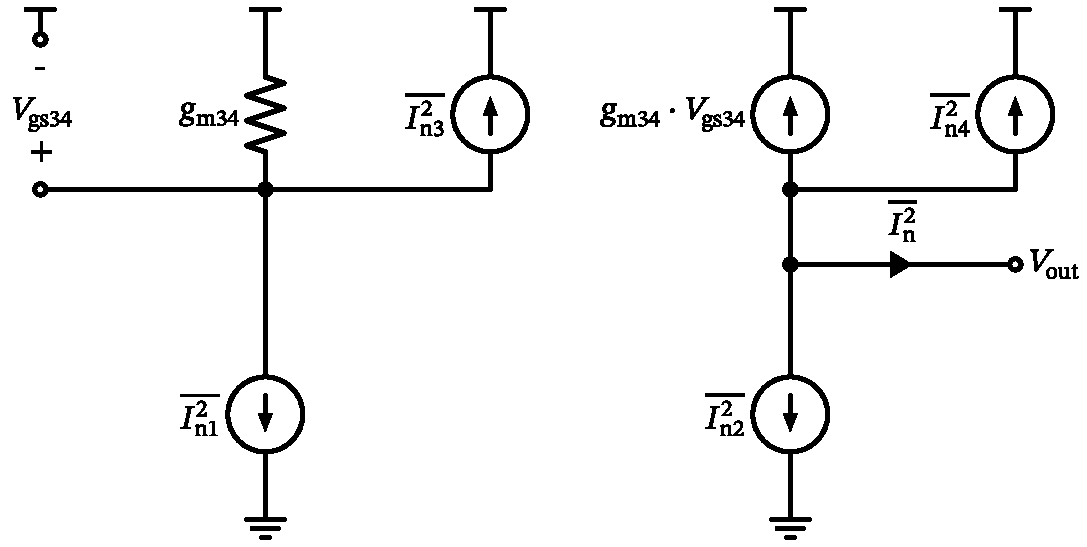
\includegraphics{index_files/mediabag/index_files/figure-pdf/fig-basic-ota-small-signal-noise-output-1.pdf}

}

\caption{\label{fig-basic-ota-small-signal-noise}5-transistor OTA
small-signal model for noise calculation.}

\end{figure}%

\textsubscript{Source:
\href{https://iic-jku.github.io/analog-circuit-design/index.qmd.html}{Article
Notebook}}

We see that \[
\overline{V_\mathrm{gs34}^2} = \frac{1}{g_\mathrm{m34}^2} \left( \overline{I_\mathrm{n1}^2} + \overline{I_\mathrm{n3}^2} \right).
\]

\begin{tcolorbox}[enhanced jigsaw, colback=white, bottomtitle=1mm, titlerule=0mm, toprule=.15mm, coltitle=black, title=\textcolor{quarto-callout-important-color}{\faExclamation}\hspace{0.5em}{Noise Addition}, opacityback=0, leftrule=.75mm, opacitybacktitle=0.6, left=2mm, toptitle=1mm, arc=.35mm, colframe=quarto-callout-important-color-frame, breakable, colbacktitle=quarto-callout-important-color!10!white, rightrule=.15mm, bottomrule=.15mm]

Remember that \textbf{uncorrelated} noise quantities need to be
power-summed (i.e., \(I^2 = I_1^2 + I_2^2\))!

\end{tcolorbox}

We can then sum the output noise current \(\overline{I_\mathrm{n}}\) as
\[
\overline{I_\mathrm{n}^2} = \overline{I_\mathrm{n2}^2} + \overline{I_\mathrm{n4}^2} + g_\mathrm{m34}^2 \frac{1}{g_\mathrm{m34}^2} \left( \overline{I_\mathrm{n1}^2} + \overline{I_\mathrm{n3}^2} \right) = 2 \left( \overline{I_\mathrm{n12}^2} + \overline{I_\mathrm{n34}^2} \right).
\]

As a next step, let us rewrite the OTA transfer function \(A(s)\) (see
Equation~\ref{eq-simple-ota-gain}) by getting rid of the pole-zero
doublet as a simplyfing assumption to get
\begin{equation}\phantomsection\label{eq-simple-ota-gain-simplified}{
A'(s) = \frac{g_\mathrm{m12}}{g_\mathrm{ds2} + g_\mathrm{ds4} + s C_\mathrm{load}}.
}\end{equation}

Inspecting Equation~\ref{eq-simple-ota-gain-simplified} we can interpret
the OTA transfer function as a transconductor \(g_\mathrm{m12}\) driving
a load of
\(Y_\mathrm{load} = g_\mathrm{ds2} + g_\mathrm{ds4} + s C_\mathrm{load}\).
We can thus redraw Figure~\ref{fig-voltage-buffer-ota} in the following
way, injecting the previously calculated noise current into the output
node. The result is shown in Figure~\ref{fig-voltage-buffer-ota-noise}.

\textsubscript{Source:
\href{https://iic-jku.github.io/analog-circuit-design/index.qmd.html}{Article
Notebook}}

\begin{figure}[H]

\centering{

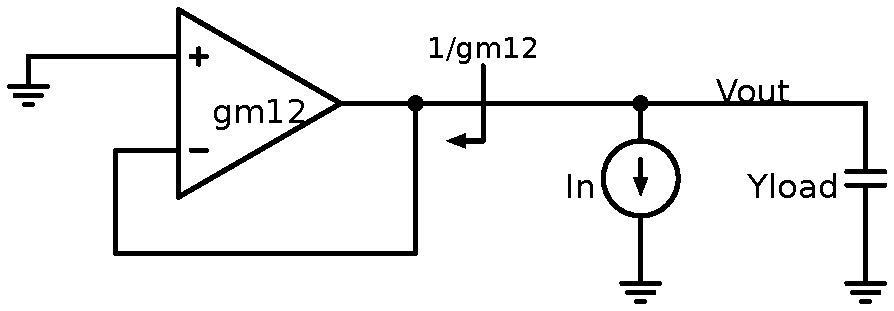
\includegraphics{index_files/mediabag/index_files/figure-pdf/fig-voltage-buffer-ota-noise-output-1.pdf}

}

\caption{\label{fig-voltage-buffer-ota-noise}A voltage buffer redrawn
for noise analysis.}

\end{figure}%

\textsubscript{Source:
\href{https://iic-jku.github.io/analog-circuit-design/index.qmd.html}{Article
Notebook}}

We see that the feedback around the transconductor \(g_\mathrm{m12}\)
creates an impedance of \(1/g_\mathrm{m12}\). We can now calculate the
effective load conductance of \[
Y'_\mathrm{load} = g_\mathrm{ds2} + g_\mathrm{ds4} + s C_\mathrm{load} + g_\mathrm{m12} \approx g_\mathrm{m12} + s C_\mathrm{load}.
\]

The output noise voltage is then (using Equation~\ref{eq-mosfet-noise})
\[
\overline{V_\mathrm{n,out}^2}(f) = \frac{\overline{I_\mathrm{n}^2}}{|Y'_\mathrm{load}|^2} = \frac{\overline{I_\mathrm{n}^2}}{g_\mathrm{m12}^2 + (2 \pi f C_\mathrm{load})2^2} = \frac{8 k T (\gamma_{12} g_\mathrm{m12} + \gamma_{34} g_\mathrm{m34})}{g_\mathrm{m12}^2 + (2 \pi f C_\mathrm{load})^2}.
\]

We can use the identity Equation~\ref{eq-integral-identity} to calculate
the rms output noise to
\begin{equation}\phantomsection\label{eq-basic-ota-output-noise}{
V_\mathrm{n,out,rms}^2 = \int_0^\infty \overline{V_\mathrm{n,out}^2}(f) df = \frac{k T}{C_\mathrm{load}} \left( 2 \gamma_{12} + 2 \gamma_{34} \frac{g_\mathrm{m34}}{g_\mathrm{m12}} \right).
}\end{equation}

Inspecting Equation~\ref{eq-basic-ota-output-noise} we can see that the
integrated output noise is the \(k T / C\) noise of the output load
capacitor, enhanced by the \(\gamma_{12}\) of the input differential
pair, plus a (smaller) contribution of the current mirror load
\(M_{3,4}\). Intuitevly, this result makes sense.

\begin{tcolorbox}[enhanced jigsaw, colback=white, bottomtitle=1mm, titlerule=0mm, toprule=.15mm, coltitle=black, title=\textcolor{quarto-callout-tip-color}{\faLightbulb}\hspace{0.5em}{Exercise: Derivation of 5T-OTA Performance}, opacityback=0, leftrule=.75mm, opacitybacktitle=0.6, left=2mm, toptitle=1mm, arc=.35mm, colframe=quarto-callout-tip-color-frame, breakable, colbacktitle=quarto-callout-tip-color!10!white, rightrule=.15mm, bottomrule=.15mm]

Please take your time and carefully go through the explanations and
derivations for the 5-transistor-OTA in
Section~\ref{sec-basic-ota-large-signal} and
Section~\ref{sec-basic-ota-small-signal}. Try to do the calculations
yourself; if you get stuck, review the previous chapters.

\end{tcolorbox}

\subsection{5T-OTA Sizing}\label{t-ota-sizing}

Outfitted with the governing equations derived in
Section~\ref{sec-basic-ota-small-signal} we can now size the MOSFETs in
the OTA, we remember that we have to size \(M_{1,2}\) and \(M_{3,4}\)
equally.

First, we need to select a proper \(g_\mathrm{m}/I_\mathrm{D}\) for the
MOSFET. Remembering Section~\ref{sec-gmid-method} we see that for the
input differential pair we should go for a large \(g_\mathrm{m}\), thus
we select a \(g_\mathrm{m}/I_\mathrm{D}= 10\). As \(g_\mathrm{ds}\) of
\(M_2\) could limit the dc gain (Equation~\ref{eq-simple-ota-gain-dc})
we go with a rather long \(L = 5\,\mu\text{m}\). For current sources a
small \(g_\mathrm{m}/I_\mathrm{D}\) is a good idea, so we start with
\(g_\mathrm{m}/I_\mathrm{D}=5\) (because we can not go too low because
of \(V_\mathrm{ds,sat}\)) and also an \(L = 5\,\mu\text{m}\).

\begin{tcolorbox}[enhanced jigsaw, colback=white, bottomtitle=1mm, titlerule=0mm, toprule=.15mm, coltitle=black, title=\textcolor{quarto-callout-tip-color}{\faLightbulb}\hspace{0.5em}{Exercise: 5T-OTA Sizing}, opacityback=0, leftrule=.75mm, opacitybacktitle=0.6, left=2mm, toptitle=1mm, arc=.35mm, colframe=quarto-callout-tip-color-frame, breakable, colbacktitle=quarto-callout-tip-color!10!white, rightrule=.15mm, bottomrule=.15mm]

Please size the 5T-OTA according to the previous
\(g_\mathrm{m}/I_\mathrm{D}\) and \(L\) suggestions. Please calculate
the \(W\) of \(M_{1-6}\) and the total supply current. Please check
wether gain error, total output noise, and turn-on settling is met with
the calculated devices sizes and bias currents.

\end{tcolorbox}

The sizing procedure and its calculation are best performed in a Jupyter
notebook, as we can easily look up the exact data from the pre-computed
tables:

\begin{tcolorbox}[enhanced jigsaw, colback=white, bottomtitle=1mm, titlerule=0mm, toprule=.15mm, coltitle=black, title=\textcolor{quarto-callout-tip-color}{\faLightbulb}\hspace{0.5em}{Solution: 5T-OTA Sizing}, opacityback=0, leftrule=.75mm, opacitybacktitle=0.6, left=2mm, toptitle=1mm, arc=.35mm, colframe=quarto-callout-tip-color-frame, breakable, colbacktitle=quarto-callout-tip-color!10!white, rightrule=.15mm, bottomrule=.15mm]

\section{Sizing for Basic 5T-OTA}\label{sizing-for-basic-5t-ota}

\textbf{Copyright 2024 Harald Pretl}

Licensed under the Apache License, Version 2.0 (the ``License''); you
may not use this file except in compliance with the License. You may
obtain a copy of the License at
http://www.apache.org/licenses/LICENSE-2.0

\begin{Shaded}
\begin{Highlighting}[]
\CommentTok{\# Read table data}
\ImportTok{from}\NormalTok{ pygmid }\ImportTok{import}\NormalTok{ Lookup }\ImportTok{as}\NormalTok{ lk}
\ImportTok{import}\NormalTok{ numpy }\ImportTok{as}\NormalTok{ np}
\NormalTok{lv\_nmos }\OperatorTok{=}\NormalTok{ lk(}\StringTok{\textquotesingle{}sg13\_lv\_nmos.mat\textquotesingle{}}\NormalTok{)}
\NormalTok{lv\_pmos }\OperatorTok{=}\NormalTok{ lk(}\StringTok{\textquotesingle{}sg13\_lv\_pmos.mat\textquotesingle{}}\NormalTok{)}
\CommentTok{\# List of parameters: VGS, VDS, VSB, L, W, NFING, ID, VT, GM, GMB, GDS, CGG, CGB, CGD, CGS, CDD, CSS, STH, SFL}
\CommentTok{\# If not specified, minimum L, VDS=max(vgs)/2=0.9 and VSB=0 are used }
\end{Highlighting}
\end{Shaded}

\begin{Shaded}
\begin{Highlighting}[]
\CommentTok{\# Define the given parameters as taken from the specification table or inital guesses}
\NormalTok{c\_load }\OperatorTok{=} \FloatTok{50e{-}15}
\NormalTok{gm\_id\_m12 }\OperatorTok{=} \DecValTok{10}
\NormalTok{gm\_id\_m34 }\OperatorTok{=} \DecValTok{5}
\NormalTok{gm\_id\_m56 }\OperatorTok{=} \DecValTok{5}
\NormalTok{l\_12 }\OperatorTok{=} \DecValTok{5}
\NormalTok{l\_34 }\OperatorTok{=} \DecValTok{5}
\NormalTok{l\_56 }\OperatorTok{=} \DecValTok{5}
\NormalTok{f\_bw }\OperatorTok{=} \FloatTok{10e6}
\NormalTok{i\_total\_limit }\OperatorTok{=} \FloatTok{10e{-}6}
\NormalTok{i\_bias\_in }\OperatorTok{=} \FloatTok{20e{-}6}
\NormalTok{output\_voltage }\OperatorTok{=} \FloatTok{1.3}
\NormalTok{vin\_min }\OperatorTok{=} \FloatTok{0.7}
\NormalTok{vin\_max }\OperatorTok{=} \FloatTok{0.9}
\NormalTok{vdd\_min }\OperatorTok{=} \FloatTok{1.45}
\NormalTok{vdd\_max }\OperatorTok{=} \FloatTok{1.55}
\end{Highlighting}
\end{Shaded}

\begin{Shaded}
\begin{Highlighting}[]
\CommentTok{\# We get the required gm of M1/2 from the bandwidth requirement}
\CommentTok{\# We add a factor of 3 to allow for PVT variation plus additional MOSFET parasitic loading}
\NormalTok{gm\_m12 }\OperatorTok{=}\NormalTok{ f\_bw }\OperatorTok{*} \DecValTok{3} \OperatorTok{*} \DecValTok{4}\OperatorTok{*}\NormalTok{np.pi}\OperatorTok{*}\NormalTok{c\_load}
\BuiltInTok{print}\NormalTok{(}\StringTok{\textquotesingle{}gm12 =\textquotesingle{}}\NormalTok{, gm\_m12}\OperatorTok{/}\FloatTok{1e{-}3}\NormalTok{, }\StringTok{\textquotesingle{}mS\textquotesingle{}}\NormalTok{)}
\end{Highlighting}
\end{Shaded}

\begin{verbatim}
gm12 = 0.01884955592153876 mS
\end{verbatim}

\begin{Shaded}
\begin{Highlighting}[]
\CommentTok{\# Since we know gm12 and the gmid we can calculate the bias current}
\NormalTok{id\_m12 }\OperatorTok{=}\NormalTok{ gm\_m12 }\OperatorTok{/}\NormalTok{ gm\_id\_m12}
\NormalTok{i\_total }\OperatorTok{=} \DecValTok{2}\OperatorTok{*}\NormalTok{id\_m12}
\BuiltInTok{print}\NormalTok{(}\StringTok{\textquotesingle{}i\_total (exact) =\textquotesingle{}}\NormalTok{, i\_total}\OperatorTok{/}\FloatTok{1e{-}6}\NormalTok{, }\StringTok{\textquotesingle{}µA\textquotesingle{}}\NormalTok{)}
\CommentTok{\# we round to 0.5µA bias currents}
\NormalTok{i\_total }\OperatorTok{=} \BuiltInTok{max}\NormalTok{(}\BuiltInTok{round}\NormalTok{(i\_total }\OperatorTok{/} \FloatTok{1e{-}6} \OperatorTok{*} \DecValTok{2}\NormalTok{) }\OperatorTok{/} \DecValTok{2} \OperatorTok{*} \FloatTok{1e{-}6}\NormalTok{, }\FloatTok{0.5e{-}6}\NormalTok{)}
\NormalTok{id\_m12 }\OperatorTok{=}\NormalTok{ i\_total}\OperatorTok{/}\DecValTok{2}

\BuiltInTok{print}\NormalTok{(}\StringTok{\textquotesingle{}i\_total (rounded) =\textquotesingle{}}\NormalTok{, i\_total}\OperatorTok{/}\FloatTok{1e{-}6}\NormalTok{, }\StringTok{\textquotesingle{}µA\textquotesingle{}}\NormalTok{)}
\ControlFlowTok{if}\NormalTok{ i\_total }\OperatorTok{\textless{}}\NormalTok{ i\_total\_limit:}
    \BuiltInTok{print}\NormalTok{(}\StringTok{\textquotesingle{}[info] power consumption target is met!\textquotesingle{}}\NormalTok{)}
\ControlFlowTok{else}\NormalTok{:}
    \BuiltInTok{print}\NormalTok{(}\StringTok{\textquotesingle{}[info] power consumption target is NOT met!\textquotesingle{}}\NormalTok{) }
\end{Highlighting}
\end{Shaded}

\begin{verbatim}
i_total (exact) = 3.7699111843077517 µA
i_total (rounded) = 4.0 µA
[info] power consumption target is met!
\end{verbatim}

\begin{Shaded}
\begin{Highlighting}[]
\CommentTok{\# We calculate the dc gain}
\NormalTok{gm\_gds\_m12 }\OperatorTok{=}\NormalTok{ lv\_nmos.lookup(}\StringTok{\textquotesingle{}GM\_GDS\textquotesingle{}}\NormalTok{, GM\_ID}\OperatorTok{=}\NormalTok{gm\_id\_m12, L}\OperatorTok{=}\NormalTok{l\_12, VDS}\OperatorTok{=}\FloatTok{0.75}\NormalTok{, VSB}\OperatorTok{=}\DecValTok{0}\NormalTok{)}
\NormalTok{gm\_gds\_m34 }\OperatorTok{=}\NormalTok{ lv\_pmos.lookup(}\StringTok{\textquotesingle{}GM\_GDS\textquotesingle{}}\NormalTok{, GM\_ID}\OperatorTok{=}\NormalTok{gm\_id\_m34, L}\OperatorTok{=}\NormalTok{l\_34, VDS}\OperatorTok{=}\FloatTok{0.75}\NormalTok{, VSB}\OperatorTok{=}\DecValTok{0}\NormalTok{)}

\NormalTok{gds\_m12 }\OperatorTok{=}\NormalTok{ gm\_m12 }\OperatorTok{/}\NormalTok{ gm\_gds\_m12}
\NormalTok{gm\_m34 }\OperatorTok{=}\NormalTok{ gm\_id\_m34 }\OperatorTok{*}\NormalTok{ i\_total}\OperatorTok{/}\DecValTok{2}
\NormalTok{gds\_m34 }\OperatorTok{=}\NormalTok{ gm\_m34 }\OperatorTok{/}\NormalTok{ gm\_gds\_m34}

\NormalTok{a0 }\OperatorTok{=}\NormalTok{ gm\_m12 }\OperatorTok{/}\NormalTok{ (gds\_m12 }\OperatorTok{+}\NormalTok{ gds\_m34)}
\BuiltInTok{print}\NormalTok{(}\StringTok{\textquotesingle{}a0 =\textquotesingle{}}\NormalTok{, }\DecValTok{20}\OperatorTok{*}\NormalTok{np.log10(a0), }\StringTok{\textquotesingle{}dB\textquotesingle{}}\NormalTok{)}
\end{Highlighting}
\end{Shaded}

\begin{verbatim}
a0 = 34.78458740352468 dB
\end{verbatim}

\begin{Shaded}
\begin{Highlighting}[]
\CommentTok{\# We calculate the MOSFET capacitance which adds to Cload, to see the impact on the BW}
\NormalTok{gm\_cgs\_m12 }\OperatorTok{=}\NormalTok{ lv\_nmos.lookup(}\StringTok{\textquotesingle{}GM\_CGS\textquotesingle{}}\NormalTok{, GM\_ID}\OperatorTok{=}\NormalTok{gm\_id\_m12, L}\OperatorTok{=}\NormalTok{l\_12, VDS}\OperatorTok{=}\FloatTok{0.75}\NormalTok{, VSB}\OperatorTok{=}\DecValTok{0}\NormalTok{)}
\NormalTok{gm\_cdd\_m12 }\OperatorTok{=}\NormalTok{ lv\_nmos.lookup(}\StringTok{\textquotesingle{}GM\_CDD\textquotesingle{}}\NormalTok{, GM\_ID}\OperatorTok{=}\NormalTok{gm\_id\_m12, L}\OperatorTok{=}\NormalTok{l\_12, VDS}\OperatorTok{=}\FloatTok{0.75}\NormalTok{, VSB}\OperatorTok{=}\DecValTok{0}\NormalTok{)}
\NormalTok{gm\_cdd\_m34 }\OperatorTok{=}\NormalTok{ lv\_pmos.lookup(}\StringTok{\textquotesingle{}GM\_CDD\textquotesingle{}}\NormalTok{, GM\_ID}\OperatorTok{=}\NormalTok{gm\_id\_m34, L}\OperatorTok{=}\NormalTok{l\_34, VDS}\OperatorTok{=}\FloatTok{0.75}\NormalTok{, VSB}\OperatorTok{=}\DecValTok{0}\NormalTok{)}

\NormalTok{c\_load\_parasitic }\OperatorTok{=} \BuiltInTok{abs}\NormalTok{(gm\_m12}\OperatorTok{/}\NormalTok{gm\_cgs\_m12) }\OperatorTok{+} \BuiltInTok{abs}\NormalTok{(gm\_m12}\OperatorTok{/}\NormalTok{gm\_cdd\_m12) }\OperatorTok{+} \BuiltInTok{abs}\NormalTok{(gm\_m34}\OperatorTok{/}\NormalTok{gm\_cdd\_m34)}
\BuiltInTok{print}\NormalTok{(}\StringTok{\textquotesingle{}additional load capacitance =\textquotesingle{}}\NormalTok{, c\_load\_parasitic}\OperatorTok{/}\FloatTok{1e{-}15}\NormalTok{, }\StringTok{\textquotesingle{}fF\textquotesingle{}}\NormalTok{)}

\NormalTok{f\_bw }\OperatorTok{=}\NormalTok{ gm\_m12 }\OperatorTok{/}\NormalTok{ (}\DecValTok{4}\OperatorTok{*}\NormalTok{np.pi }\OperatorTok{*}\NormalTok{ (c\_load }\OperatorTok{+}\NormalTok{ c\_load\_parasitic))}
\BuiltInTok{print}\NormalTok{(}\StringTok{\textquotesingle{}{-}3dB bandwidth incl. parasitics =\textquotesingle{}}\NormalTok{, f\_bw}\OperatorTok{/}\FloatTok{1e6}\NormalTok{, }\StringTok{\textquotesingle{}MHz\textquotesingle{}}\NormalTok{)}
\end{Highlighting}
\end{Shaded}

\begin{verbatim}
additional load capacitance = 54.92854674560976 fF
-3dB bandwidth incl. parasitics = 14.295442437000684 MHz
\end{verbatim}

\begin{Shaded}
\begin{Highlighting}[]
\CommentTok{\# We can now look up the VGS of the MOSFET}
\NormalTok{vgs\_m12 }\OperatorTok{=}\NormalTok{ lv\_nmos.look\_upVGS(GM\_ID}\OperatorTok{=}\NormalTok{gm\_id\_m12, L}\OperatorTok{=}\NormalTok{l\_12, VDS}\OperatorTok{=}\FloatTok{0.75}\NormalTok{, VSB}\OperatorTok{=}\FloatTok{0.0}\NormalTok{)}
\NormalTok{vgs\_m34 }\OperatorTok{=}\NormalTok{ lv\_pmos.look\_upVGS(GM\_ID}\OperatorTok{=}\NormalTok{gm\_id\_m34, L}\OperatorTok{=}\NormalTok{l\_34, VDS}\OperatorTok{=}\FloatTok{0.75}\NormalTok{, VSB}\OperatorTok{=}\FloatTok{0.0}\NormalTok{) }
\NormalTok{vgs\_m56 }\OperatorTok{=}\NormalTok{ lv\_nmos.look\_upVGS(GM\_ID}\OperatorTok{=}\NormalTok{gm\_id\_m56, L}\OperatorTok{=}\NormalTok{l\_56, VDS}\OperatorTok{=}\FloatTok{0.75}\NormalTok{, VSB}\OperatorTok{=}\FloatTok{0.0}\NormalTok{) }

\BuiltInTok{print}\NormalTok{(}\StringTok{\textquotesingle{}vgs\_12 =\textquotesingle{}}\NormalTok{, vgs\_m12, }\StringTok{\textquotesingle{}V\textquotesingle{}}\NormalTok{)}
\BuiltInTok{print}\NormalTok{(}\StringTok{\textquotesingle{}vgs\_34 =\textquotesingle{}}\NormalTok{, vgs\_m34, }\StringTok{\textquotesingle{}V\textquotesingle{}}\NormalTok{)}
\BuiltInTok{print}\NormalTok{(}\StringTok{\textquotesingle{}vgs\_56 =\textquotesingle{}}\NormalTok{, vgs\_m56, }\StringTok{\textquotesingle{}V\textquotesingle{}}\NormalTok{)}
\end{Highlighting}
\end{Shaded}

\begin{verbatim}
vgs_12 = 0.36710119710062455 V
vgs_34 = 0.7287454603526495 V
vgs_56 = 0.5912200307058603 V
\end{verbatim}

\begin{Shaded}
\begin{Highlighting}[]
\CommentTok{\# Calculate settling time due to slewing with the calculated bias current}
\NormalTok{t\_slew }\OperatorTok{=}\NormalTok{ (c\_load }\OperatorTok{+}\NormalTok{ c\_load\_parasitic) }\OperatorTok{*}\NormalTok{ output\_voltage }\OperatorTok{/}\NormalTok{ i\_total}
\BuiltInTok{print}\NormalTok{(}\StringTok{\textquotesingle{}slewing time =\textquotesingle{}}\NormalTok{, t\_slew}\OperatorTok{/}\FloatTok{1e{-}6}\NormalTok{, }\StringTok{\textquotesingle{}µs\textquotesingle{}}\NormalTok{)}
\NormalTok{t\_settle }\OperatorTok{=} \DecValTok{5}\OperatorTok{/}\NormalTok{(}\DecValTok{2}\OperatorTok{*}\NormalTok{np.pi}\OperatorTok{*}\NormalTok{f\_bw)}
\BuiltInTok{print}\NormalTok{(}\StringTok{\textquotesingle{}settling time =\textquotesingle{}}\NormalTok{, t\_settle}\OperatorTok{/}\FloatTok{1e{-}6}\NormalTok{, }\StringTok{\textquotesingle{}µs\textquotesingle{}}\NormalTok{)}
\end{Highlighting}
\end{Shaded}

\begin{verbatim}
slewing time = 0.034101777692323185 µs
settling time = 0.055666322953376014 µs
\end{verbatim}

\begin{Shaded}
\begin{Highlighting}[]
\CommentTok{\# Calculate voltage gain error}
\NormalTok{gain\_error }\OperatorTok{=}\NormalTok{ a0 }\OperatorTok{/}\NormalTok{ (}\DecValTok{1} \OperatorTok{+}\NormalTok{ a0)}
\BuiltInTok{print}\NormalTok{(}\StringTok{\textquotesingle{}voltage gain error =\textquotesingle{}}\NormalTok{, (gain\_error}\OperatorTok{{-}}\DecValTok{1}\NormalTok{)}\OperatorTok{*}\DecValTok{100}\NormalTok{, }\StringTok{\textquotesingle{}\%\textquotesingle{}}\NormalTok{)}
\end{Highlighting}
\end{Shaded}

\begin{verbatim}
voltage gain error = -1.7902967715882068 %
\end{verbatim}

\begin{Shaded}
\begin{Highlighting}[]
\CommentTok{\# Calculate total rms output noise}
\NormalTok{sth\_m12 }\OperatorTok{=}\NormalTok{ lv\_nmos.lookup(}\StringTok{\textquotesingle{}STH\_GM\textquotesingle{}}\NormalTok{, VGS}\OperatorTok{=}\NormalTok{vgs\_m12, L}\OperatorTok{=}\NormalTok{l\_12, VDS}\OperatorTok{=}\FloatTok{0.75}\NormalTok{, VSB}\OperatorTok{=}\DecValTok{0}\NormalTok{) }\OperatorTok{*}\NormalTok{ gm\_m12}
\NormalTok{gamma\_m12 }\OperatorTok{=}\NormalTok{ sth\_m12}\OperatorTok{/}\NormalTok{(}\DecValTok{4}\OperatorTok{*}\FloatTok{1.38e{-}23}\OperatorTok{*}\DecValTok{300}\OperatorTok{*}\NormalTok{gm\_m12)}

\NormalTok{sth\_m34 }\OperatorTok{=}\NormalTok{ lv\_pmos.lookup(}\StringTok{\textquotesingle{}STH\_GM\textquotesingle{}}\NormalTok{, VGS}\OperatorTok{=}\NormalTok{vgs\_m34, L}\OperatorTok{=}\NormalTok{l\_34, VDS}\OperatorTok{=}\FloatTok{0.75}\NormalTok{, VSB}\OperatorTok{=}\DecValTok{0}\NormalTok{) }\OperatorTok{*}\NormalTok{ gm\_m34}
\NormalTok{gamma\_m34 }\OperatorTok{=}\NormalTok{ sth\_m34}\OperatorTok{/}\NormalTok{(}\DecValTok{4}\OperatorTok{*}\FloatTok{1.38e{-}23}\OperatorTok{*}\DecValTok{300}\OperatorTok{*}\NormalTok{gm\_m34)}

\NormalTok{output\_noise\_rms }\OperatorTok{=} \FloatTok{1.38e{-}23}\OperatorTok{*}\DecValTok{300} \OperatorTok{/}\NormalTok{ (c\_load }\OperatorTok{+}\NormalTok{ c\_load\_parasitic) }\OperatorTok{*}\NormalTok{ (}\DecValTok{2}\OperatorTok{*}\NormalTok{gamma\_m12 }\OperatorTok{+} \DecValTok{2}\OperatorTok{*}\NormalTok{gamma\_m34 }\OperatorTok{*}\NormalTok{ gm\_m34}\OperatorTok{/}\NormalTok{gm\_m12)}
\BuiltInTok{print}\NormalTok{(}\StringTok{\textquotesingle{}output noise (rms) =\textquotesingle{}}\NormalTok{, output\_noise\_rms}\OperatorTok{/}\FloatTok{1e{-}6}\NormalTok{, }\StringTok{\textquotesingle{}µV\textquotesingle{}}\NormalTok{)}
\end{Highlighting}
\end{Shaded}

\begin{verbatim}
output noise (rms) = 0.12543377043178017 µV
\end{verbatim}

\begin{Shaded}
\begin{Highlighting}[]
\CommentTok{\# Calculate all widths}
\NormalTok{id\_w\_m12 }\OperatorTok{=}\NormalTok{ lv\_nmos.lookup(}\StringTok{\textquotesingle{}ID\_W\textquotesingle{}}\NormalTok{, GM\_ID}\OperatorTok{=}\NormalTok{gm\_id\_m12, L}\OperatorTok{=}\NormalTok{l\_12, VDS}\OperatorTok{=}\NormalTok{vgs\_m12, VSB}\OperatorTok{=}\DecValTok{0}\NormalTok{)}
\NormalTok{w\_12 }\OperatorTok{=}\NormalTok{ id\_m12 }\OperatorTok{/}\NormalTok{ id\_w\_m12}
\NormalTok{w\_12\_round }\OperatorTok{=} \BuiltInTok{max}\NormalTok{(}\BuiltInTok{round}\NormalTok{(w\_12}\OperatorTok{*}\DecValTok{2}\NormalTok{)}\OperatorTok{/}\DecValTok{2}\NormalTok{, }\FloatTok{0.5}\NormalTok{)}
\BuiltInTok{print}\NormalTok{(}\StringTok{\textquotesingle{}M1/2 W =\textquotesingle{}}\NormalTok{, w\_12, }\StringTok{\textquotesingle{}um, rounded W =\textquotesingle{}}\NormalTok{, w\_12\_round, }\StringTok{\textquotesingle{}um\textquotesingle{}}\NormalTok{)}

\NormalTok{id\_m34 }\OperatorTok{=}\NormalTok{ id\_m12}
\NormalTok{id\_w\_m34 }\OperatorTok{=}\NormalTok{ lv\_pmos.lookup(}\StringTok{\textquotesingle{}ID\_W\textquotesingle{}}\NormalTok{, GM\_ID}\OperatorTok{=}\NormalTok{gm\_id\_m34, L}\OperatorTok{=}\NormalTok{l\_34, VDS}\OperatorTok{=}\NormalTok{vgs\_m34, VSB}\OperatorTok{=}\DecValTok{0}\NormalTok{)}
\NormalTok{w\_34 }\OperatorTok{=}\NormalTok{ id\_m34 }\OperatorTok{/}\NormalTok{ id\_w\_m34}
\NormalTok{w\_34\_round }\OperatorTok{=} \BuiltInTok{max}\NormalTok{(}\BuiltInTok{round}\NormalTok{(w\_34}\OperatorTok{*}\DecValTok{2}\NormalTok{)}\OperatorTok{/}\DecValTok{2}\NormalTok{, }\FloatTok{0.5}\NormalTok{) }
\BuiltInTok{print}\NormalTok{(}\StringTok{\textquotesingle{}M3/4 W =\textquotesingle{}}\NormalTok{, w\_34, }\StringTok{\textquotesingle{}um, rounded W =\textquotesingle{}}\NormalTok{, w\_34\_round, }\StringTok{\textquotesingle{}um\textquotesingle{}}\NormalTok{)}

\NormalTok{id\_w\_m5 }\OperatorTok{=}\NormalTok{ lv\_nmos.lookup(}\StringTok{\textquotesingle{}ID\_W\textquotesingle{}}\NormalTok{, GM\_ID}\OperatorTok{=}\NormalTok{gm\_id\_m56, L}\OperatorTok{=}\NormalTok{l\_56, VDS}\OperatorTok{=}\NormalTok{vgs\_m56, VSB}\OperatorTok{=}\DecValTok{0}\NormalTok{)}
\NormalTok{w\_5 }\OperatorTok{=}\NormalTok{ i\_total }\OperatorTok{/}\NormalTok{ id\_w\_m5}
\NormalTok{w\_5\_round }\OperatorTok{=} \BuiltInTok{max}\NormalTok{(}\BuiltInTok{round}\NormalTok{(w\_5}\OperatorTok{*}\DecValTok{2}\NormalTok{)}\OperatorTok{/}\DecValTok{2}\NormalTok{, }\FloatTok{0.5}\NormalTok{)}
\BuiltInTok{print}\NormalTok{(}\StringTok{\textquotesingle{}M5 W =\textquotesingle{}}\NormalTok{, w\_5, }\StringTok{\textquotesingle{}um, rounded W =\textquotesingle{}}\NormalTok{, w\_5\_round, }\StringTok{\textquotesingle{}um\textquotesingle{}}\NormalTok{)}
\NormalTok{w\_6 }\OperatorTok{=}\NormalTok{ w\_5\_round }\OperatorTok{*}\NormalTok{ i\_bias\_in }\OperatorTok{/}\NormalTok{ i\_total}
\BuiltInTok{print}\NormalTok{(}\StringTok{\textquotesingle{}M6 W =\textquotesingle{}}\NormalTok{, w\_6, }\StringTok{\textquotesingle{}um\textquotesingle{}}\NormalTok{)}
\end{Highlighting}
\end{Shaded}

\begin{verbatim}
M1/2 W = 1.7713641972645868 um, rounded W = 2.0 um
M3/4 W = 1.641014110777885 um, rounded W = 1.5 um
M5 W = 0.7351148286825442 um, rounded W = 0.5 um
M6 W = 2.5000000000000004 um
\end{verbatim}

\begin{Shaded}
\begin{Highlighting}[]
\CommentTok{\# Print out final design values}
\BuiltInTok{print}\NormalTok{(}\StringTok{\textquotesingle{}5T{-}OTA dimensioning:\textquotesingle{}}\NormalTok{)}
\BuiltInTok{print}\NormalTok{(}\StringTok{\textquotesingle{}{-}{-}{-}{-}{-}{-}{-}{-}{-}{-}{-}{-}{-}{-}{-}{-}{-}{-}{-}{-}\textquotesingle{}}\NormalTok{)}
\BuiltInTok{print}\NormalTok{(}\StringTok{\textquotesingle{}M1/2 W=\textquotesingle{}}\NormalTok{, w\_12\_round, }\StringTok{\textquotesingle{}, L=\textquotesingle{}}\NormalTok{, l\_12)}
\BuiltInTok{print}\NormalTok{(}\StringTok{\textquotesingle{}M3/4 W=\textquotesingle{}}\NormalTok{, w\_34\_round, }\StringTok{\textquotesingle{}, L=\textquotesingle{}}\NormalTok{, l\_34)}
\BuiltInTok{print}\NormalTok{(}\StringTok{\textquotesingle{}M5   W=\textquotesingle{}}\NormalTok{, w\_5\_round, }\StringTok{\textquotesingle{}, L=\textquotesingle{}}\NormalTok{, l\_56)}
\BuiltInTok{print}\NormalTok{(}\StringTok{\textquotesingle{}M6   W=\textquotesingle{}}\NormalTok{, w\_6, }\StringTok{\textquotesingle{}, L=\textquotesingle{}}\NormalTok{, l\_56)}
\BuiltInTok{print}\NormalTok{()}
\BuiltInTok{print}\NormalTok{(}\StringTok{\textquotesingle{}5T{-}OTA performance summary:\textquotesingle{}}\NormalTok{)}
\BuiltInTok{print}\NormalTok{(}\StringTok{\textquotesingle{}{-}{-}{-}{-}{-}{-}{-}{-}{-}{-}{-}{-}{-}{-}{-}{-}{-}{-}{-}{-}{-}{-}{-}{-}{-}{-}{-}\textquotesingle{}}\NormalTok{)}
\BuiltInTok{print}\NormalTok{(}\StringTok{\textquotesingle{}supply current =\textquotesingle{}}\NormalTok{, i\_total}\OperatorTok{/}\FloatTok{1e{-}6}\NormalTok{, }\StringTok{\textquotesingle{}µA\textquotesingle{}}\NormalTok{)}
\BuiltInTok{print}\NormalTok{(}\StringTok{\textquotesingle{}output noise =\textquotesingle{}}\NormalTok{, output\_noise\_rms}\OperatorTok{/}\FloatTok{1e{-}6}\NormalTok{, }\StringTok{\textquotesingle{}µVrms\textquotesingle{}}\NormalTok{)}
\BuiltInTok{print}\NormalTok{(}\StringTok{\textquotesingle{}voltage gain error =\textquotesingle{}}\NormalTok{, (gain\_error}\OperatorTok{{-}}\DecValTok{1}\NormalTok{)}\OperatorTok{*}\DecValTok{100}\NormalTok{, }\StringTok{\textquotesingle{}\%\textquotesingle{}}\NormalTok{)}
\BuiltInTok{print}\NormalTok{(}\StringTok{\textquotesingle{}{-}3dB bandwidth incl. parasitics =\textquotesingle{}}\NormalTok{, f\_bw}\OperatorTok{/}\FloatTok{1e6}\NormalTok{, }\StringTok{\textquotesingle{}MHz\textquotesingle{}}\NormalTok{)}
\BuiltInTok{print}\NormalTok{(}\StringTok{\textquotesingle{}turn{-}on time (slewing+settling) =\textquotesingle{}}\NormalTok{, (t\_slew}\OperatorTok{+}\NormalTok{t\_settle)}\OperatorTok{/}\FloatTok{1e{-}6}\NormalTok{, }\StringTok{\textquotesingle{}µs\textquotesingle{}}\NormalTok{)}
\BuiltInTok{print}\NormalTok{()}
\BuiltInTok{print}\NormalTok{(}\StringTok{\textquotesingle{}5T{-}OTA bias point check:\textquotesingle{}}\NormalTok{)}
\BuiltInTok{print}\NormalTok{(}\StringTok{\textquotesingle{}{-}{-}{-}{-}{-}{-}{-}{-}{-}{-}{-}{-}{-}{-}{-}{-}{-}{-}{-}{-}{-}{-}{-}{-}\textquotesingle{}}\NormalTok{)}
\BuiltInTok{print}\NormalTok{(}\StringTok{\textquotesingle{}headroom M1 =\textquotesingle{}}\NormalTok{, vdd\_min}\OperatorTok{{-}}\NormalTok{vgs\_m34}\OperatorTok{+}\NormalTok{vgs\_m12}\OperatorTok{{-}}\NormalTok{vin\_max, }\StringTok{\textquotesingle{}V\textquotesingle{}}\NormalTok{)}
\BuiltInTok{print}\NormalTok{(}\StringTok{\textquotesingle{}headroom M4 =\textquotesingle{}}\NormalTok{, vdd\_min}\OperatorTok{{-}}\NormalTok{vin\_max, }\StringTok{\textquotesingle{}V\textquotesingle{}}\NormalTok{)}
\BuiltInTok{print}\NormalTok{(}\StringTok{\textquotesingle{}headroom M5 =\textquotesingle{}}\NormalTok{, vin\_min}\OperatorTok{{-}}\NormalTok{vgs\_m12, }\StringTok{\textquotesingle{}V\textquotesingle{}}\NormalTok{)}
\end{Highlighting}
\end{Shaded}

\begin{verbatim}
5T-OTA dimensioning:
--------------------
M1/2 W= 2.0 , L= 5
M3/4 W= 1.5 , L= 5
M5   W= 0.5 , L= 5
M6   W= 2.5000000000000004 , L= 5

5T-OTA performance summary:
---------------------------
supply current = 4.0 µA
output noise = 0.12543377043178017 µVrms
voltage gain error = -1.7902967715882068 %
-3dB bandwidth incl. parasitics = 14.295442437000684 MHz
turn-on time (slewing+settling) = 0.08976810064569919 µs

5T-OTA bias point check:
------------------------
headroom M1 = 0.188355736747975 V
headroom M4 = 0.5499999999999999 V
headroom M5 = 0.3328988028993754 V
\end{verbatim}

\textsubscript{Source:
\href{https://iic-jku.github.io/analog-circuit-design/sizing/sizing_basic_ota-preview.html\#cell-0}{Sizing
for Basic 5T-OTA}}

\end{tcolorbox}

\subsection{5T-OTA Simulation}\label{sec-basic-ota-simulation}

With the initial sizing of the MOSFETs of the 5T-OTA done, we can design
the 5T-OTA circuit and setup a simulation testbench to check the
performance parameters.

\begin{tcolorbox}[enhanced jigsaw, colback=white, bottomtitle=1mm, titlerule=0mm, toprule=.15mm, coltitle=black, title=\textcolor{quarto-callout-tip-color}{\faLightbulb}\hspace{0.5em}{Exercise: 5T-OTA Design and Testbench}, opacityback=0, leftrule=.75mm, opacitybacktitle=0.6, left=2mm, toptitle=1mm, arc=.35mm, colframe=quarto-callout-tip-color-frame, breakable, colbacktitle=quarto-callout-tip-color!10!white, rightrule=.15mm, bottomrule=.15mm]

Please design the circuit of the 5T-OTA. Put the OTA circuit in a
separate schematic, create a symbol for it, and use this symbol in a
testbench you create in Xschem for this 5T-OTA used as a voltage buffer
as schown in Figure~\ref{fig-voltage-buffer-ota}. Use typical conditions
for the simulation, and check how well the specification in
Table~\ref{tbl-voltage-buffer-spec} is met, and how well the derivations
in Section~\ref{sec-basic-ota-large-signal} and
Section~\ref{sec-basic-ota-small-signal} fit to the simulation results.

If you get stuck, you can find the testbench and 5T-OTA schematic
\href{./xschem/ota-5t_tb-ac.svg}{here} (for the small-signal analysis)
and \href{./xschem/ota-5t_tb-ac.svg}{here} (for the large-signal
settling simulation).

\end{tcolorbox}

\subsection{5T-OTA Simulation versus
PVT}\label{t-ota-simulation-versus-pvt}

As you have seen in Section~\ref{sec-basic-ota-simulation} running
simulations by hand is tedious. When we want to check the overall
performance, we have to run many simulations over various conditions:

\begin{enumerate}
\def\labelenumi{\arabic{enumi}.}
\tightlist
\item
  The supply voltage of the circuit has tolerances, and thus we need to
  check the performance against this variation.
\item
  The temperature at which the circuit is operated is likely changing.
  Also the performance against this has to be verified.
\item
  When manufacturing the wafers random variations in various process
  parameters lead to changed parameters of the integrated circuit
  components. In order to check for this effect, wafer foundries provide
  model files which shall cover these manufacturing excursions.
  Simplified, this leads to a slower or faster MOSFET, and usually NMOS
  and PMOS are not correlated, so we have the process corners
  \textbf{SS}, \textbf{SF}, \textbf{TT}, \textbf{FS}, and \textbf{FF}.
  So far, we have only used the \textbf{TT} models in our simulations.
\end{enumerate}

The variations listed in the previous list are abbreviated as
\textbf{PVT} (process, voltage, temperature) variations. In order to
finalize a circuit all combinations of these (plus the variations in
operating conditions like input voltage) have to be simulated. As you
can imagine, this leads to a huge number of simulations, and simulation
results which have to be evaluated for pass/fail.

There are two options how to tackle this efficiently:

\begin{enumerate}
\def\labelenumi{\arabic{enumi}.}
\tightlist
\item
  As an experienced designer you have a very solid understanding of the
  circuit, plus based on the analytic equations you can identify which
  combination of operating conditions will lead to a worst case
  performance. Thus, you can drastically reduce the number of corners to
  simulate, and you run them by hand.
\item
  You are using a framework which highly automates this task of running
  a plethora of different simulations and evaluating the outcome. These
  frameworks are called simulation runners.
\end{enumerate}

Luckily, there are open-source versions of simulation runners available,
and we will use \href{https://github.com/efabless/cace}{CACE} in this
lecture. CACE is written in Python and allows to setup a datasheet in
\href{https://yaml.org}{YAML} which defines the simulation problem and
the performance parameters to evaluate against which limits. The
resulting simulations are then run in parallel and the simulation data
is evaluated and summarized in various forms.

There is a CACE setup available for our 5T-OTA. The
\href{./cace/voltage-buffer-ota.yaml}{datasheet} describes the operating
conditions and the simulations tasks. For each simulation a testbench
template is needed, \href{./cace/templates/ota-5t-ac.sch}{this one} is
used for ac simulations, \href{./cace/templates/ota-5t-noise.sch}{this
one} is used for noise simulation, and
\href{./cace/templates/ota-5t-tran.sch}{this one} is used for transient
simulation.

After a successul run, a documentation is automatically generated. The
result of a full run of this \href{./xschem/ota-5t.svg}{OTA design} is
presented here:

\begin{tcolorbox}[enhanced jigsaw, colback=white, bottomtitle=1mm, titlerule=0mm, toprule=.15mm, coltitle=black, title=\textcolor{quarto-callout-note-color}{\faInfo}\hspace{0.5em}{Note \ref*{nte-basic-ota-cace-result}: CACE Summary for 5T-OTA}, opacityback=0, leftrule=.75mm, opacitybacktitle=0.6, left=2mm, toptitle=1mm, arc=.35mm, colframe=quarto-callout-note-color-frame, breakable, colbacktitle=quarto-callout-note-color!10!white, rightrule=.15mm, bottomrule=.15mm]

\quartocalloutnte{nte-basic-ota-cace-result} 

\section{CACE Summary for ota-5t}\label{cace-summary-for-ota-5t}

\textbf{netlist source}: schematic

\begin{longtable}[]{@{}
  >{\raggedright\arraybackslash}p{(\columnwidth - 18\tabcolsep) * \real{0.1550}}
  >{\raggedright\arraybackslash}p{(\columnwidth - 18\tabcolsep) * \real{0.1550}}
  >{\raggedright\arraybackslash}p{(\columnwidth - 18\tabcolsep) * \real{0.1163}}
  >{\raggedleft\arraybackslash}p{(\columnwidth - 18\tabcolsep) * \real{0.0775}}
  >{\raggedleft\arraybackslash}p{(\columnwidth - 18\tabcolsep) * \real{0.0930}}
  >{\raggedleft\arraybackslash}p{(\columnwidth - 18\tabcolsep) * \real{0.0775}}
  >{\raggedleft\arraybackslash}p{(\columnwidth - 18\tabcolsep) * \real{0.0930}}
  >{\raggedleft\arraybackslash}p{(\columnwidth - 18\tabcolsep) * \real{0.0775}}
  >{\raggedleft\arraybackslash}p{(\columnwidth - 18\tabcolsep) * \real{0.0930}}
  >{\centering\arraybackslash}p{(\columnwidth - 18\tabcolsep) * \real{0.0620}}@{}}
\toprule\noalign{}
\begin{minipage}[b]{\linewidth}\raggedright
Parameter
\end{minipage} & \begin{minipage}[b]{\linewidth}\raggedright
Tool
\end{minipage} & \begin{minipage}[b]{\linewidth}\raggedright
Result
\end{minipage} & \begin{minipage}[b]{\linewidth}\raggedleft
Min Limit
\end{minipage} & \begin{minipage}[b]{\linewidth}\raggedleft
Min Value
\end{minipage} & \begin{minipage}[b]{\linewidth}\raggedleft
Typ Target
\end{minipage} & \begin{minipage}[b]{\linewidth}\raggedleft
Typ Value
\end{minipage} & \begin{minipage}[b]{\linewidth}\raggedleft
Max Limit
\end{minipage} & \begin{minipage}[b]{\linewidth}\raggedleft
Max Value
\end{minipage} & \begin{minipage}[b]{\linewidth}\centering
Status
\end{minipage} \\
\midrule\noalign{}
\endhead
\bottomrule\noalign{}
\endlastfoot
Output voltage ratio & ngspice & gain & 0.97 V/V & 0.987 V/V & any &
1.000 V/V & 1.03 V/V & 1.006 V/V & Pass ✅ \\
Bandwidth & ngspice & bw & 10e6 Hz & 15551000.000 Hz & any &
26912100.000 Hz & any & 34051700.000 Hz & Pass ✅ \\
Output noise & ngspice & noise & any & 0.308 mV & any & 0.371 mV & 1 mV
& 0.455 mV & Pass ✅ \\
Settling time & ngspice & tsettle & any & 0.135 us & any & 0.142 us & 10
us & 0.155 us & Pass ✅ \\
\end{longtable}

\subsection{Plots}\label{plots}

\subsection{gain\_vs\_temp}\label{gain_vs_temp}

\begin{figure}[H]

{\centering 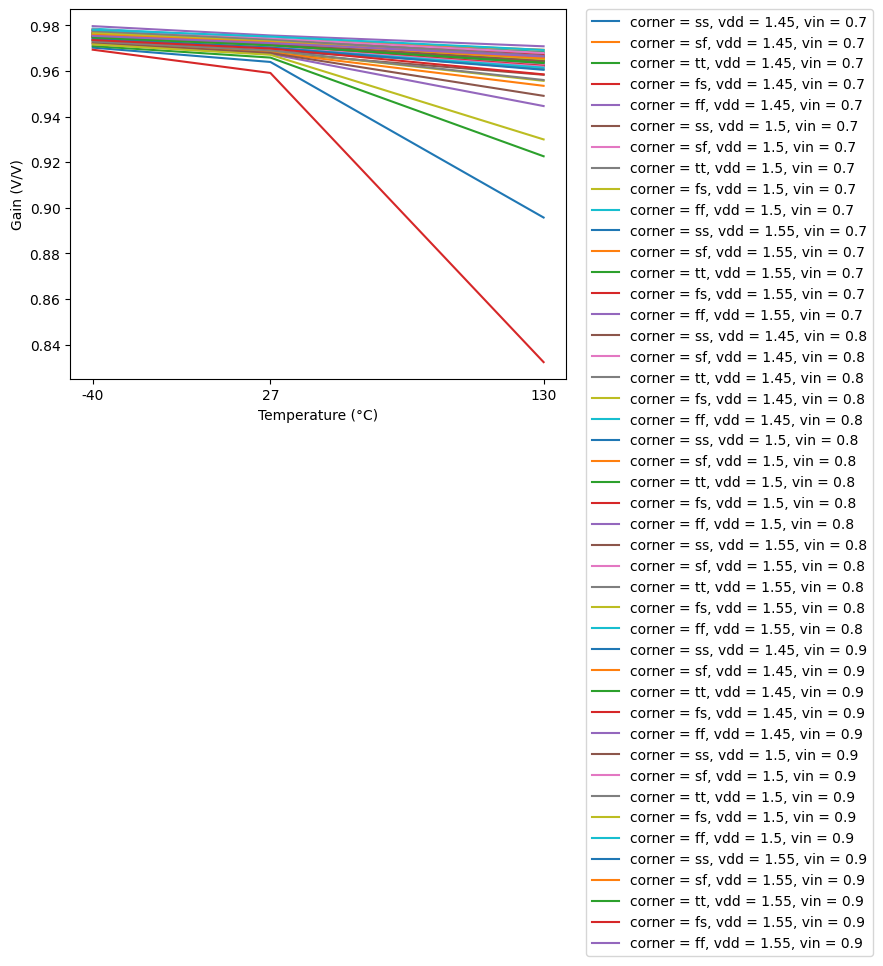
\includegraphics{./cace/_docs/ota-5t/schematic/gain_vs_temp.png}

}

\caption{gain\_vs\_temp}

\end{figure}%

\subsection{gain\_vs\_vin}\label{gain_vs_vin}

\begin{figure}[H]

{\centering 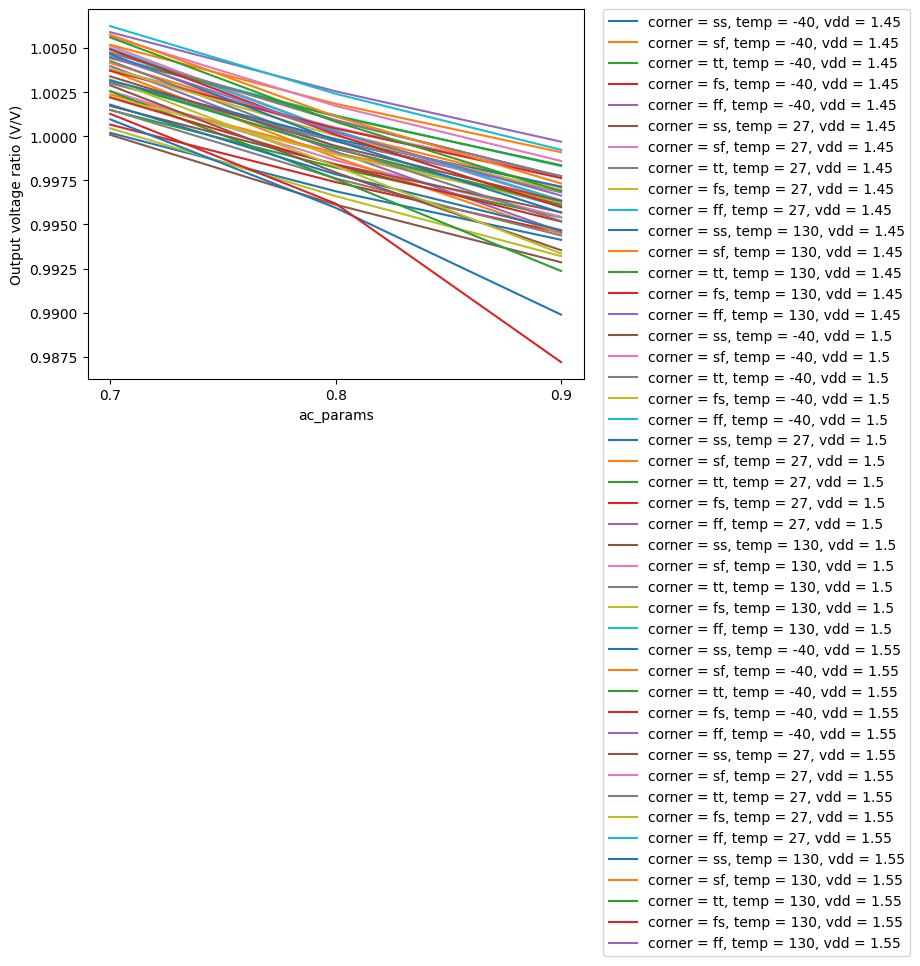
\includegraphics{./cace/_docs/ota-5t/schematic/gain_vs_vin.png}

}

\caption{gain\_vs\_vin}

\end{figure}%

\subsection{gain\_vs\_vdd}\label{gain_vs_vdd}

\begin{figure}[H]

{\centering 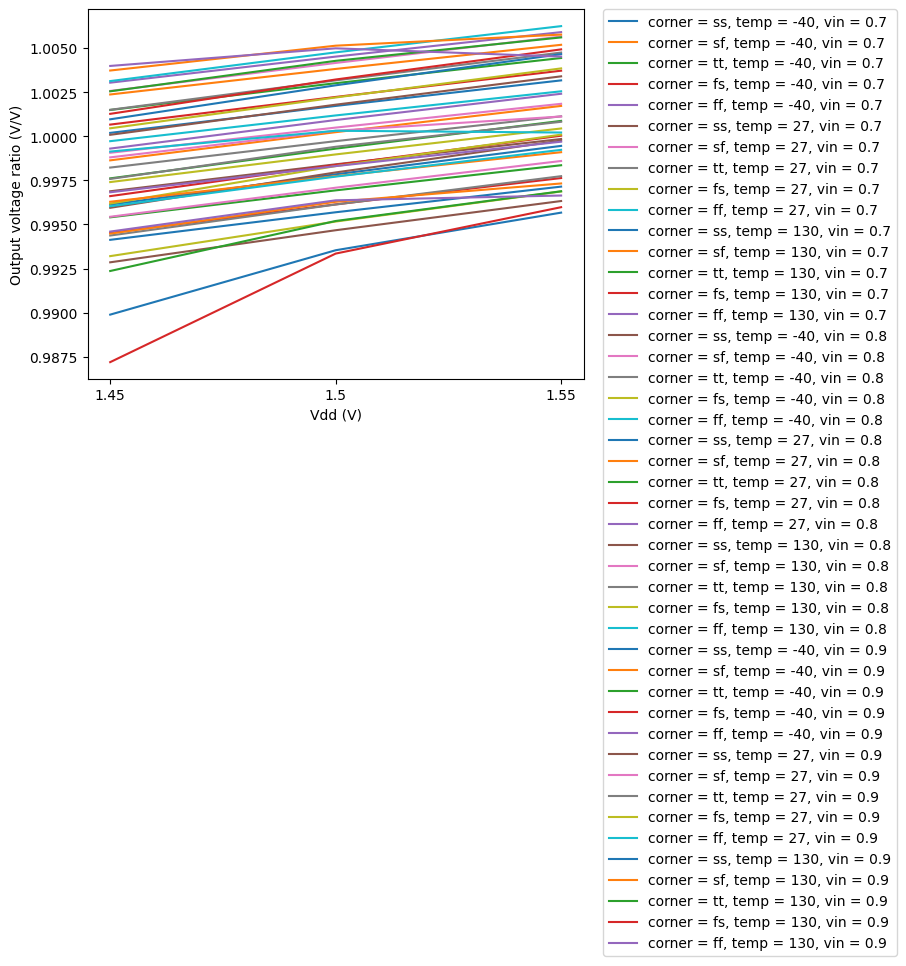
\includegraphics{./cace/_docs/ota-5t/schematic/gain_vs_vdd.png}

}

\caption{gain\_vs\_vdd}

\end{figure}%

\subsection{gain\_vs\_corner}\label{gain_vs_corner}

\begin{figure}[H]

{\centering 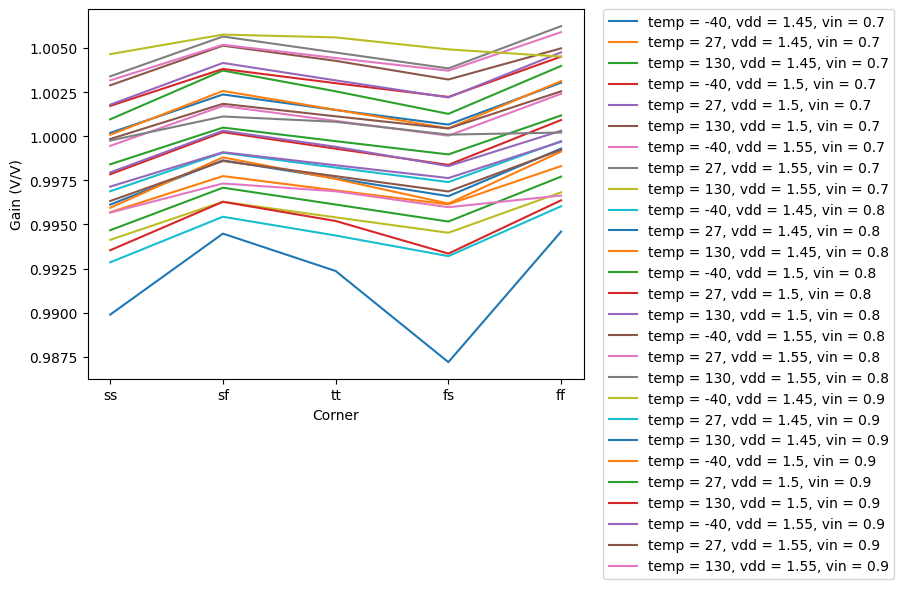
\includegraphics{./cace/_docs/ota-5t/schematic/gain_vs_corner.png}

}

\caption{gain\_vs\_corner}

\end{figure}%

\subsection{bw\_vs\_temp}\label{bw_vs_temp}

\begin{figure}[H]

{\centering 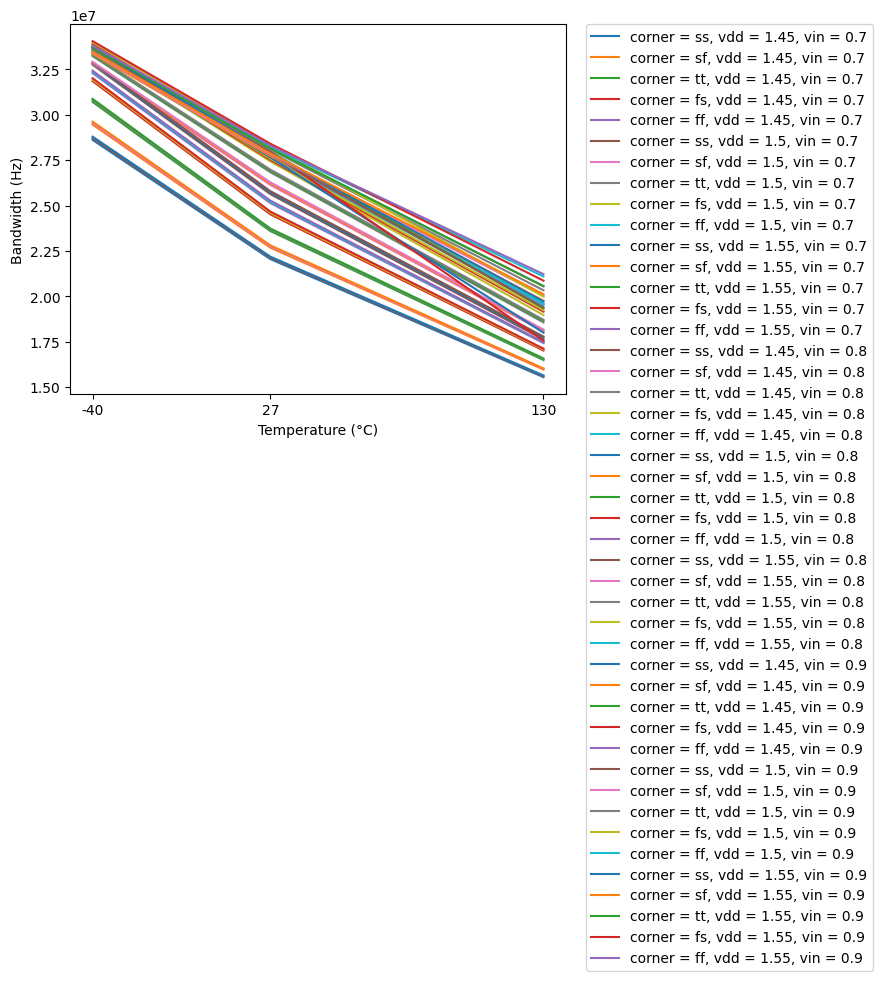
\includegraphics{./cace/_docs/ota-5t/schematic/bw_vs_temp.png}

}

\caption{bw\_vs\_temp}

\end{figure}%

\subsection{bw\_vs\_vin}\label{bw_vs_vin}

\begin{figure}[H]

{\centering 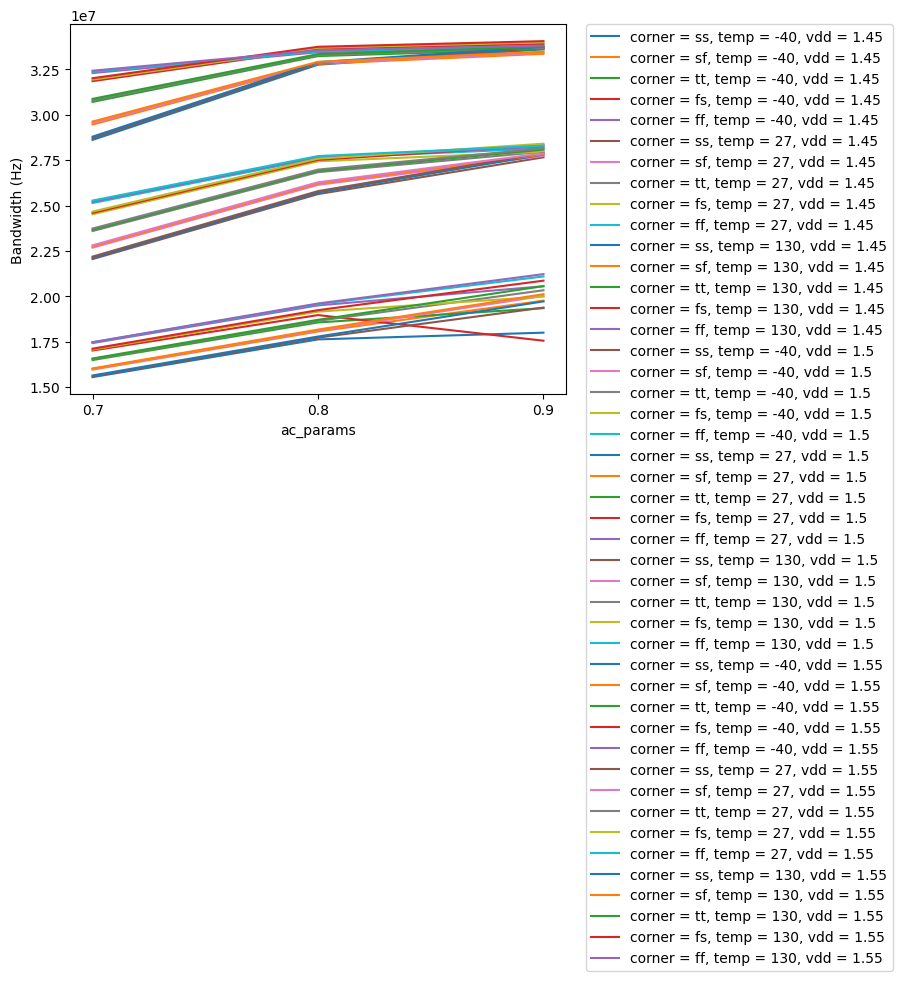
\includegraphics{./cace/_docs/ota-5t/schematic/bw_vs_vin.png}

}

\caption{bw\_vs\_vin}

\end{figure}%

\subsection{bw\_vs\_vdd}\label{bw_vs_vdd}

\begin{figure}[H]

{\centering 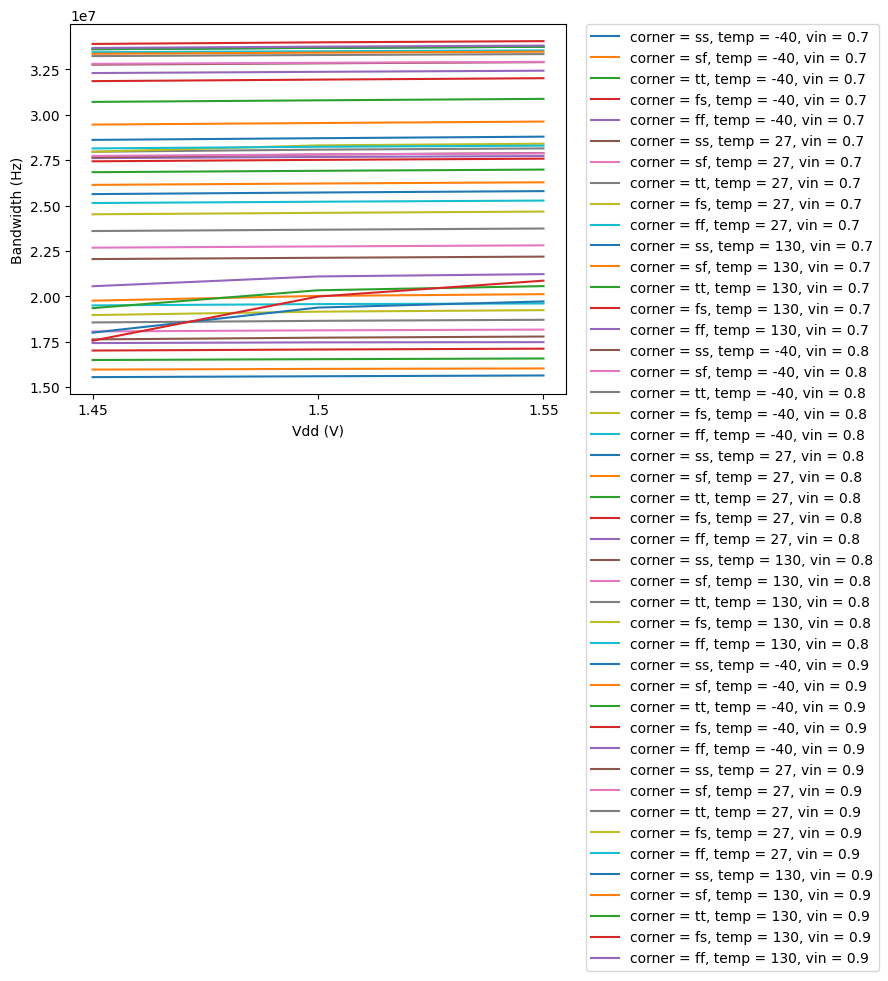
\includegraphics{./cace/_docs/ota-5t/schematic/bw_vs_vdd.png}

}

\caption{bw\_vs\_vdd}

\end{figure}%

\subsection{bw\_vs\_corner}\label{bw_vs_corner}

\begin{figure}[H]

{\centering 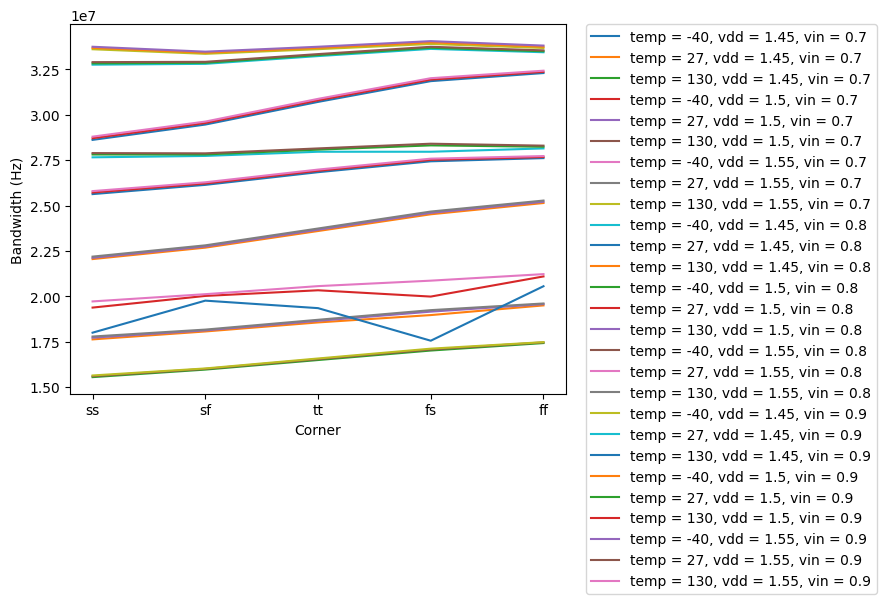
\includegraphics{./cace/_docs/ota-5t/schematic/bw_vs_corner.png}

}

\caption{bw\_vs\_corner}

\end{figure}%

\subsection{noise\_vs\_temp}\label{noise_vs_temp}

\begin{figure}[H]

{\centering 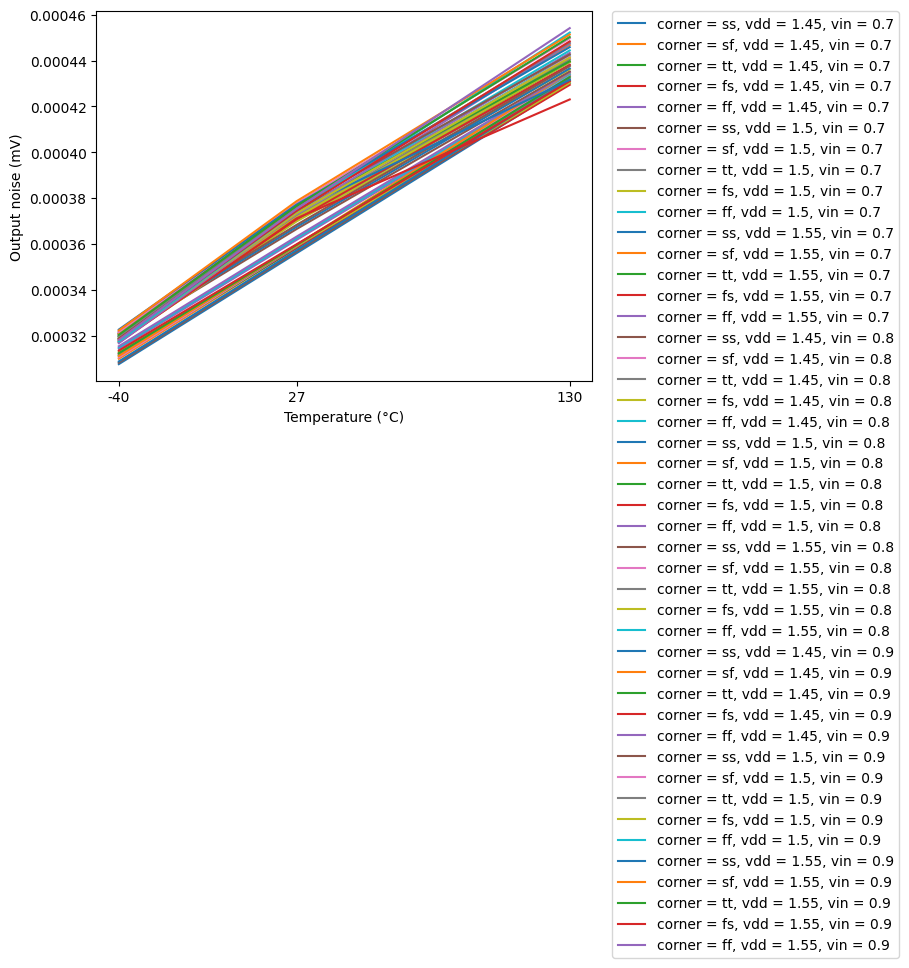
\includegraphics{./cace/_docs/ota-5t/schematic/noise_vs_temp.png}

}

\caption{noise\_vs\_temp}

\end{figure}%

\subsection{noise\_vs\_vin}\label{noise_vs_vin}

\begin{figure}[H]

{\centering 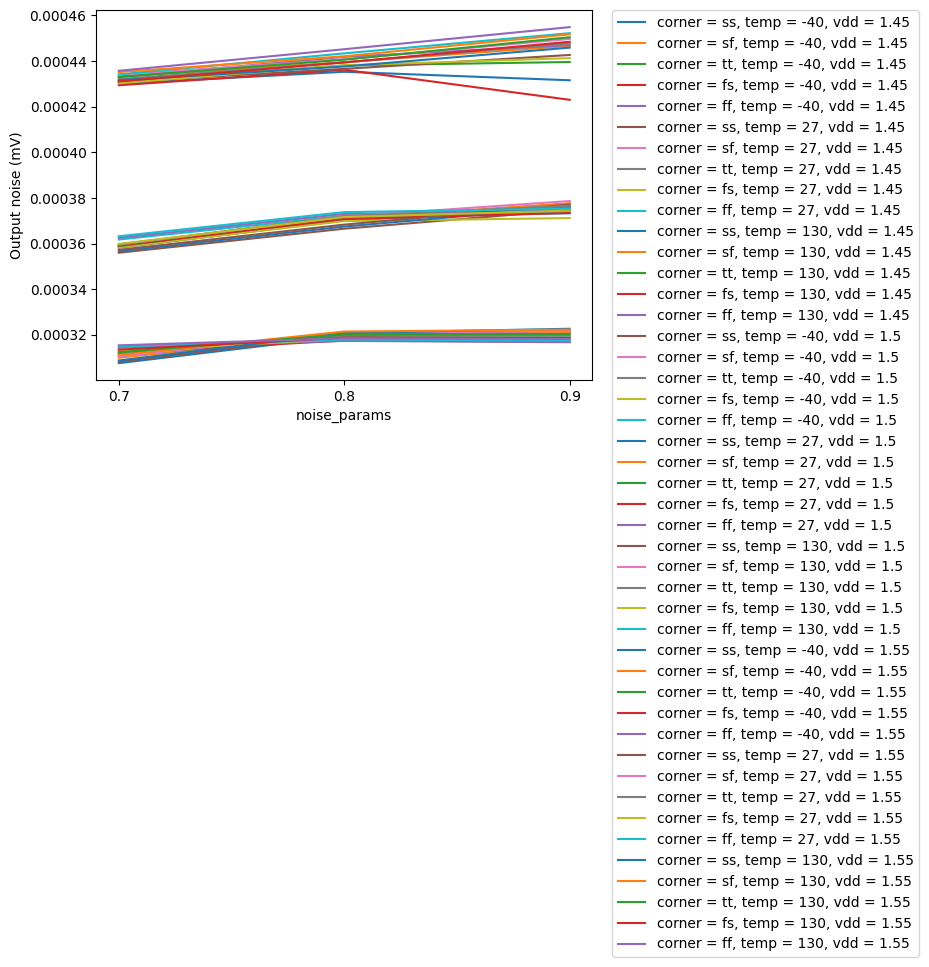
\includegraphics{./cace/_docs/ota-5t/schematic/noise_vs_vin.png}

}

\caption{noise\_vs\_vin}

\end{figure}%

\subsection{noise\_vs\_vdd}\label{noise_vs_vdd}

\begin{figure}[H]

{\centering 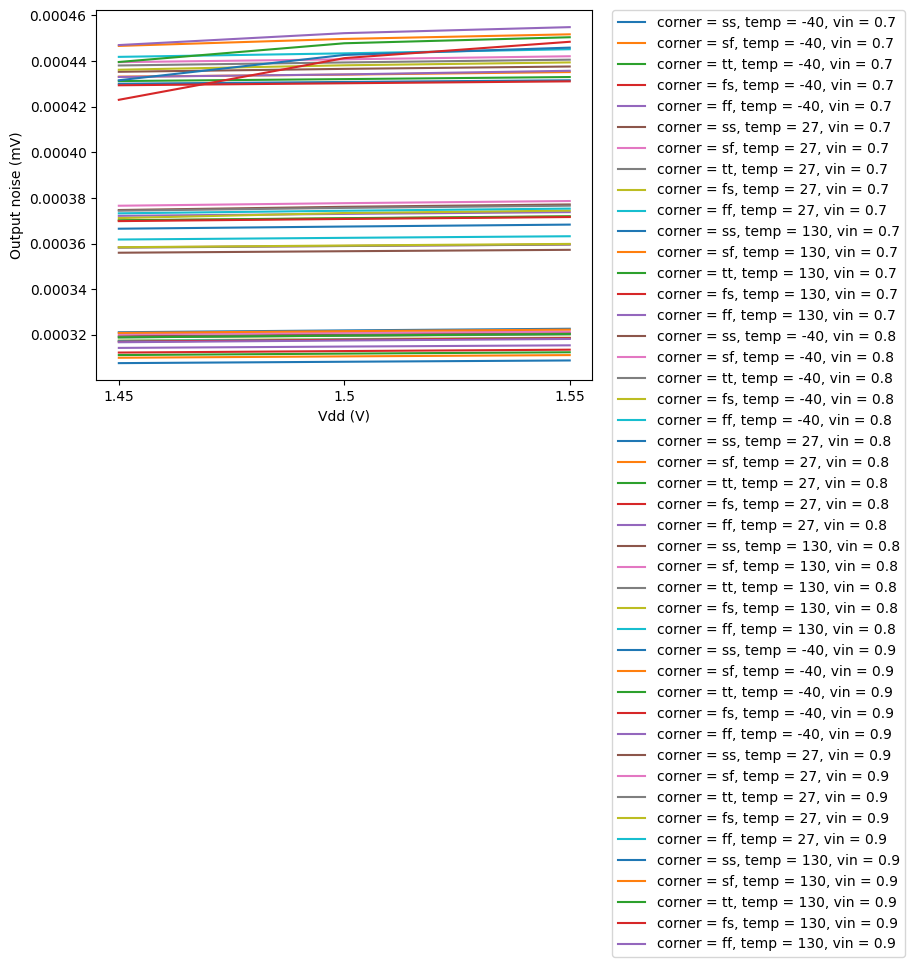
\includegraphics{./cace/_docs/ota-5t/schematic/noise_vs_vdd.png}

}

\caption{noise\_vs\_vdd}

\end{figure}%

\subsection{noise\_vs\_corner}\label{noise_vs_corner}

\begin{figure}[H]

{\centering 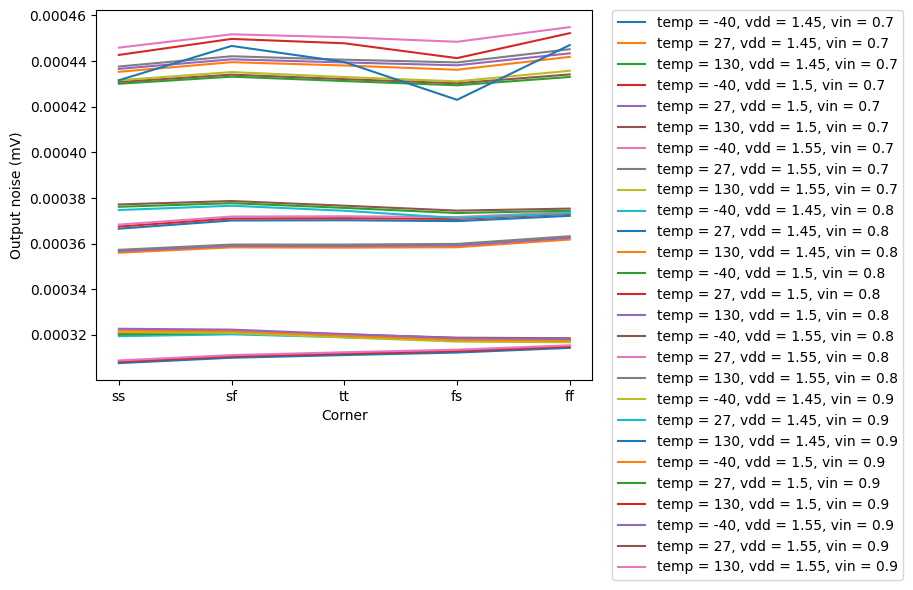
\includegraphics{./cace/_docs/ota-5t/schematic/noise_vs_corner.png}

}

\caption{noise\_vs\_corner}

\end{figure}%

\subsection{settling\_vs\_temp}\label{settling_vs_temp}

\begin{figure}[H]

{\centering 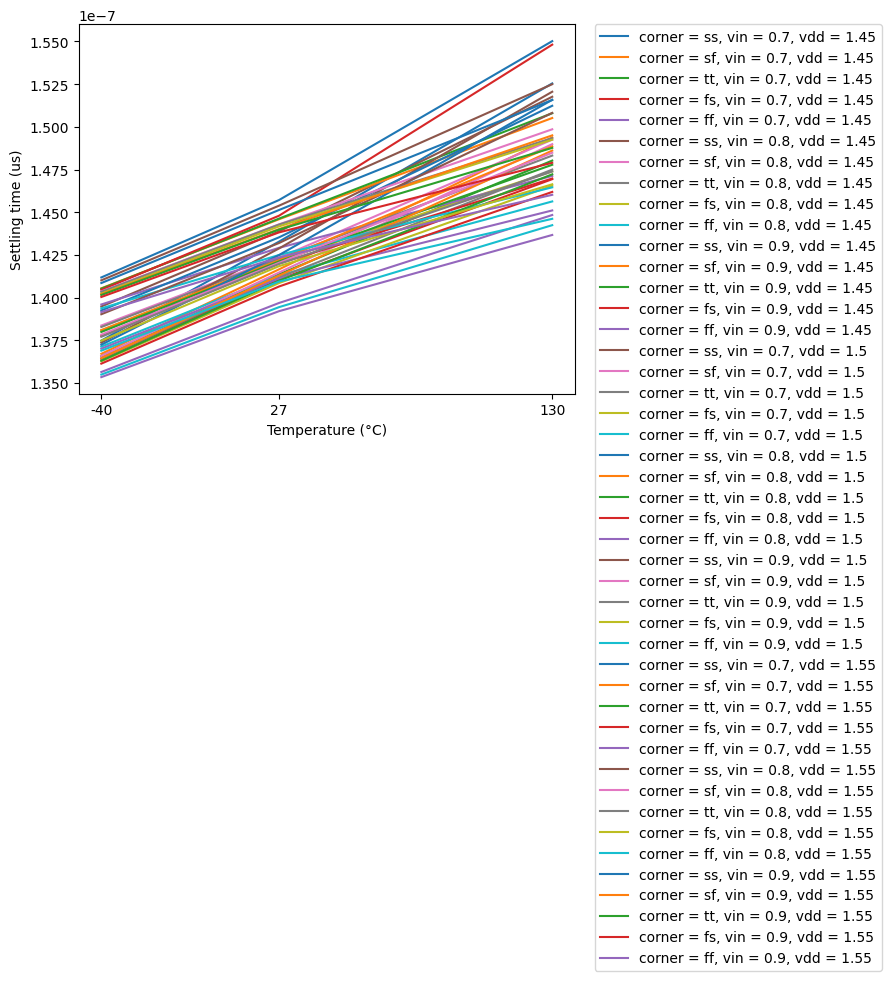
\includegraphics{./cace/_docs/ota-5t/schematic/settling_vs_temp.png}

}

\caption{settling\_vs\_temp}

\end{figure}%

\subsection{settling\_vs\_vin}\label{settling_vs_vin}

\begin{figure}[H]

{\centering \includegraphics{./cace/_docs/ota-5t/schematic/settling_vs_vin.png}

}

\caption{settling\_vs\_vin}

\end{figure}%

\subsection{settling\_vs\_vdd}\label{settling_vs_vdd}

\begin{figure}[H]

{\centering \includegraphics{./cace/_docs/ota-5t/schematic/settling_vs_vdd.png}

}

\caption{settling\_vs\_vdd}

\end{figure}%

\subsection{settling\_vs\_corner}\label{settling_vs_corner}

\begin{figure}[H]

{\centering \includegraphics{./cace/_docs/ota-5t/schematic/settling_vs_corner.png}

}

\caption{settling\_vs\_corner}

\end{figure}%

\end{tcolorbox}

\subsubsection{PVT Simulation Analysis}\label{pvt-simulation-analysis}

Looking at the CACE report in Note~\ref{nte-basic-ota-cace-result} we
see that (luckily) the specifiction is met for all parameters. This is
great news! We now have a design that we carefully simulated across PVT
and other corners, and which is ready for layout. Once we have the
layout ready, we can extract the wiring parasitics (\(R\) and \(C\)) as
well as other layout-dependent effects like
\href{https://global.oup.com/us/companion.websites/9780195170153/pdf/proximityeffectmodels.pdf}{well
proximity}. Using this augmented netlist we can then again use CACE to
check performance across conditions and parameter variations, and if we
still pass all specification points then our design is finished.

\section{Cascode Stage}\label{cascode-stage}

\section{A Fully-Differential OTA}\label{a-fully-differential-ota}

\section{Biasing the OTA}\label{biasing-the-ota}

\section{An RC-OPAMP Filter}\label{an-rc-opamp-filter}

\section{Summary \& Conclusion}\label{summary-conclusion}

\section{Appendix: Middlebrook's Method}\label{sec-middlebrook-method}

When we want to do a closed-loop gain analysis (for stability or other
investigations), we have the need to break the loop at one point, apply
a stimulus, and monitor the response on the other end. By doing this we
want to keep the loading on both ends similar to the original case. To
achieve this, we break the loop at one point by inserting (1) an ac
voltage source, and (2) attach an ac current source, as shown in
Figure~\ref{fig-middlebrook-voltage} and
Figure~\ref{fig-middlebrook-current}. The derivation of this approach is
presented in (Middlebrook 1975), and has the big advantage that loading
is not changed, and the bias points are also correct.

\textsubscript{Source:
\href{https://iic-jku.github.io/analog-circuit-design/index.qmd.html}{Article
Notebook}}

\begin{figure}[H]

\centering{

\includegraphics{index_files/mediabag/index_files/figure-pdf/fig-middlebrook-voltage-output-1.pdf}

}

\caption{\label{fig-middlebrook-voltage}Middlebrook voltage loop gain
simulation.}

\end{figure}%

\textsubscript{Source:
\href{https://iic-jku.github.io/analog-circuit-design/index.qmd.html}{Article
Notebook}}

\begin{figure}[H]

\centering{

\includegraphics{index_files/mediabag/index_files/figure-pdf/fig-middlebrook-current-output-1.pdf}

}

\caption{\label{fig-middlebrook-current}Middlebrook current loop gain
simulation.}

\end{figure}%

\textsubscript{Source:
\href{https://iic-jku.github.io/analog-circuit-design/index.qmd.html}{Article
Notebook}}

For both cases we do an ac analysis, and find the corresponding transfer
functions \(T_\mathrm{v}\) and \(T_\mathrm{i}\) as \[
T_\mathrm{v} = -\frac{V_\mathrm{r}}{V_\mathrm{f}}
\] and \[
T_\mathrm{i} = -\frac{I_\mathrm{r}}{I_\mathrm{f}}.
\]

Then, we can calculate the closed-loop transfer function
\(T(s) = H_\mathrm{ol(s)}\) as \[
T(s) = \frac{T_\mathrm{v} T_\mathrm{i} - 1}{T_\mathrm{v} + T_\mathrm{i} + 2}.
\]

\section{Appendix: ngspice
Cheatsheet}\label{appendix-ngspice-cheatsheet}

Here is an unsorted list of useful ngspice settings and command:

\subsubsection{Commands}\label{commands}

\begin{itemize}
\tightlist
\item
  \texttt{ac\ dec\textbar{}lin\ points\ fstart\ fstop} performs a
  small-signal ac analysis with either linear or decade sweep
\item
  \texttt{dc\ sourcename\ vstart\ vstop\ vincr\ {[}src2\ start2\ stop2\ incr2{]}}
  runs a dc-sweep, optionally across two variables
\item
  \texttt{display} shows the available data vectors in the current plot
\item
  \texttt{echo} can be used to display text, \texttt{\$variable} or
  \texttt{\$\&vector}, can be useful for debugging
\item
  \texttt{let\ name\ =\ expr} to create a new vector;
  \texttt{unlet\ vector} deletes a specified vector; access vector data
  with \texttt{\$\&vec}
\item
  \texttt{linearize\ vec} linearizes a vector on an equidistant time
  scale, do this before an FFT; with \texttt{set\ specwindow=windowtype}
  a proper windowing function can be set
\item
  \texttt{meas} can be used for various evaluations of measurement
  results (see ngspice manual for details)
\item
  \texttt{noise\ v(output\ \textless{}ref\textgreater{})\ src\ (dec\textbar{}lin)\ pts\ fstart\ fstop}
  runs a small-signal noise analysis
\item
  \texttt{op} calculates the operating point, useful for checking bias
  points and device parameters
\item
  \texttt{plot\ expr\ vs\ scale} to plot something
\item
  \texttt{print\ expr} to print it, use \texttt{print\ all} to print
  everything
\item
  \texttt{remzerovec} can be useful to remove vectors with zero length,
  which otherwise cause issues when saving or plotting data
\item
  \texttt{rusage} plot information about resource usage like memory
\item
  \texttt{save\ all} or \texttt{save\ signal} specifies which data is
  saved during simulation; this lowers RAM usage during simulation and
  size of RAW file; do save before the actual simulation statement
\item
  \texttt{setplot} show a list of available plots
\item
  \texttt{set\ var\ =\ value} to set the value of a variable; use
  variable with \texttt{\$var}; \texttt{unset\ var} removes a variable
\item
  \texttt{set\ enable\_noisy\_r} to enable noise of behavioral
  resistors; usually, this is a good idea
\item
  \texttt{shell\ cmd} to run a shell command
\item
  \texttt{show\ :\ param}, like \texttt{show\ :\ gm} shows the
  \(g_\mathrm{m}\) of all devices after running an operating point with
  \texttt{op}
\item
  \texttt{spec} plots a spectrum (i.e.~frequency domain plot)
\item
  \texttt{status} shows the saved parameters and nodes
\item
  \texttt{tf} runs a transfer function analysis, returning transfer
  function, input and output resistance
\item
  \texttt{tran\ tstep\ tstop\ \textless{}tstart\ \textless{}tmax\textgreater{}\textgreater{}}
  runs a transient analysis until \texttt{tstop}, reporting results with
  \texttt{tstep} stepsize, starting to plot at \texttt{tstart} and
  performs time steps not larger then \texttt{tmax}
\item
  \texttt{wrdata} writes data into a file in a tabular ASCII format;
  easy to further process
\item
  \texttt{write} writes simulation data (the saved nodes) into a RAW
  file; default is binary, can be changed to ASCII with
  \texttt{set\ filetype=ascii}; with \texttt{set\ appendwrite} data is
  added to an existing file
\end{itemize}

\subsubsection{Options}\label{options}

Use \texttt{option\ option=val\ option=val} to set various options;
important ones are:

\begin{itemize}
\tightlist
\item
  \texttt{abstol} sets the absolute current error tolerance (default is
  1pA)
\item
  \texttt{gmin} is the conductance applied at every node for convergence
  improvement (default is 1e-12); this can be critical for very high
  impedance circuits
\item
  \texttt{klu} sets the KLU matrix solver
\item
  \texttt{list} print the summary listing of the input data
\item
  \texttt{maxord} sets the numerical order of the integration method
  (default is 2 for Gear)
\item
  \texttt{method} set the numerical integration method to \texttt{gear}
  or \texttt{trap} (default is \texttt{trap})
\item
  \texttt{node} prints the node table
\item
  \texttt{opts} prints the option values
\item
  \texttt{temp} sets the simulation temperature
\item
  \texttt{reltol} set the relative error tolerance (default is 0.001 =
  0.1\%)
\item
  \texttt{savecurrents} saves the terminal currents of all devices
\item
  \texttt{sparse} sets the sparse matrix solver, which can run noise
  analysis, but is slower than \texttt{klu}
\item
  \texttt{vntol} sets the absolute voltage error tolerance (default is
  1µV)
\item
  \texttt{warn} enables the priting of the SOA warning messages
\end{itemize}

\subsubsection{Convergence Helper}\label{convergence-helper}

\begin{itemize}
\tightlist
\item
  \texttt{option\ gmin} can be used to increase the conductance applied
  at every node
\item
  \texttt{option\ method=gear} can lead to improved convergence
\item
  \texttt{.nodeset} can be used to specify initial node voltage guesses
\item
  \texttt{.ic} can be used to set initial conditions
\end{itemize}

\section{Appendix: Xschem Cheatsheet}\label{appendix-xschem-cheatsheet}

When opening Xschem, using \texttt{Help\ -\textgreater{}\ Keys} a pop-up
windows comes up with many useful shortcuts. The most useful are:

\paragraph{Moving around in a
schematic:}\label{moving-around-in-a-schematic}

\begin{itemize}
\tightlist
\item
  \texttt{Cursor\ keys} to move around
\item
  \texttt{Ctrl-e} to go back to parent schematic
\item
  \texttt{e} to descend into selected symbol
\item
  \texttt{f} full zoom on schematic
\item
  \texttt{Shift-z} to zoom in
\item
  \texttt{Ctrl-z} to zoom out
\end{itemize}

\paragraph{Editing schematics:}\label{editing-schematics}

\begin{itemize}
\tightlist
\item
  \texttt{Del} to delete elements
\item
  \texttt{Ins} to insert elements from library
\item
  \texttt{Escape} to abort an operation
\item
  \texttt{Ctrl-\#} to rename components with duplicate names
\item
  \texttt{c} to copy elements
\item
  \texttt{Alt-Shift-l} to add wire lable
\item
  \texttt{Alt-l} to add lable pin
\item
  \texttt{m} move selected objects
\item
  \texttt{q} to edit properties
\item
  \texttt{Ctrl-s} to save schematic
\item
  \texttt{t} to place a text
\item
  \texttt{Shift-T} to toggle the \texttt{ignore} flag on an instance
\item
  \texttt{u} to undo an operation
\item
  \texttt{w} to draw a wire
\item
  \texttt{Shift-W} draw wire and snap to close pin or netpoint
\item
  \texttt{\&} to join, break, and collapse wires
\end{itemize}

\paragraph{Viewing/Simulating
Schematics}\label{viewingsimulating-schematics}

\begin{itemize}
\tightlist
\item
  \texttt{5} to only view probes
\item
  \texttt{k} to highlight selected net
\item
  \texttt{Shift-K} to unhighlight all nets
\item
  \texttt{Shift-o} to toggle light/dark color scheme
\item
  \texttt{s} to run a simulation
\end{itemize}

\textsubscript{Source:
\href{https://iic-jku.github.io/analog-circuit-design/index.qmd.html}{Article
Notebook}}

\phantomsection\label{refs}
\begin{CSLReferences}{1}{0}
\bibitem[\citeproctext]{ref-Hellen_2003}
Hellen, Edward H. 2003. {``{Verifying the diode--capacitor circuit
voltage decay}.''} \emph{American Journal of Physics} 71 (8): 797--800.
\url{https://doi.org/10.1119/1.1578070}.

\bibitem[\citeproctext]{ref-Chenming_Hu_2010}
Hu, Chenming. 2010. \emph{Modern Semiconductor Devices for Integrated
Circuits}. Pearson.

\bibitem[\citeproctext]{ref-Jespers_Murmann_2017}
Jespers, Paul G. A., and Boris Murmann. 2017. \emph{Systematic Design of
Analog CMOS Circuits: Using Pre-Computed Lookup Tables}. Cambridge
University Press.

\bibitem[\citeproctext]{ref-Middlebrook_1975}
Middlebrook, R. D. 1975. {``{Measurement of loop gain in feedback
systems}.''} \emph{International Journal of Electronics} 38 (4):
485--512. \url{https://doi.org/10.1080/00207217508920421}.

\bibitem[\citeproctext]{ref-Nagel_1975}
Nagel, Laurence W. 1975. {``SPICE2: A Computer Program to Simulate
Semiconductor Circuits.''} PhD thesis, EECS Department, University of
California, Berkeley.
\url{http://www2.eecs.berkeley.edu/Pubs/TechRpts/1975/9602.html}.

\bibitem[\citeproctext]{ref-Tsividis_McAndrew_2011}
Tsividis, Yannis, and Colin McAndrew. 2011. \emph{Operation and Modeling
of the MOS Transistor}. Oxford University Press.

\end{CSLReferences}




\end{document}
